\documentclass[UTF8]{ctexart}

\usepackage{geometry}% 版面大小
\geometry{a4paper,scale=0.7}

\usepackage{graphicx}
\usepackage{caption2}
\usepackage{subfigure}
\usepackage{float}

\usepackage[hidelinks]{hyperref}

\title{作业1}
\author{刘时宜 201180078}
\date{\today}

\begin{document}
    \maketitle
    \tableofcontents
    \section{安装VMware}
    由于之前已经安装过VMware 16 pro版本,且已经配置完成了一些虚拟机,破坏环境重新安装可能会带来意想不到的后果。与刘知豪助教沟通后,其同意跳过这一步骤,不重新安装。系统软件安装信息如下:
    \begin{figure}[H]
        \centering
        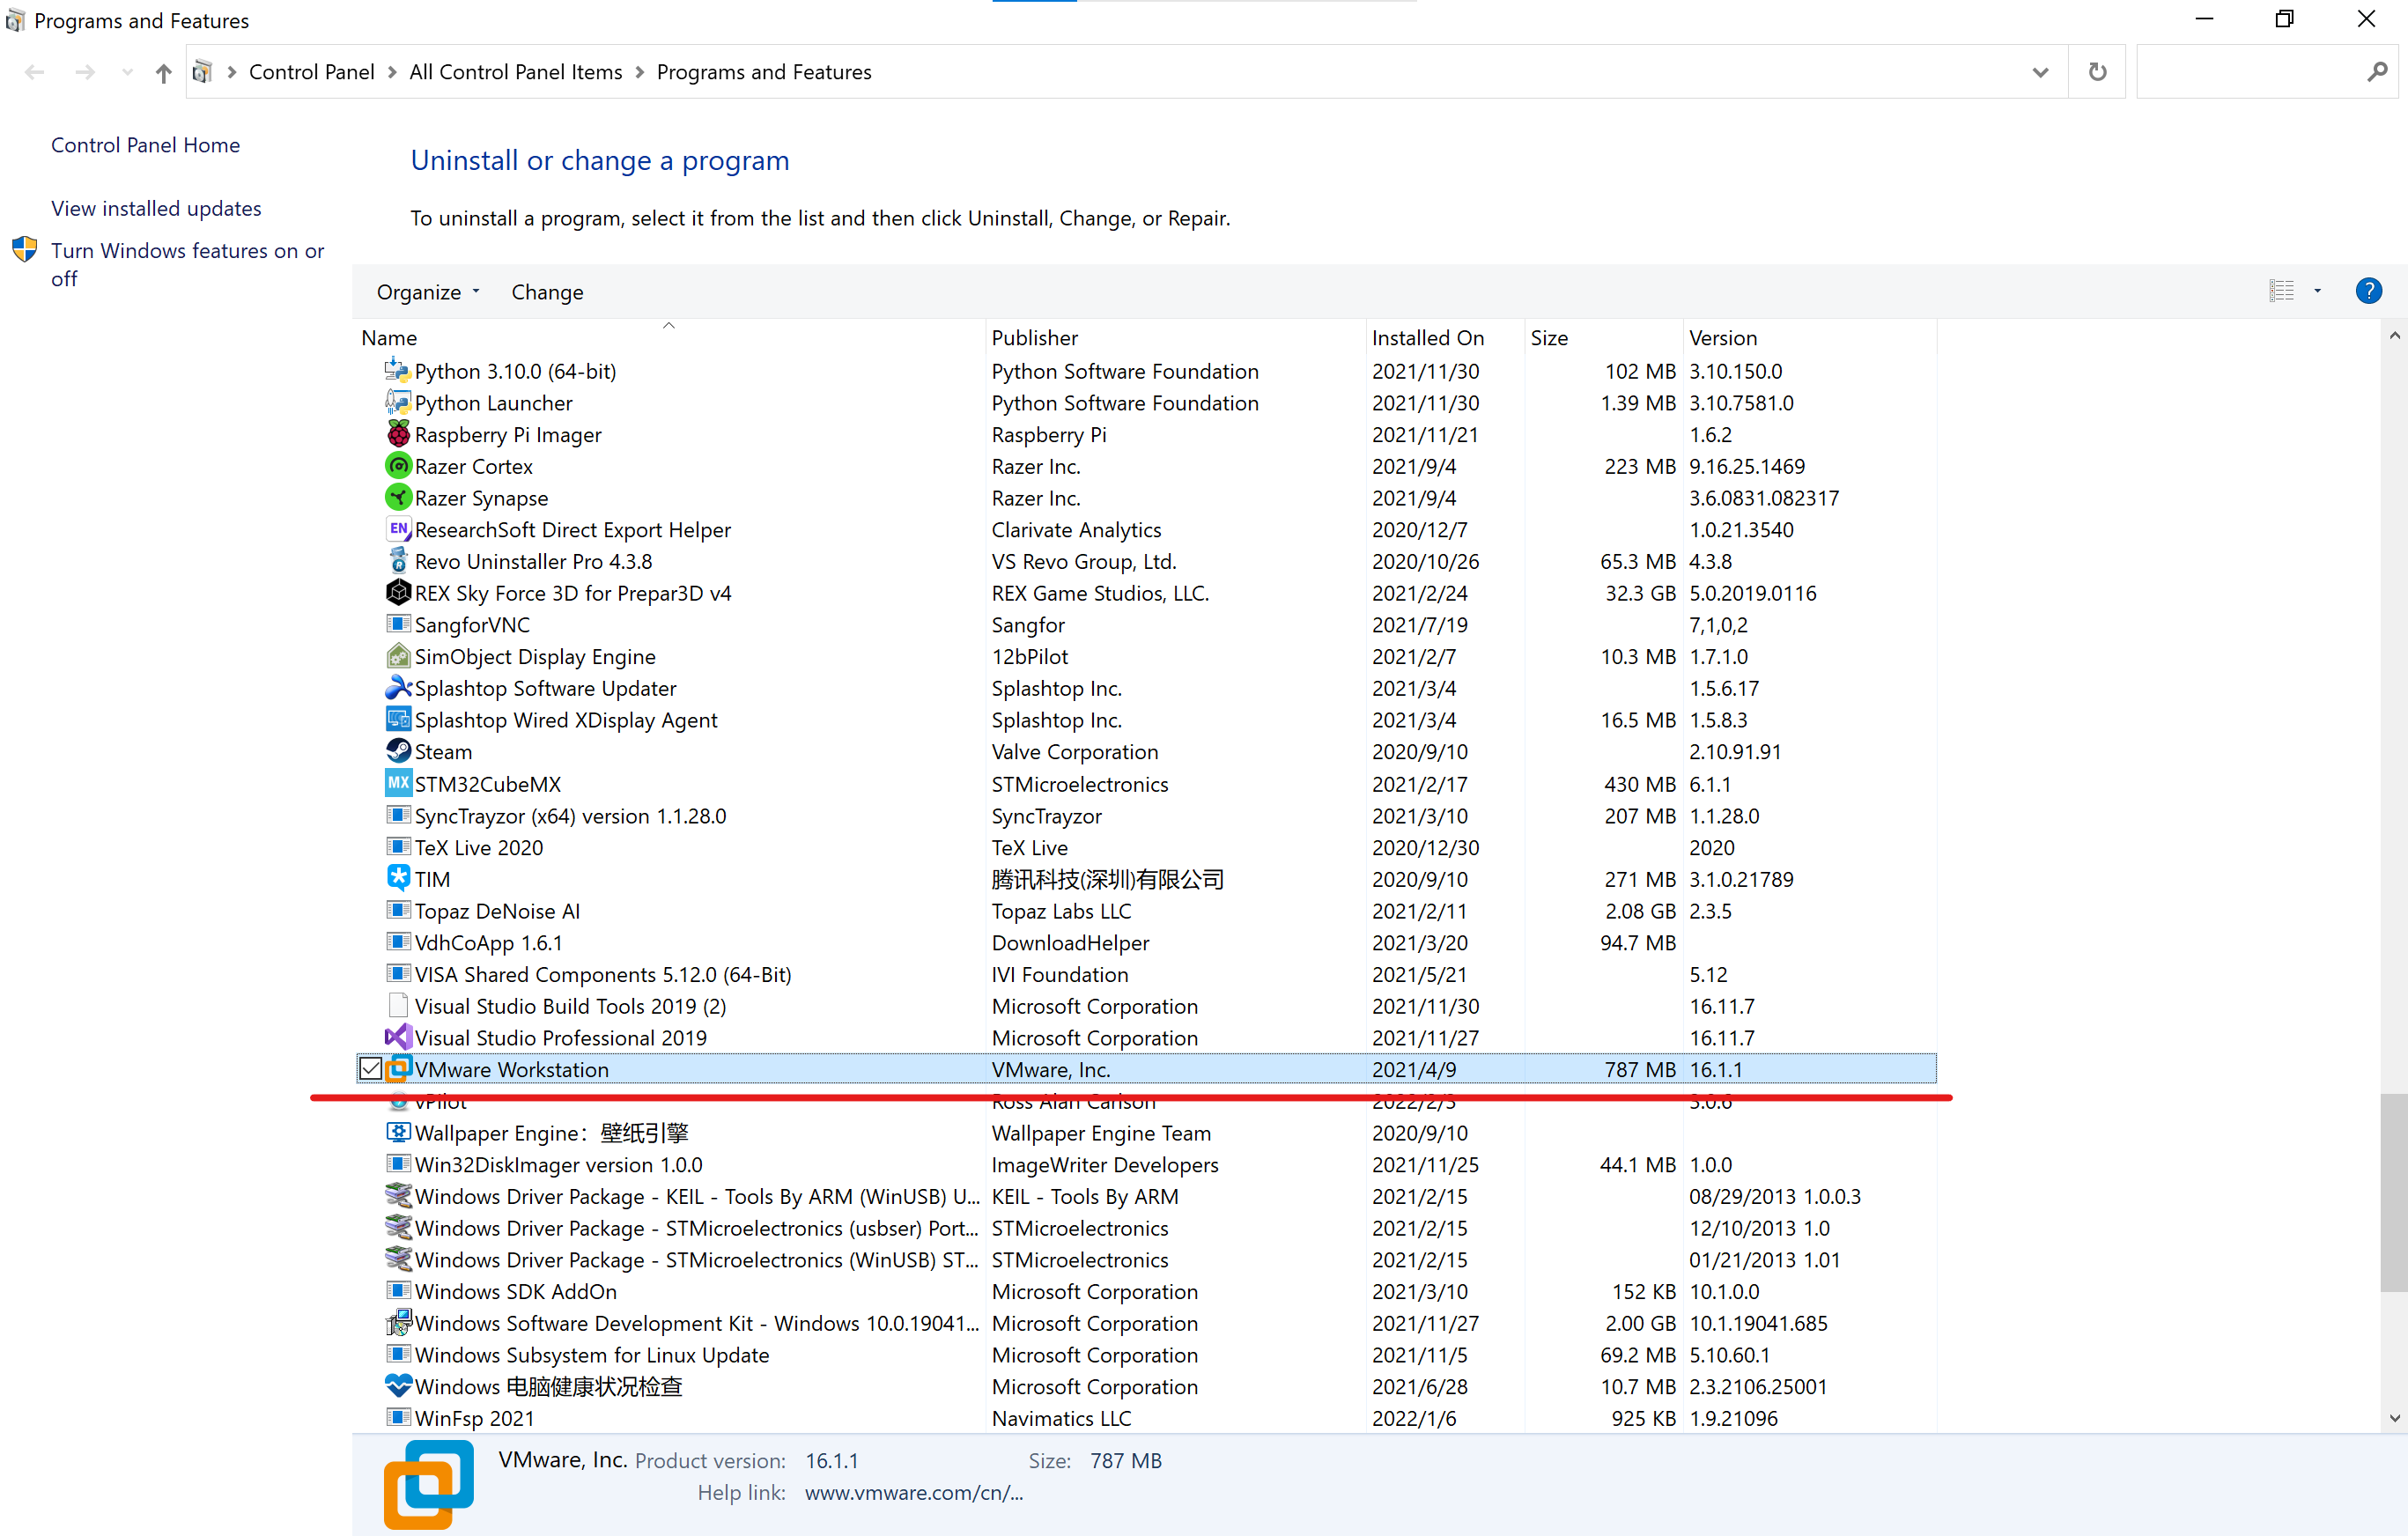
\includegraphics[width=0.8\textwidth]{assets/vmware_install.png}
        \caption{VMware 安装信息}
    \end{figure}

    \section{安装Ubuntu 20.04.3 LTS}
    下载Ubuntu包:
    \begin{figure}[H]
        \centering
        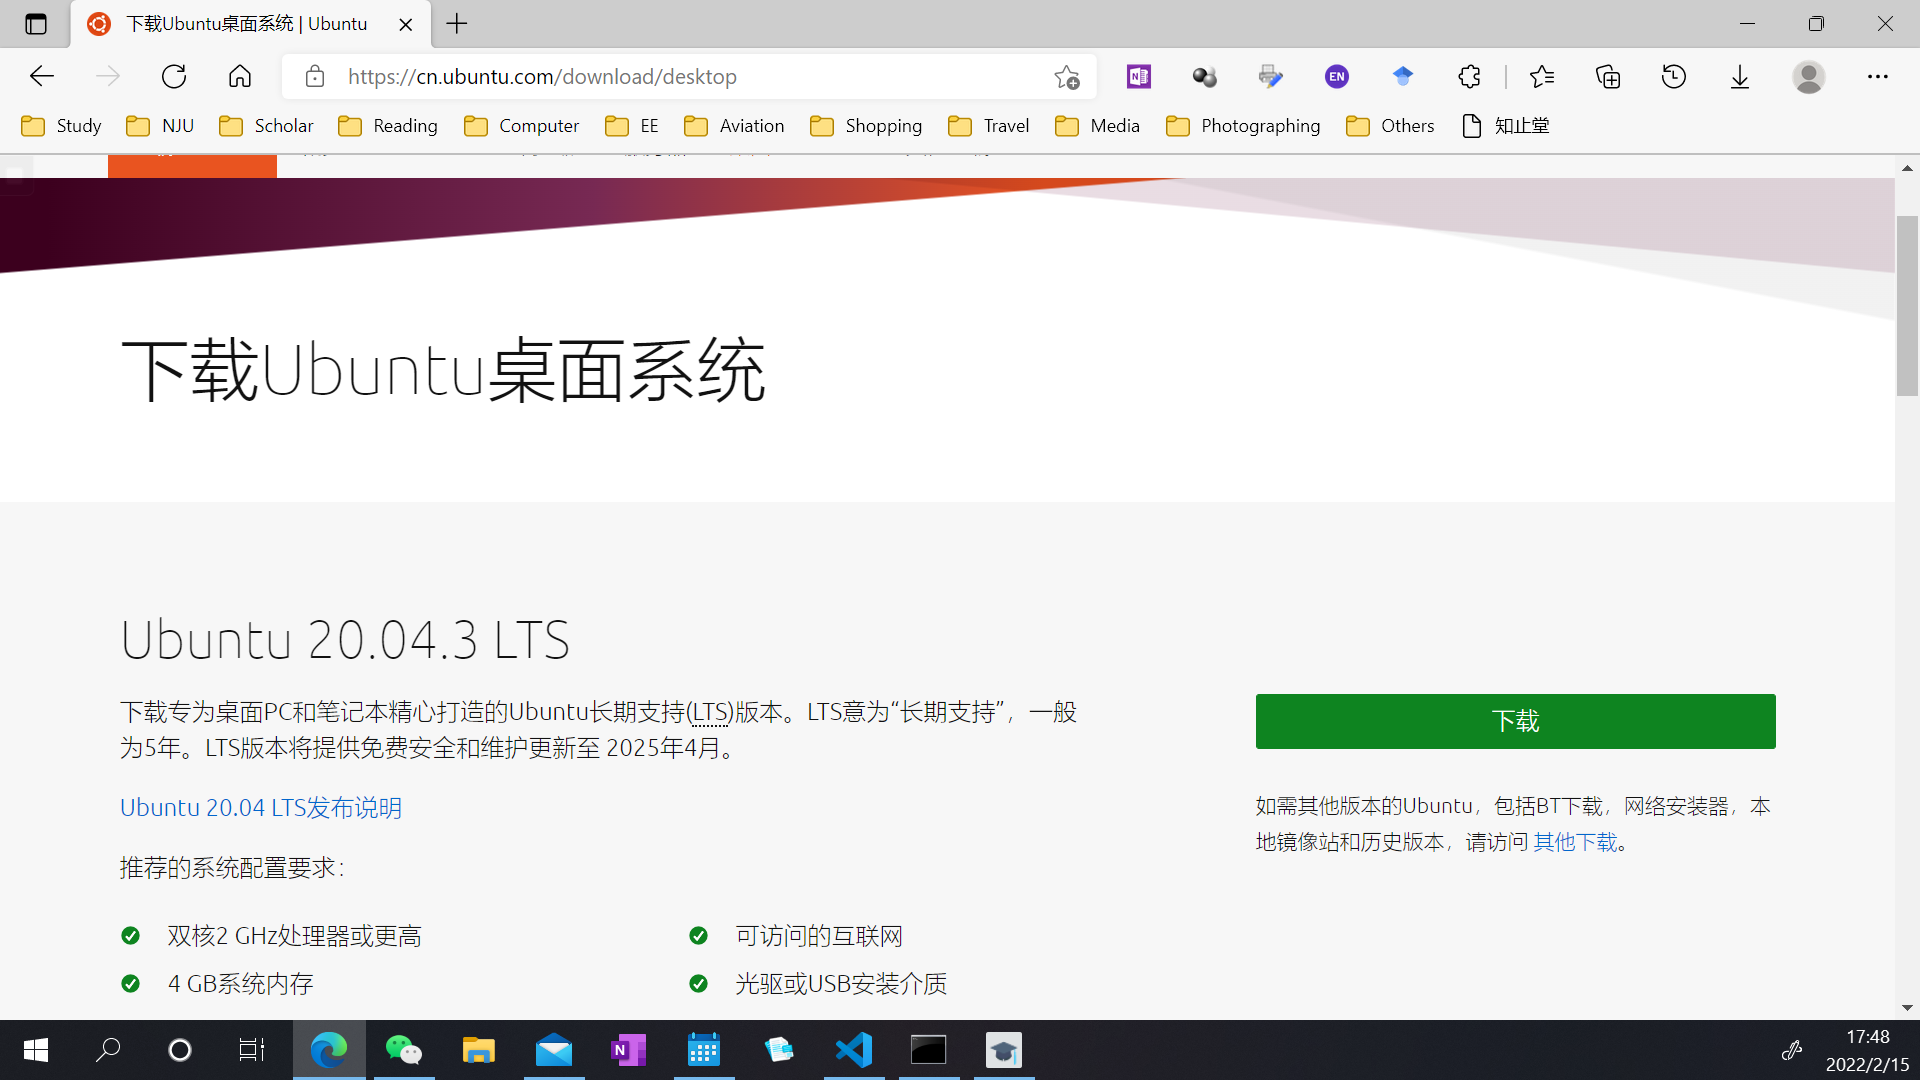
\includegraphics[width=0.8\textwidth]{assets/u1.png}
    \end{figure}

    在VMware中创建虚拟机:
    \begin{figure}[H]
        \centering
        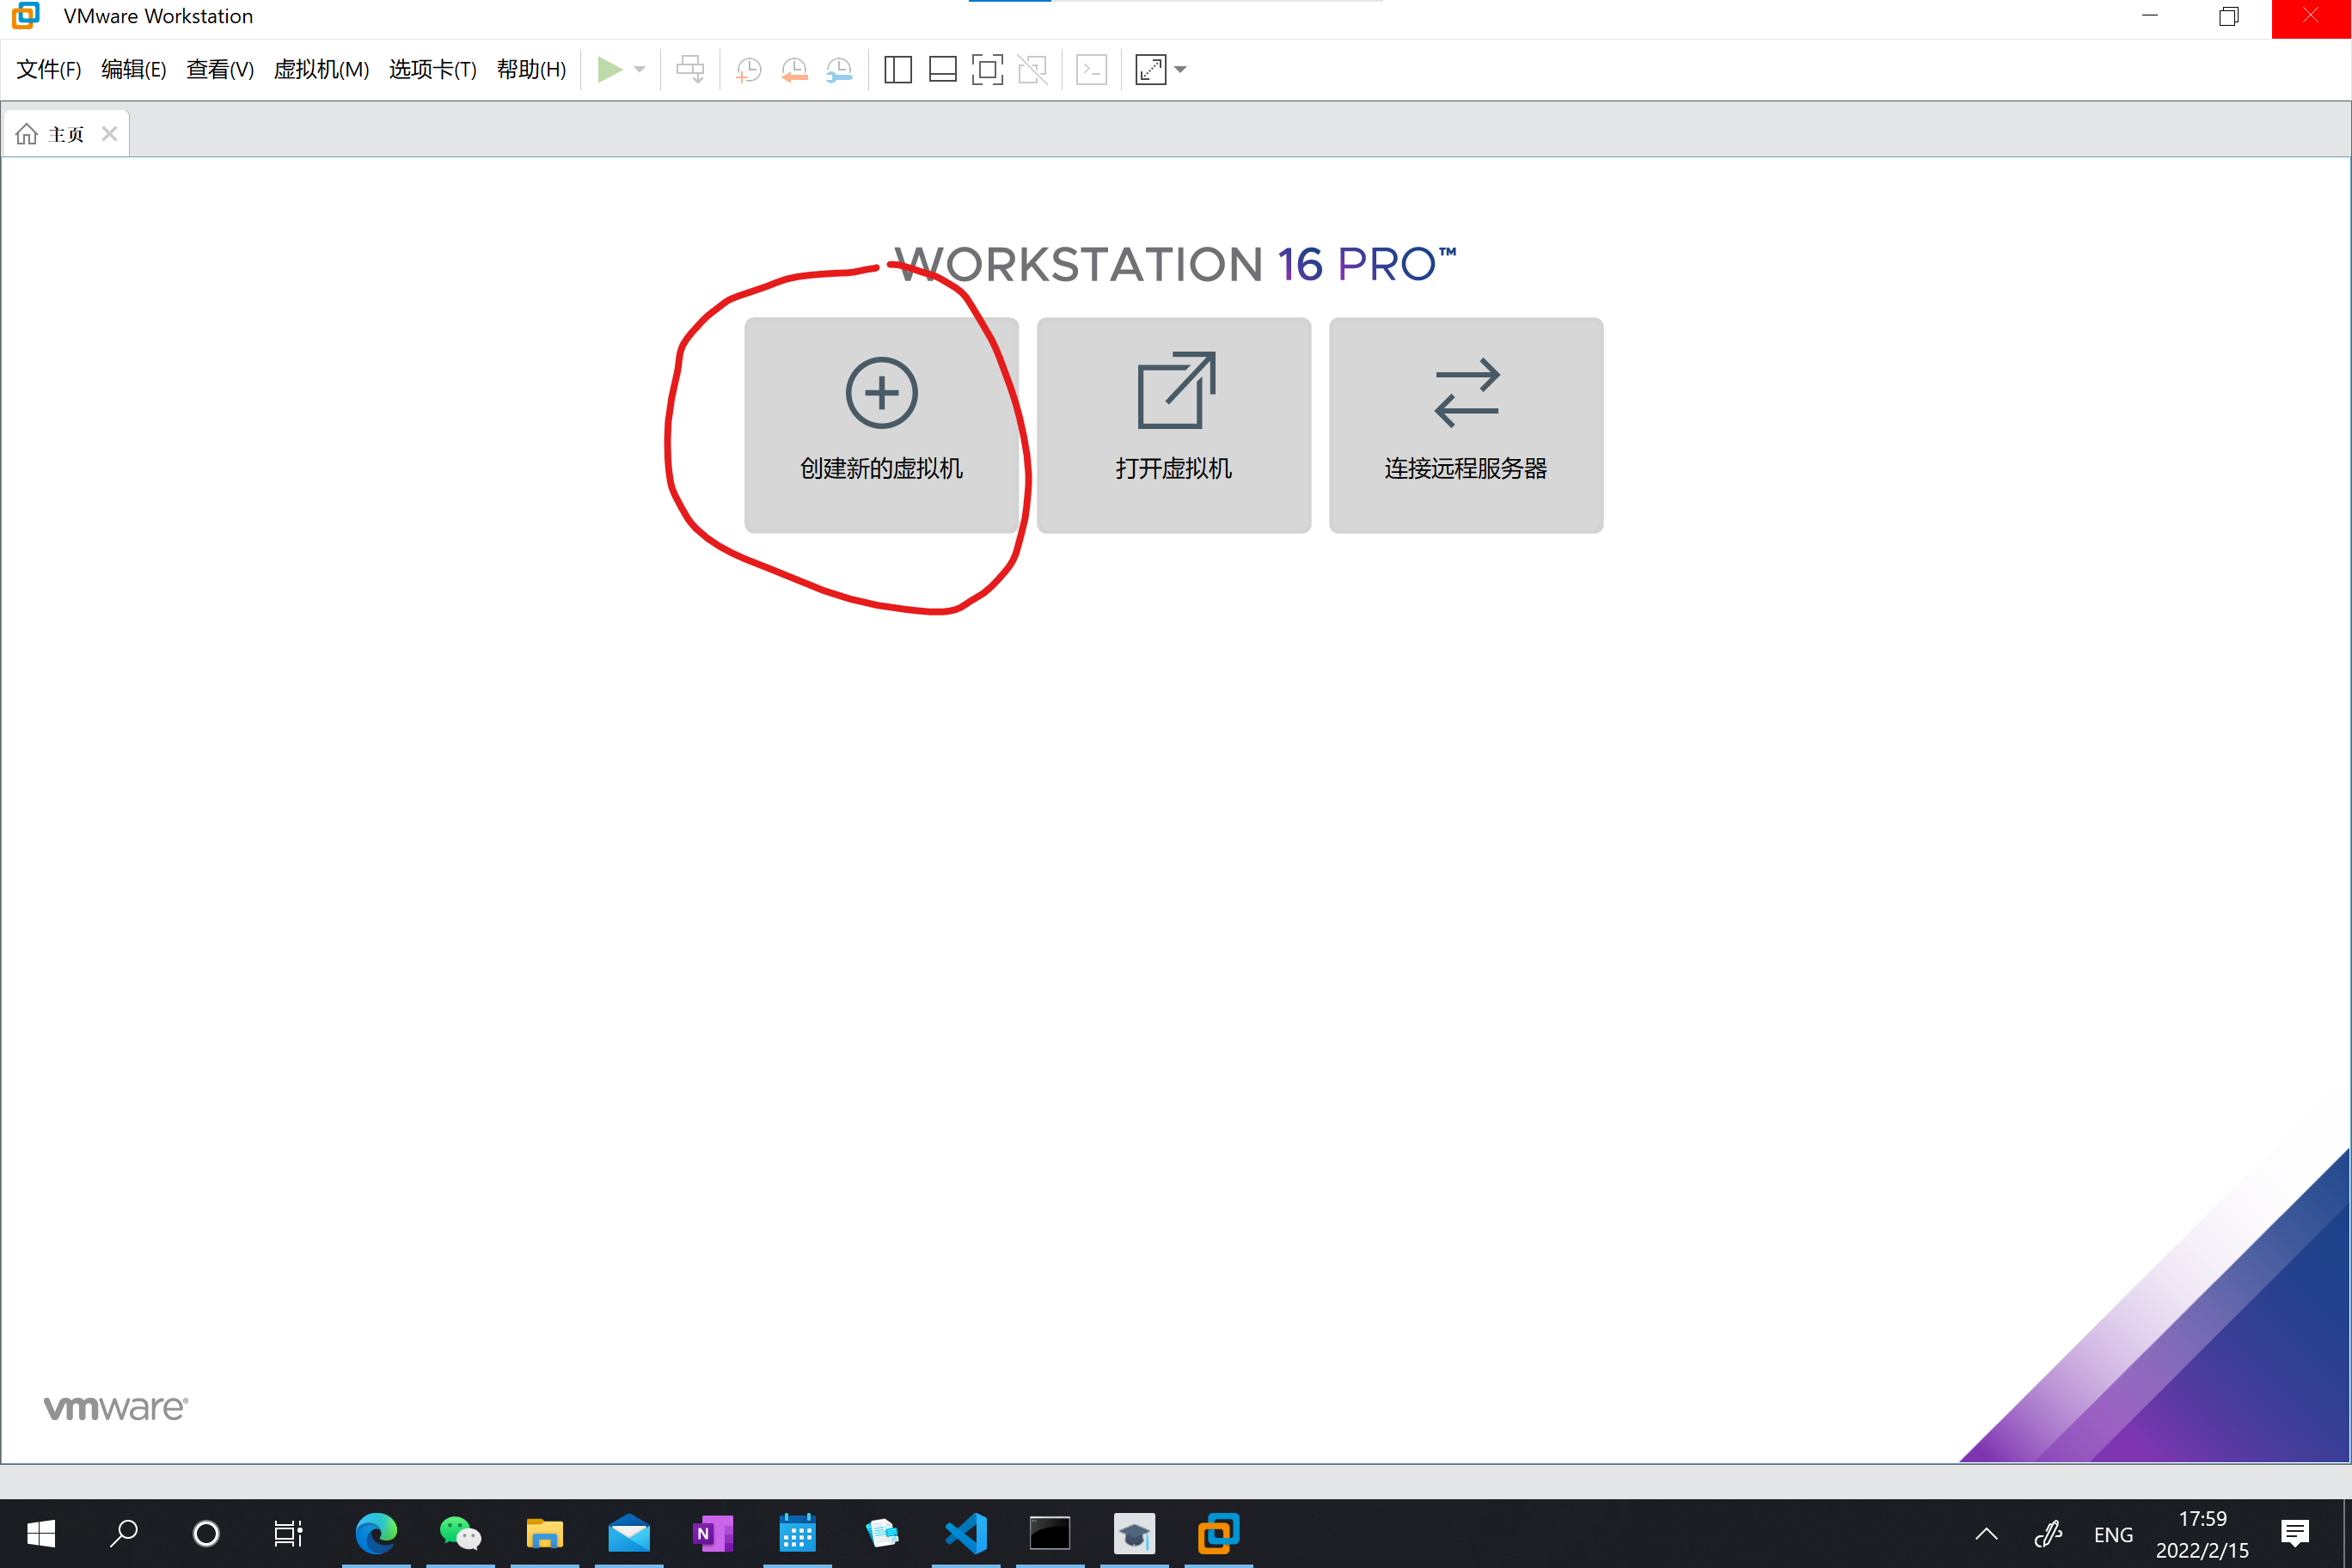
\includegraphics[width=0.8\textwidth]{assets/u2.png}
    \end{figure}
    \begin{figure}[H]
        \centering
        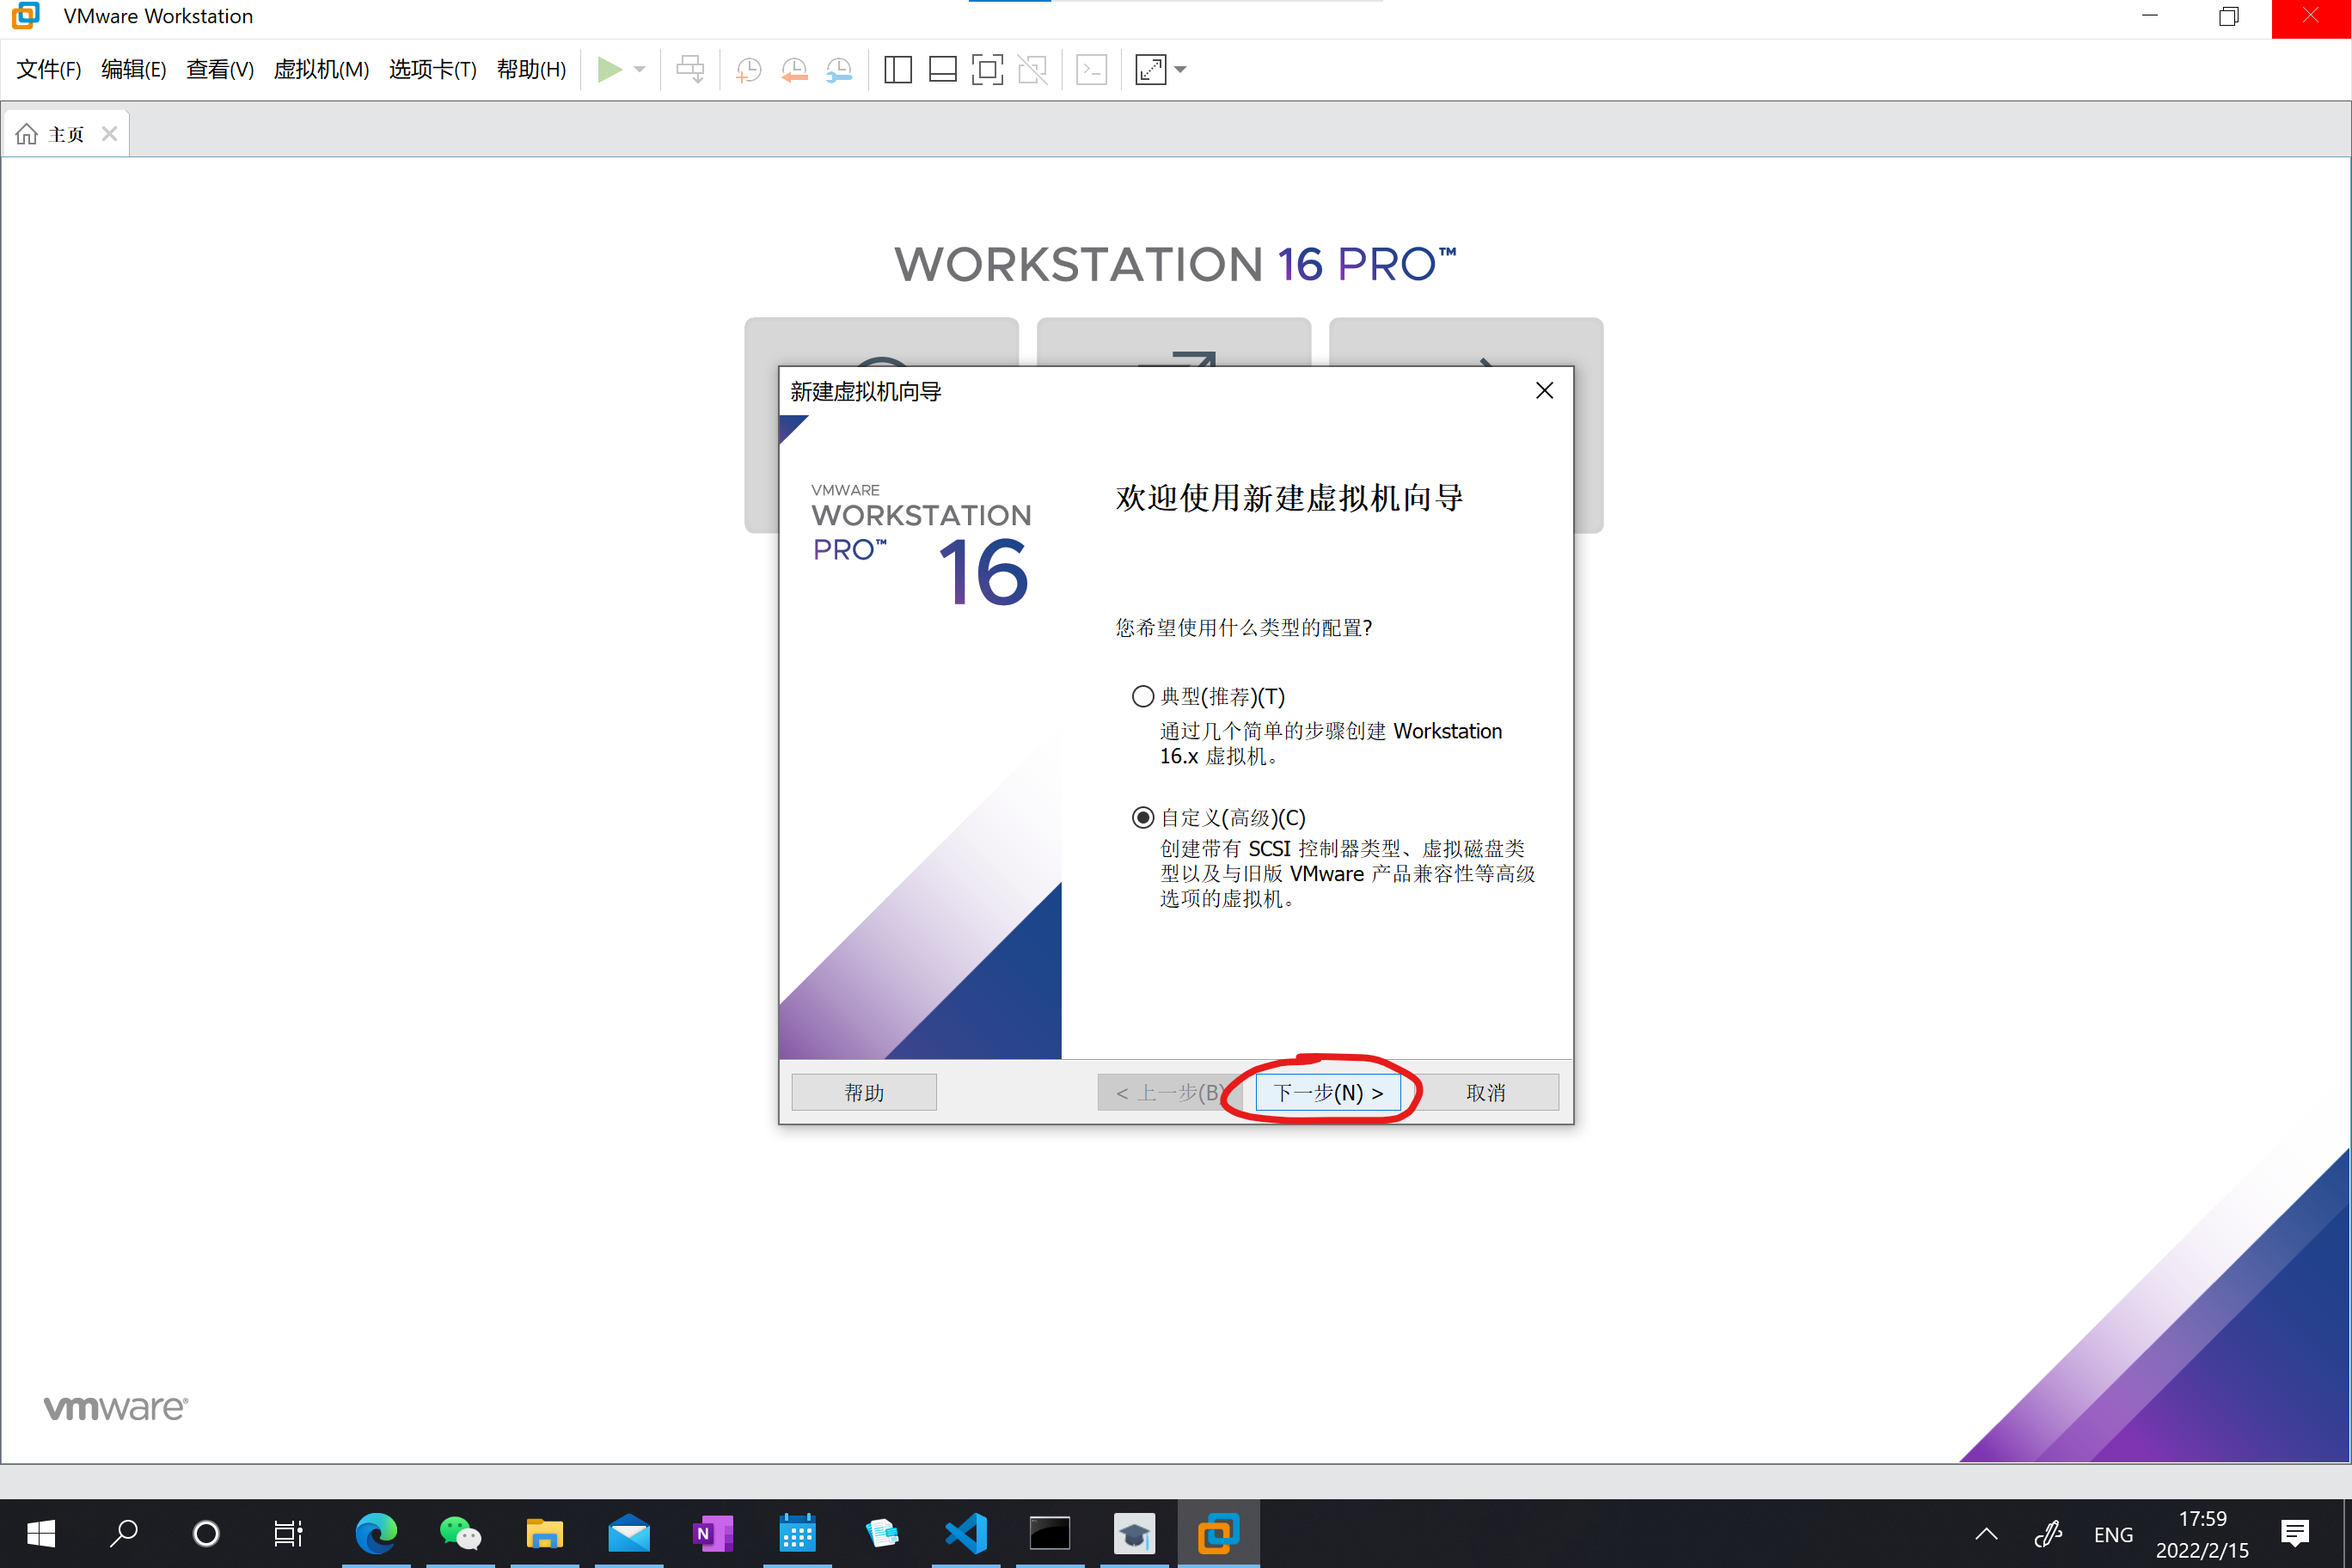
\includegraphics[width=0.8\textwidth]{assets/u3.png}
    \end{figure}
    \begin{figure}[H]
        \centering
        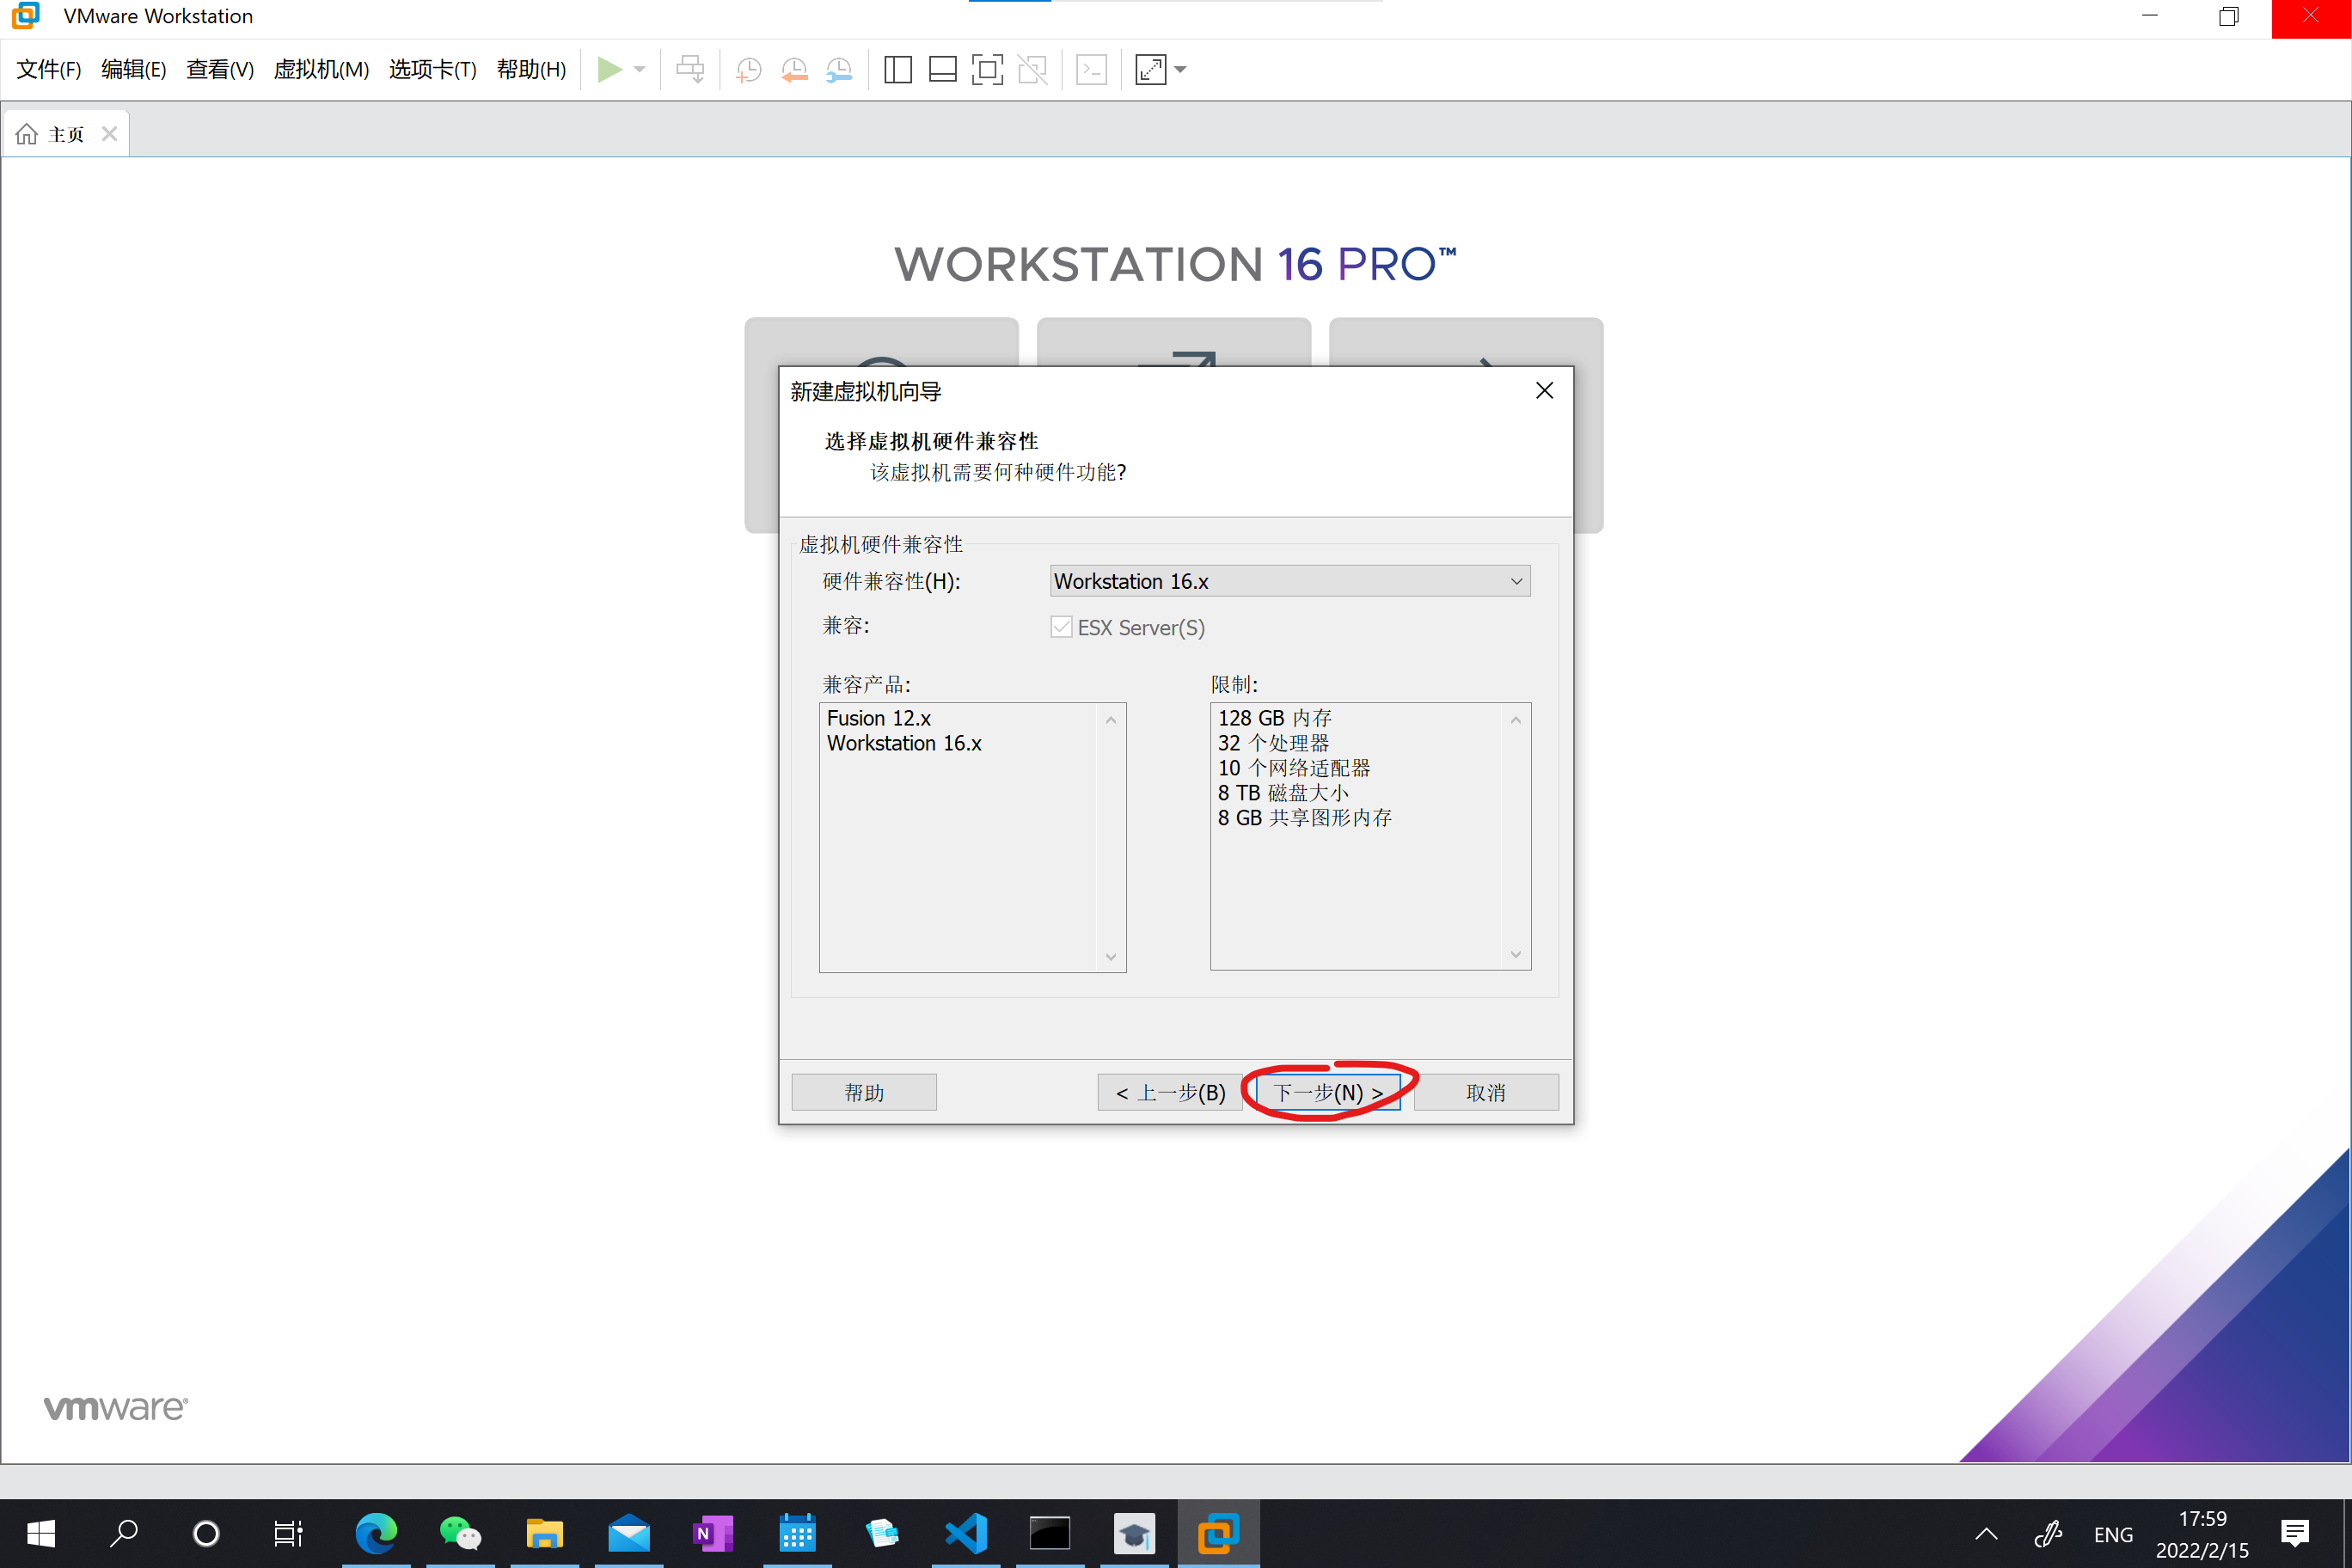
\includegraphics[width=0.8\textwidth]{assets/u4.png}
    \end{figure}
    \begin{figure}[H]
        \centering
        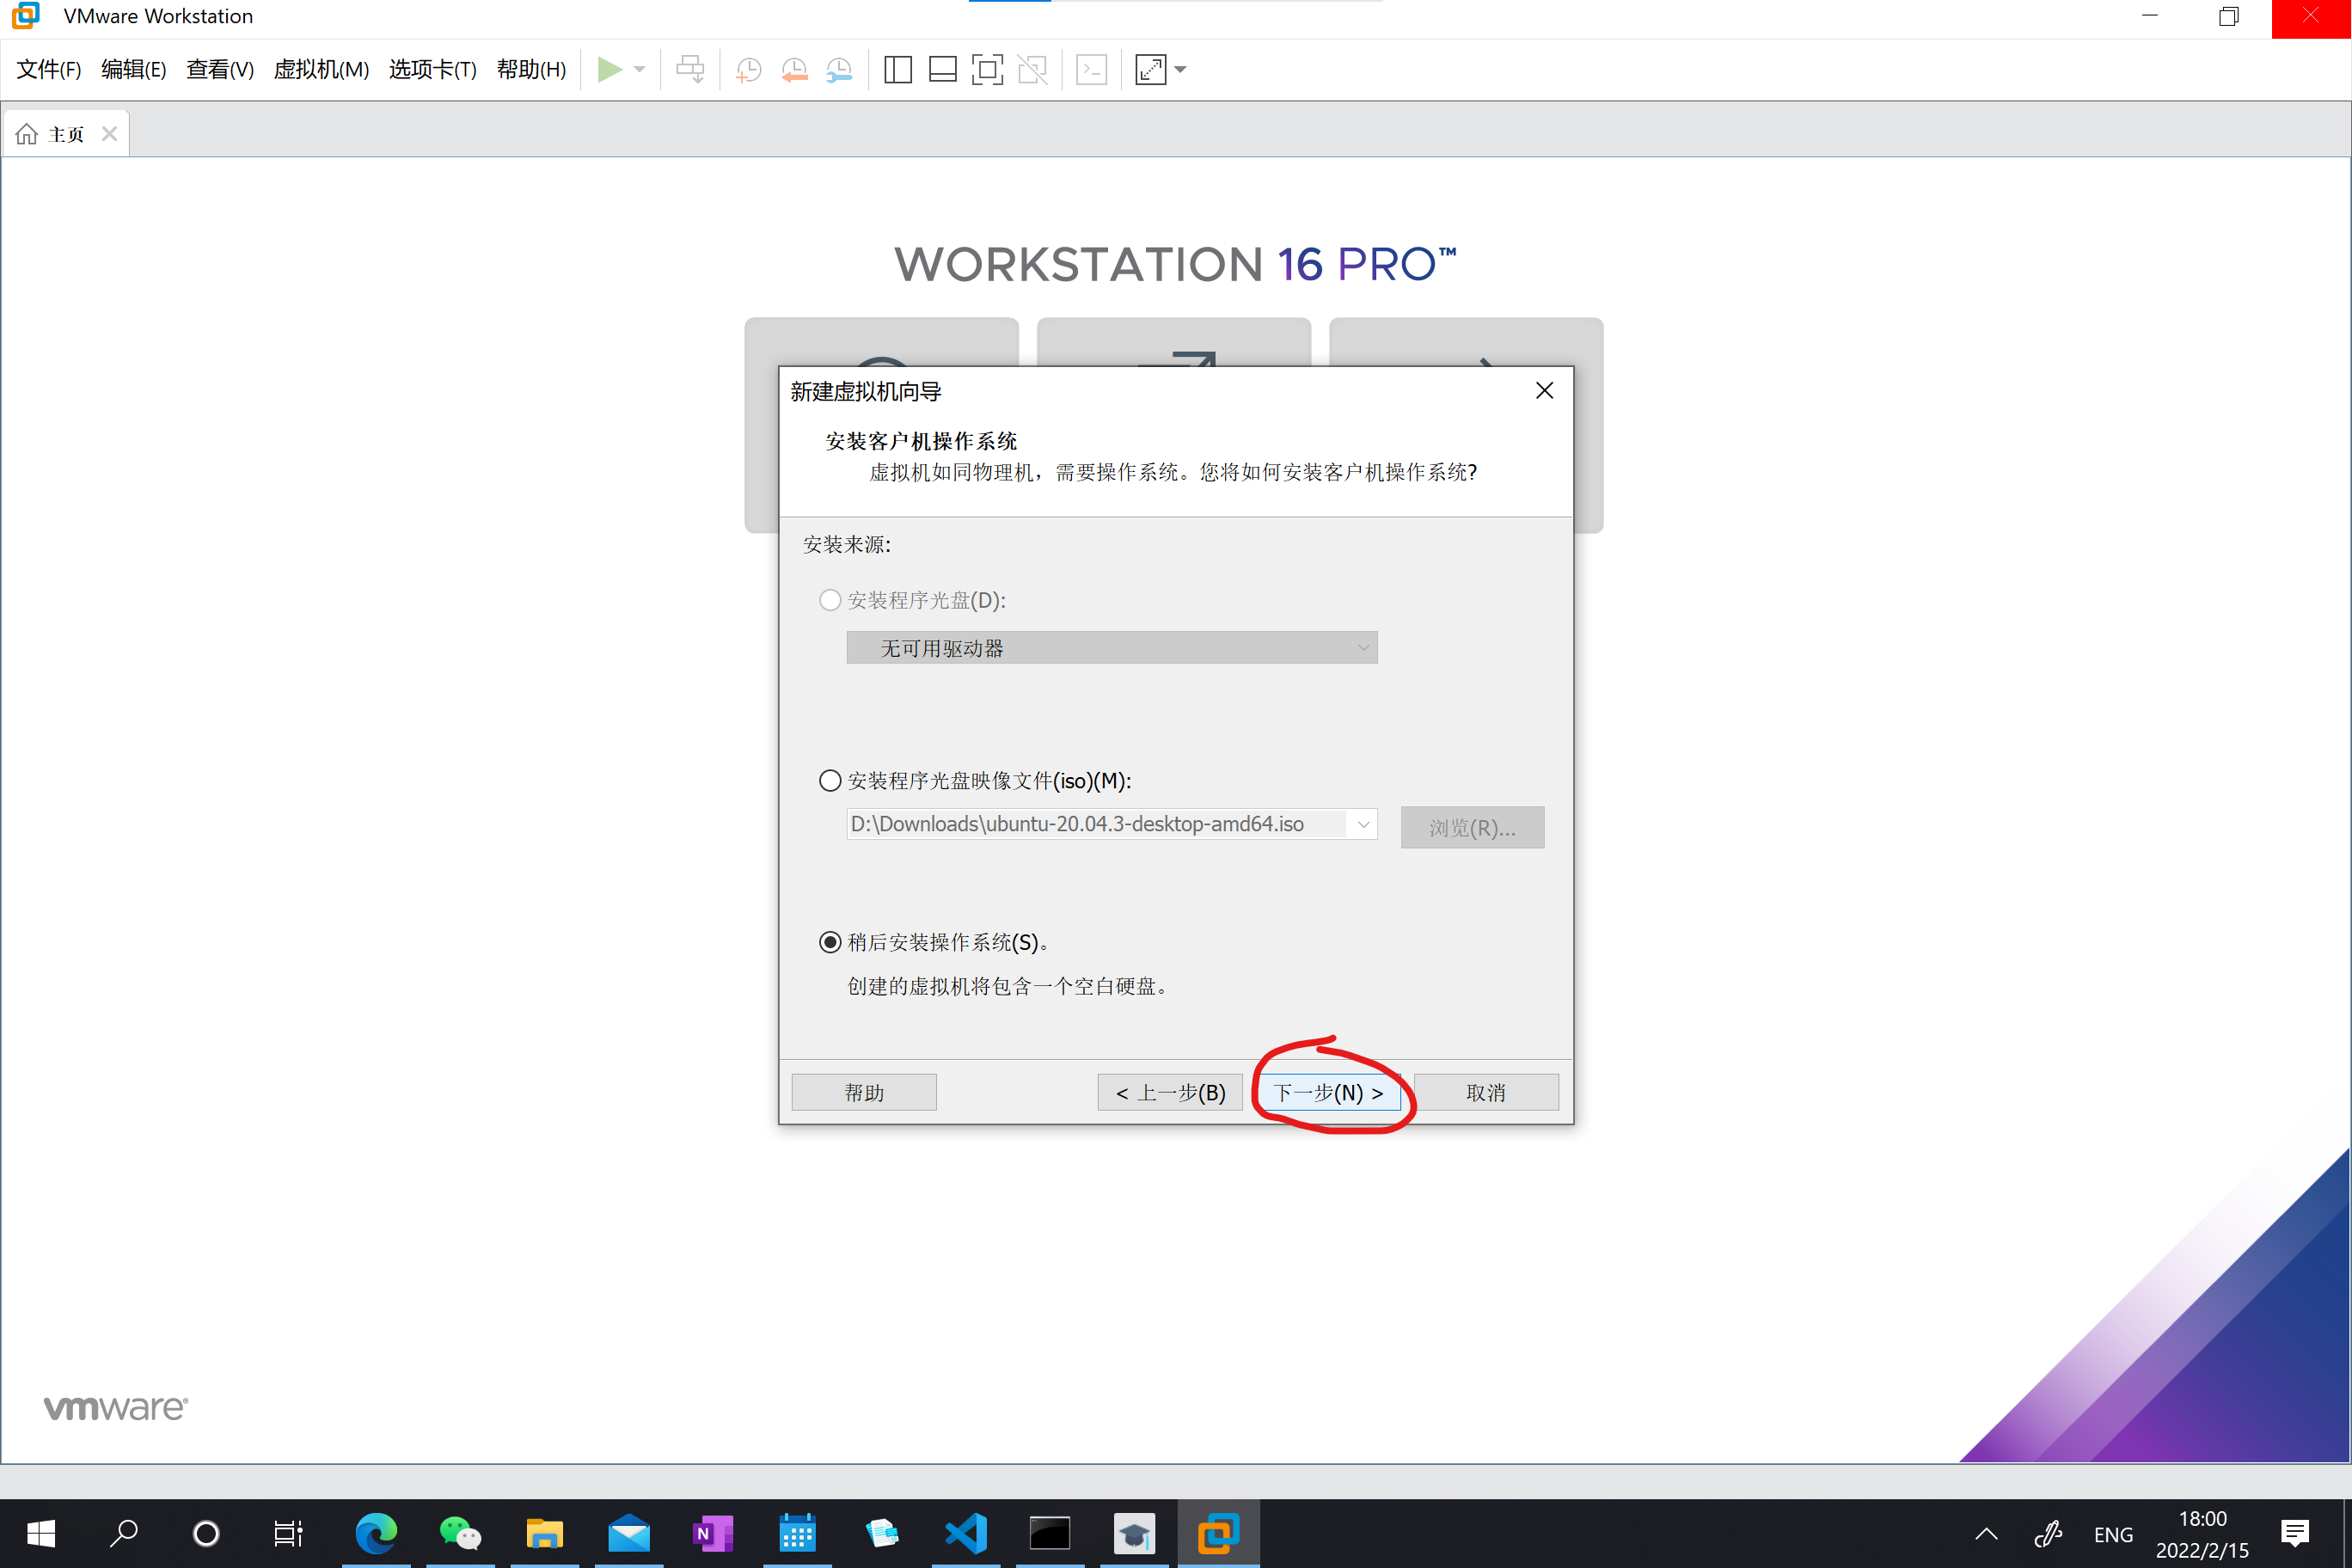
\includegraphics[width=0.8\textwidth]{assets/u5.png}
    \end{figure}
    \begin{figure}[H]
        \centering
        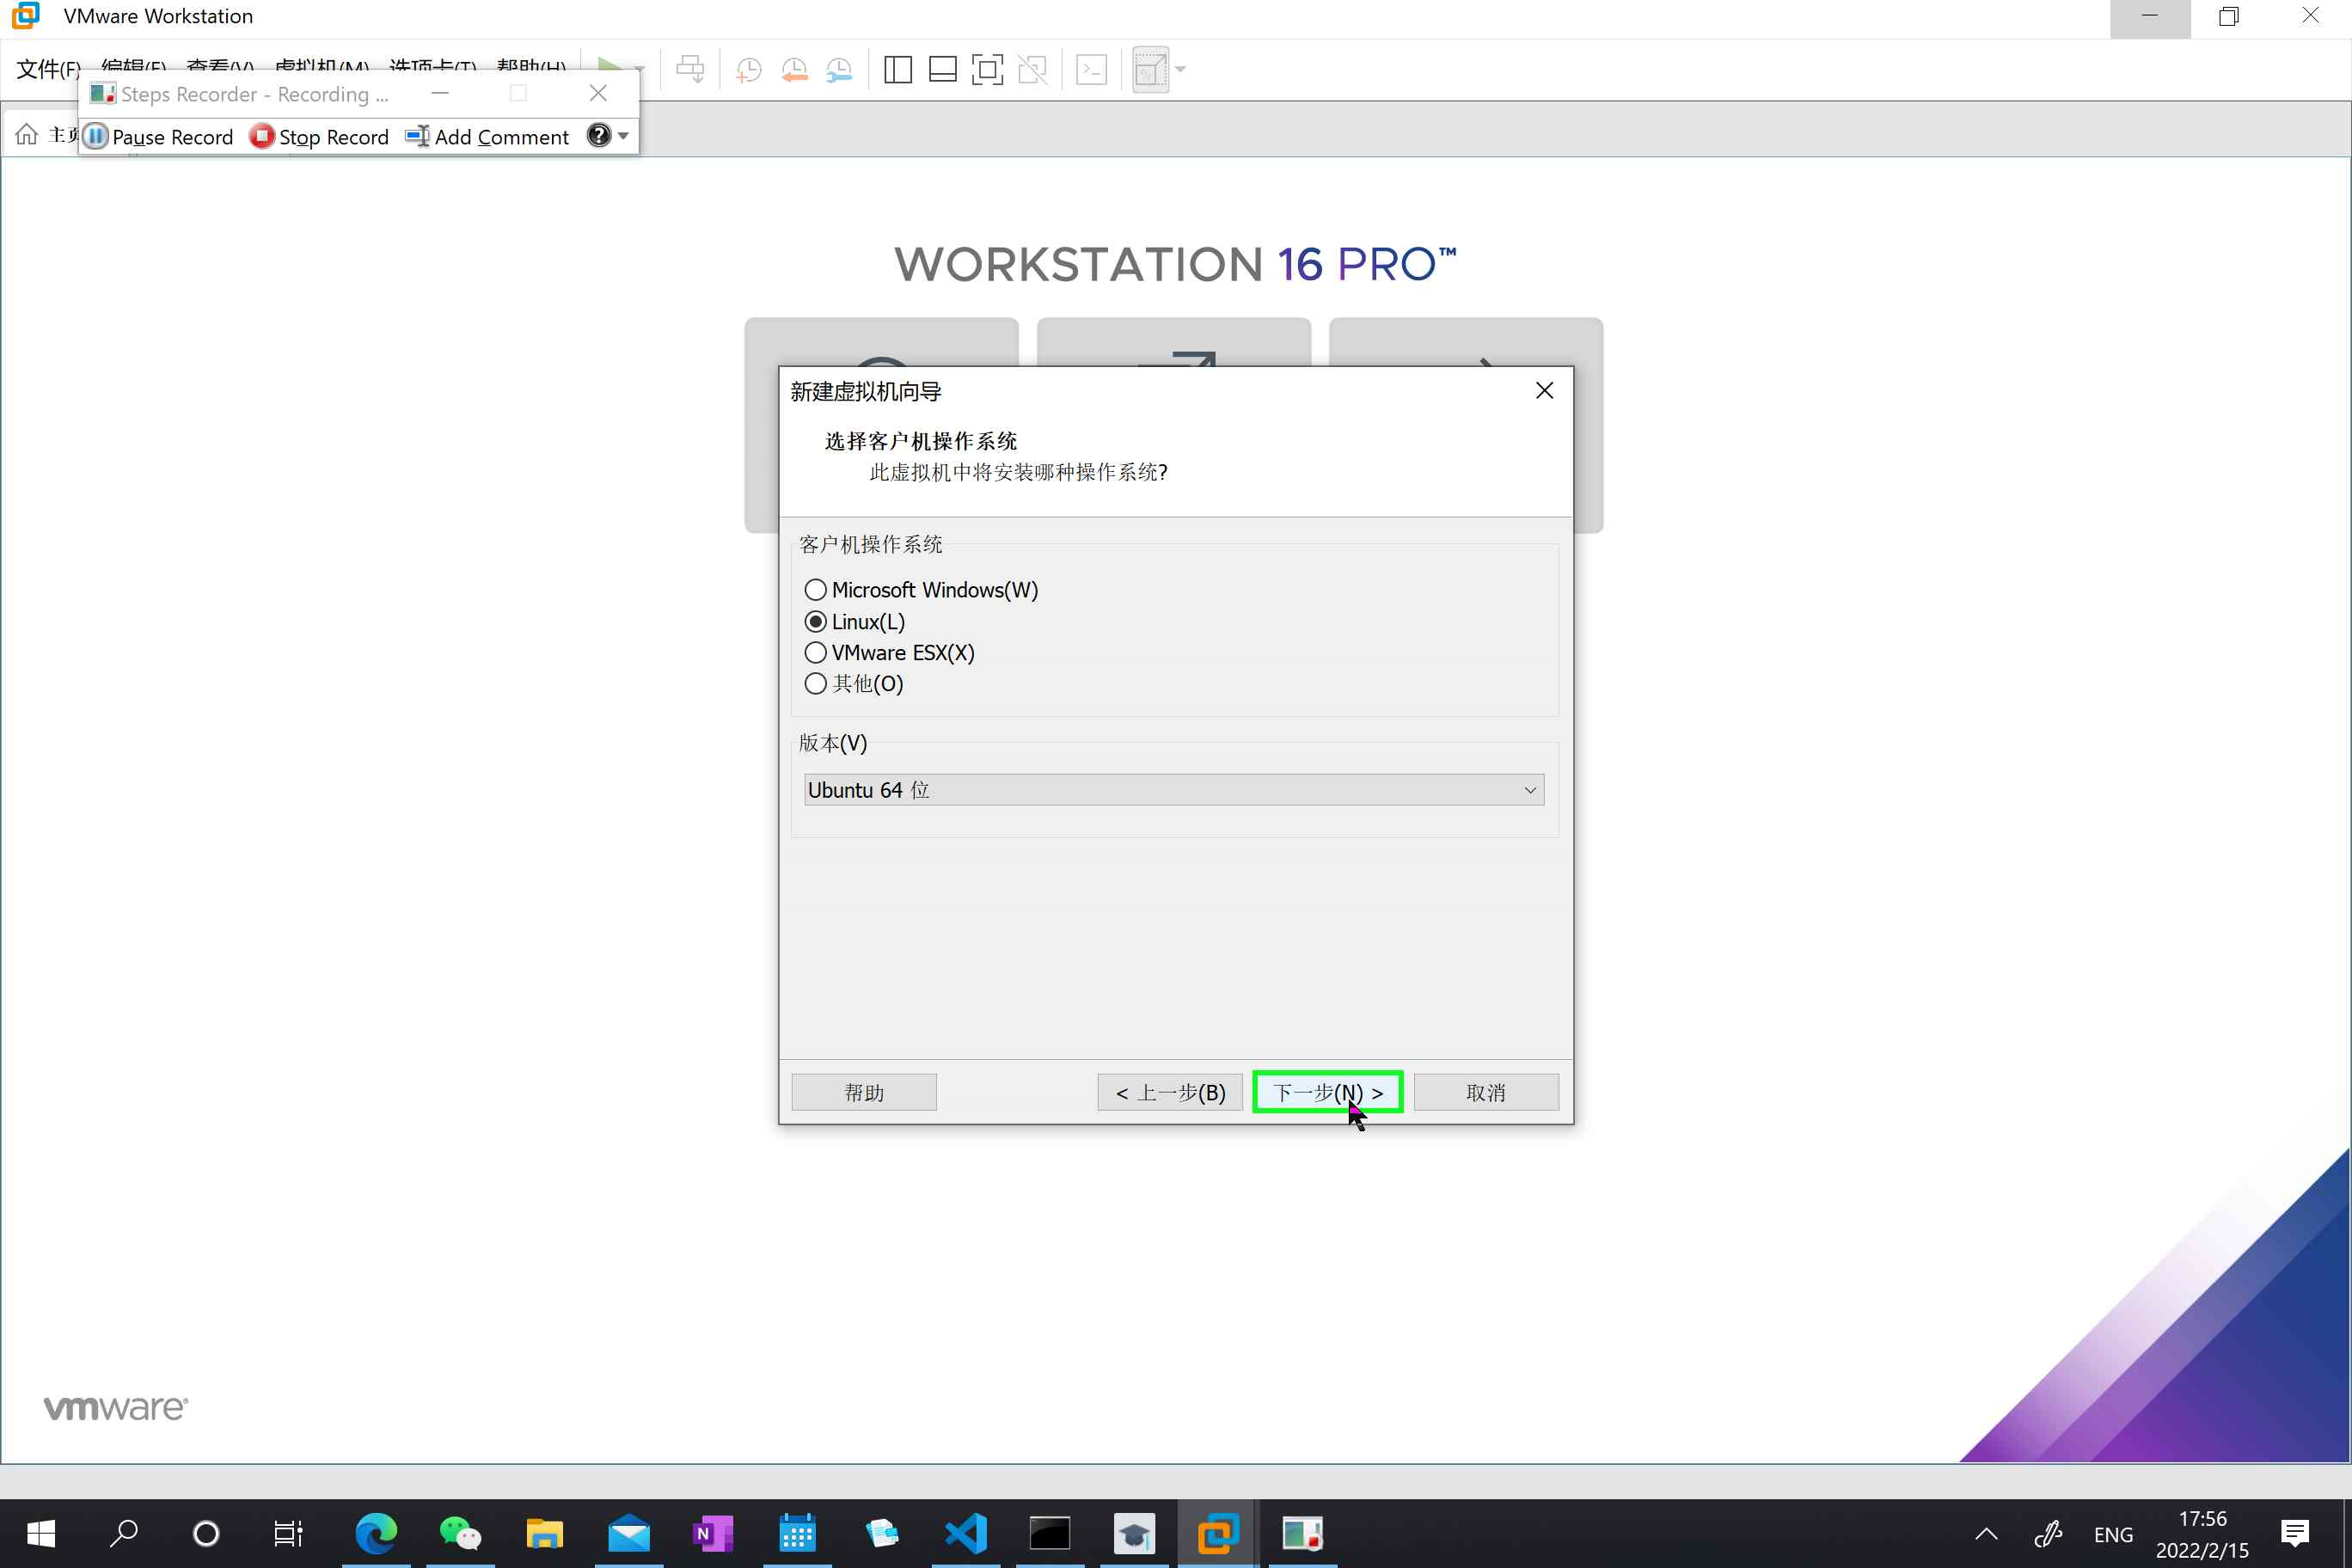
\includegraphics[width=0.8\textwidth]{assets/u6.png}
    \end{figure}
    \begin{figure}[H]
        \centering
        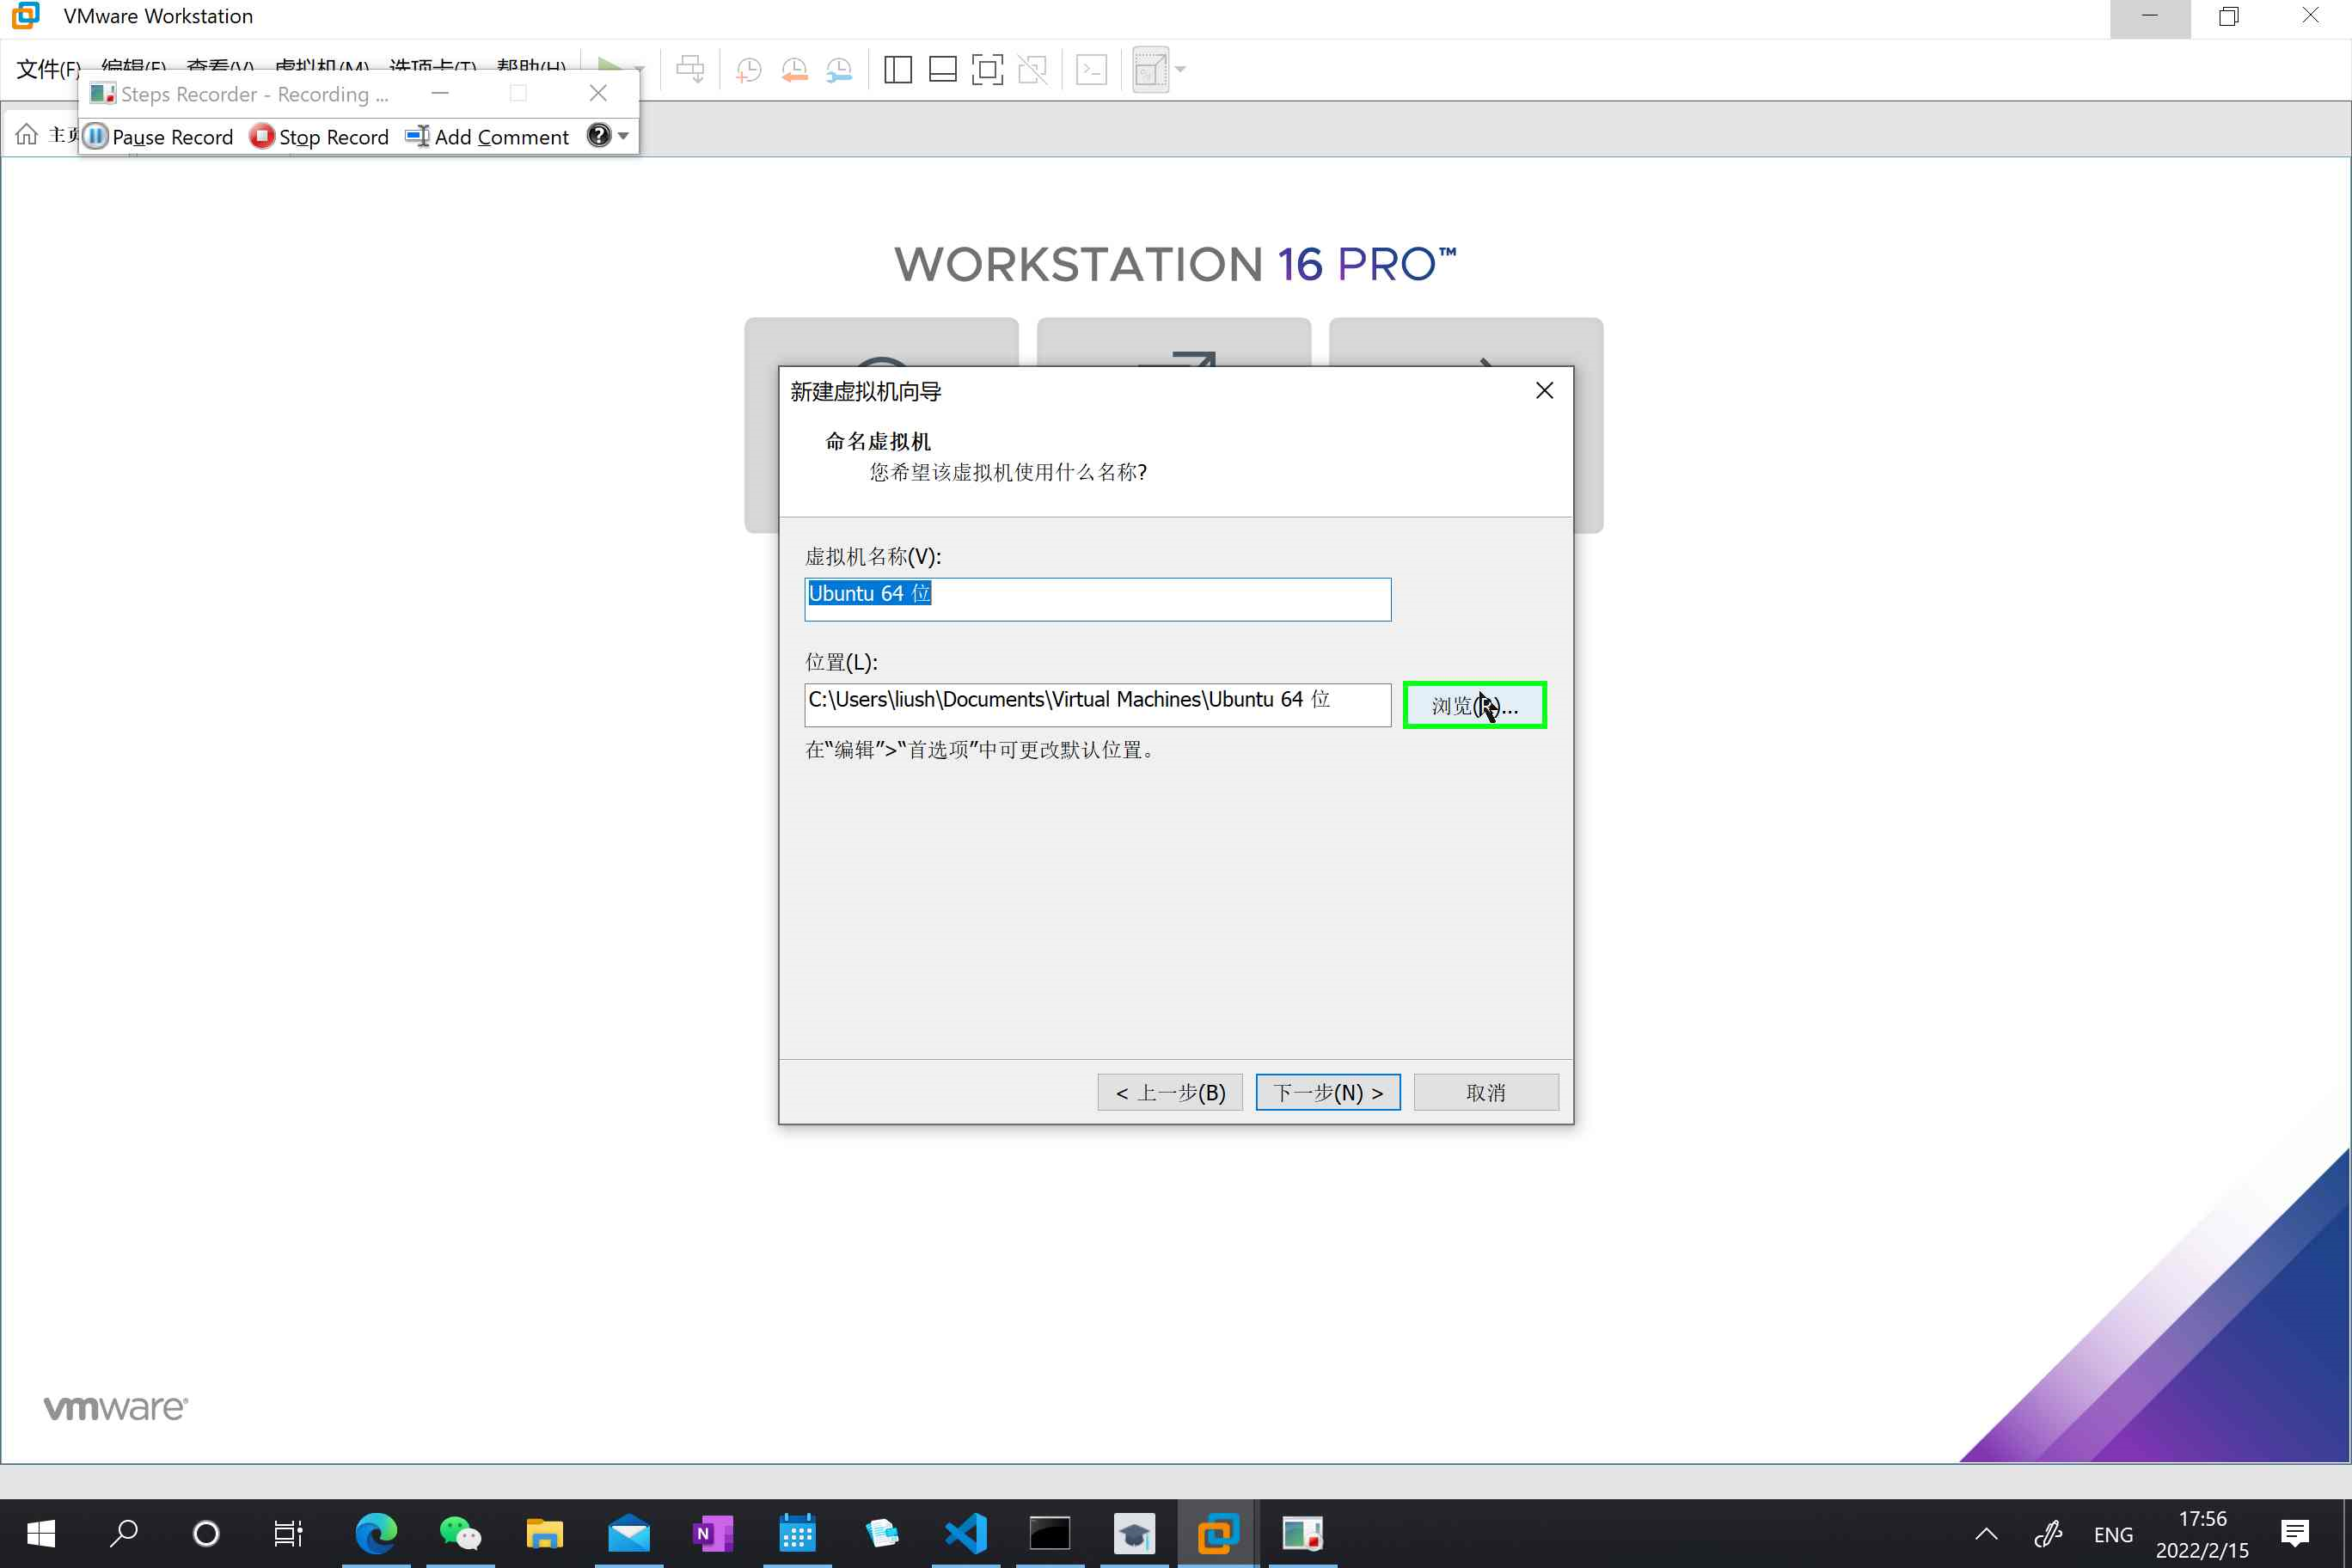
\includegraphics[width=0.8\textwidth]{assets/u7.png}
    \end{figure}
    \begin{figure}[H]
        \centering
        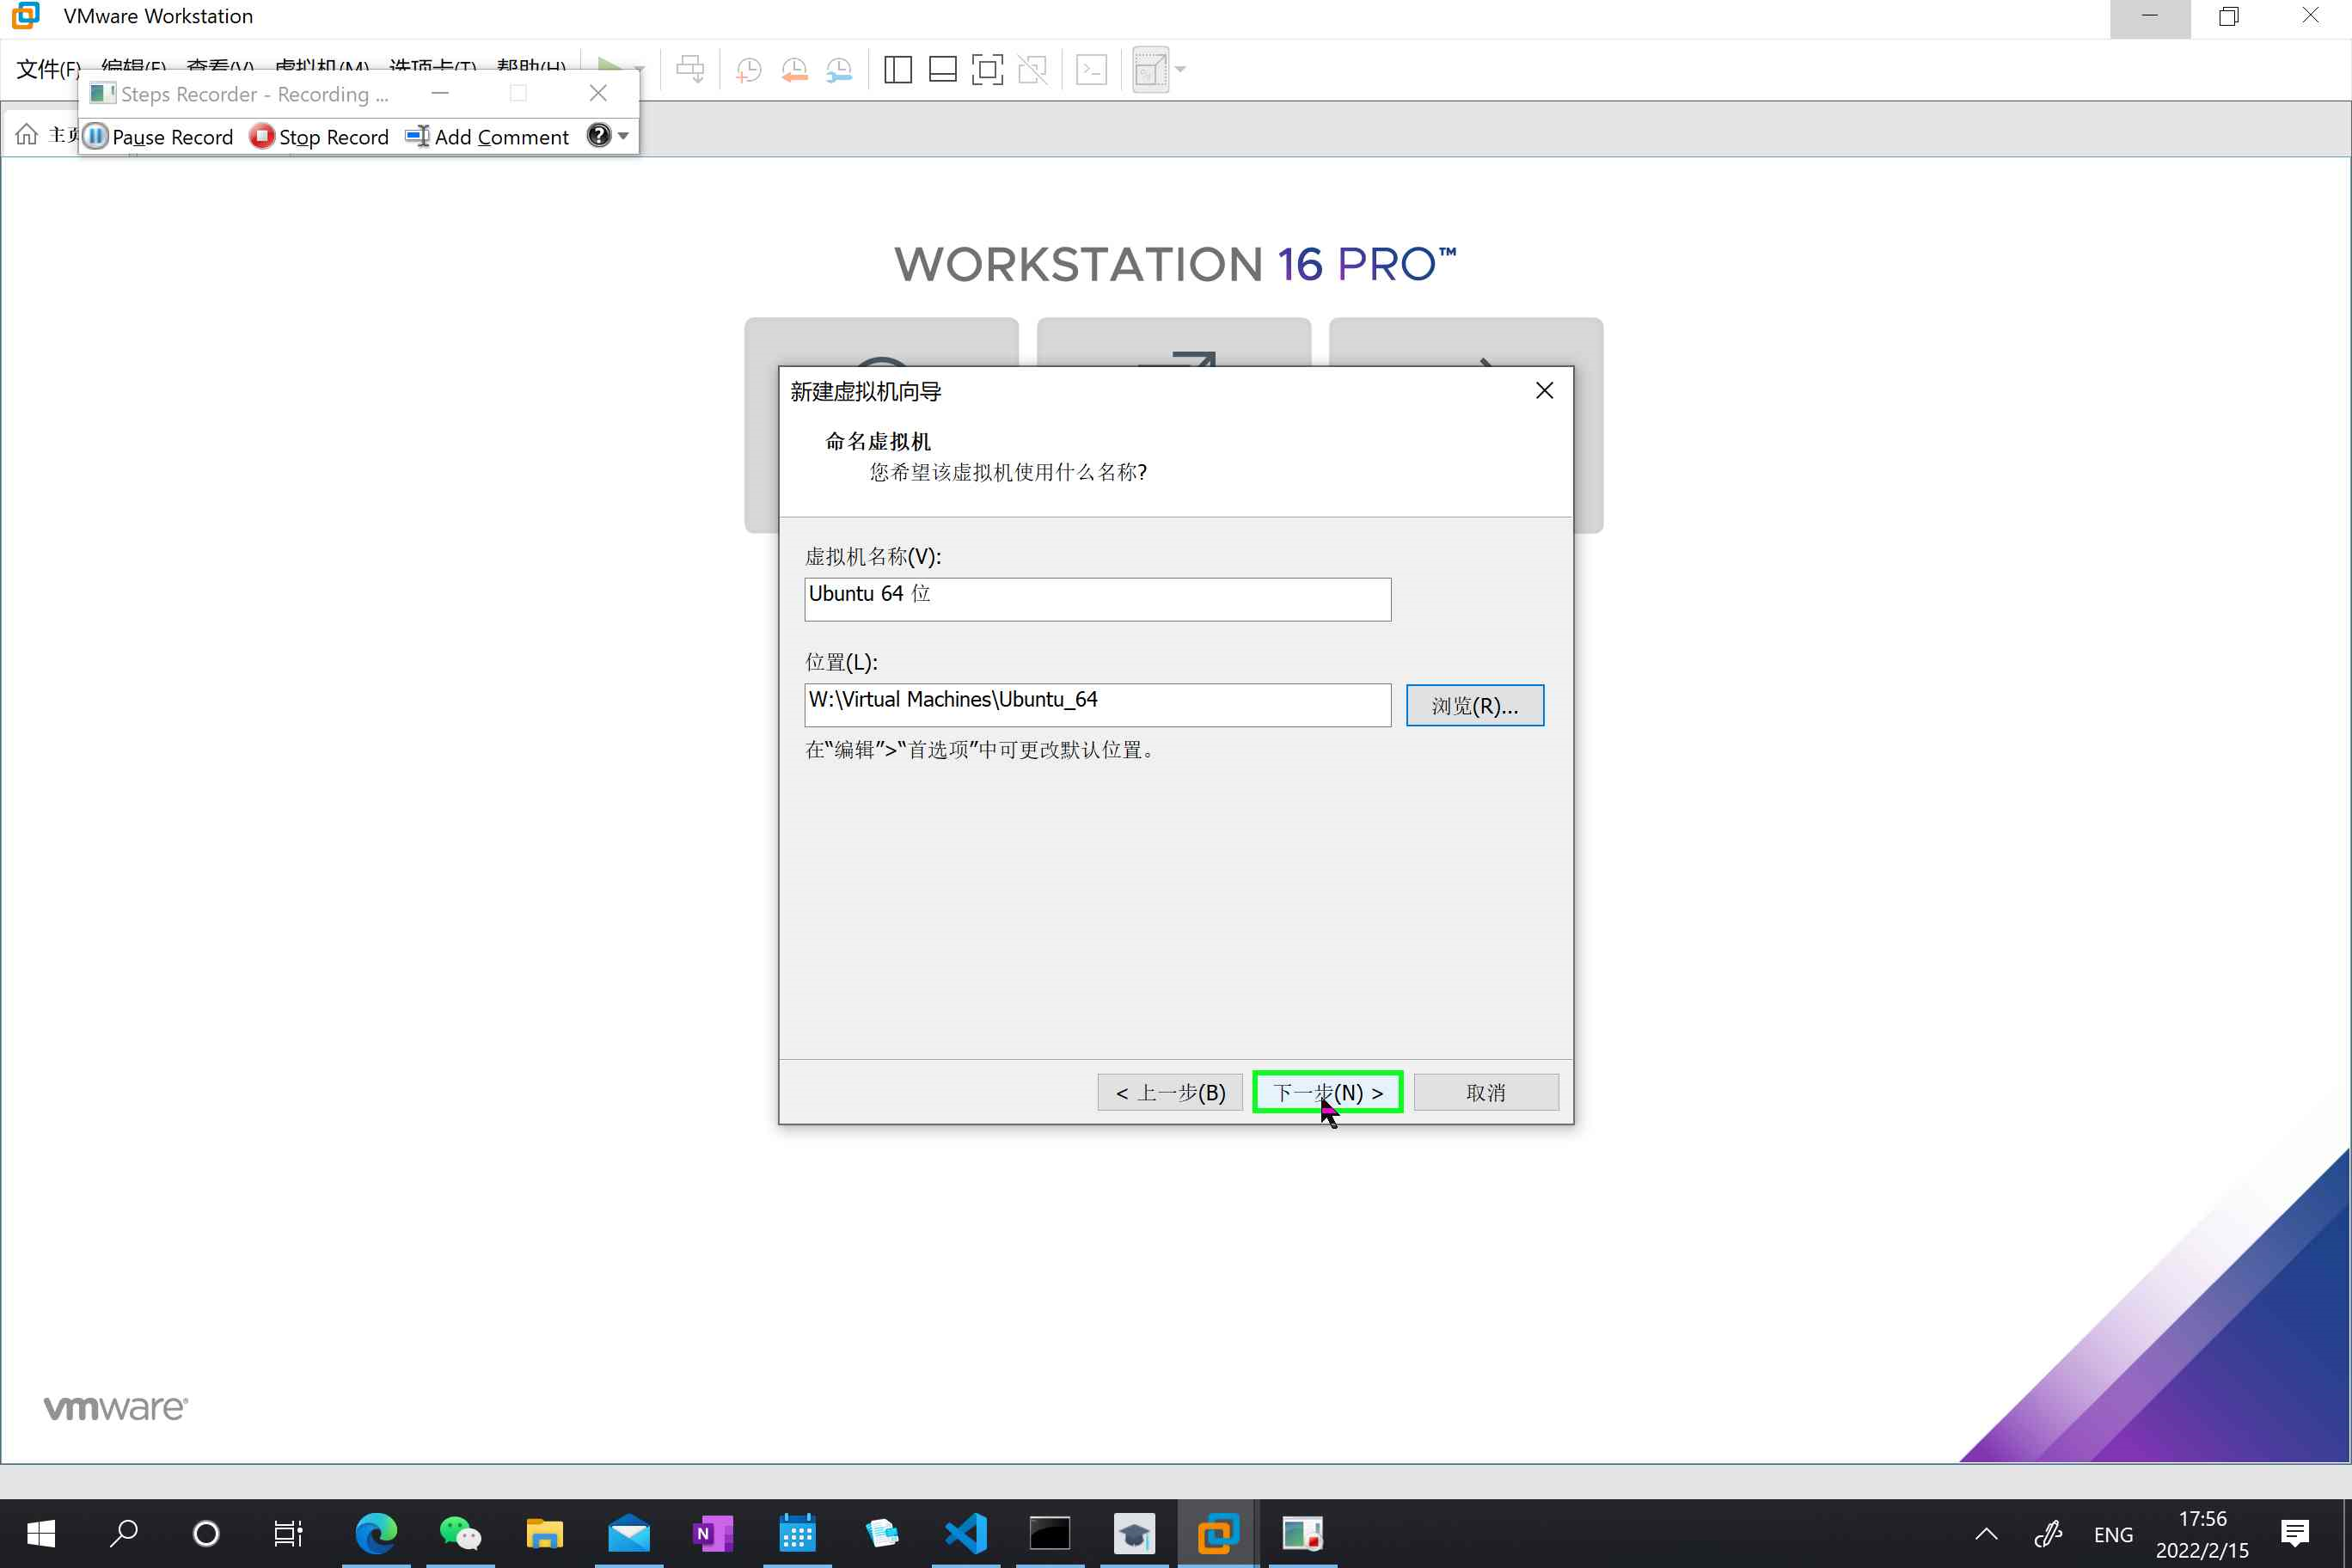
\includegraphics[width=0.8\textwidth]{assets/u8.png}
    \end{figure}
    \begin{figure}[H]
        \centering
        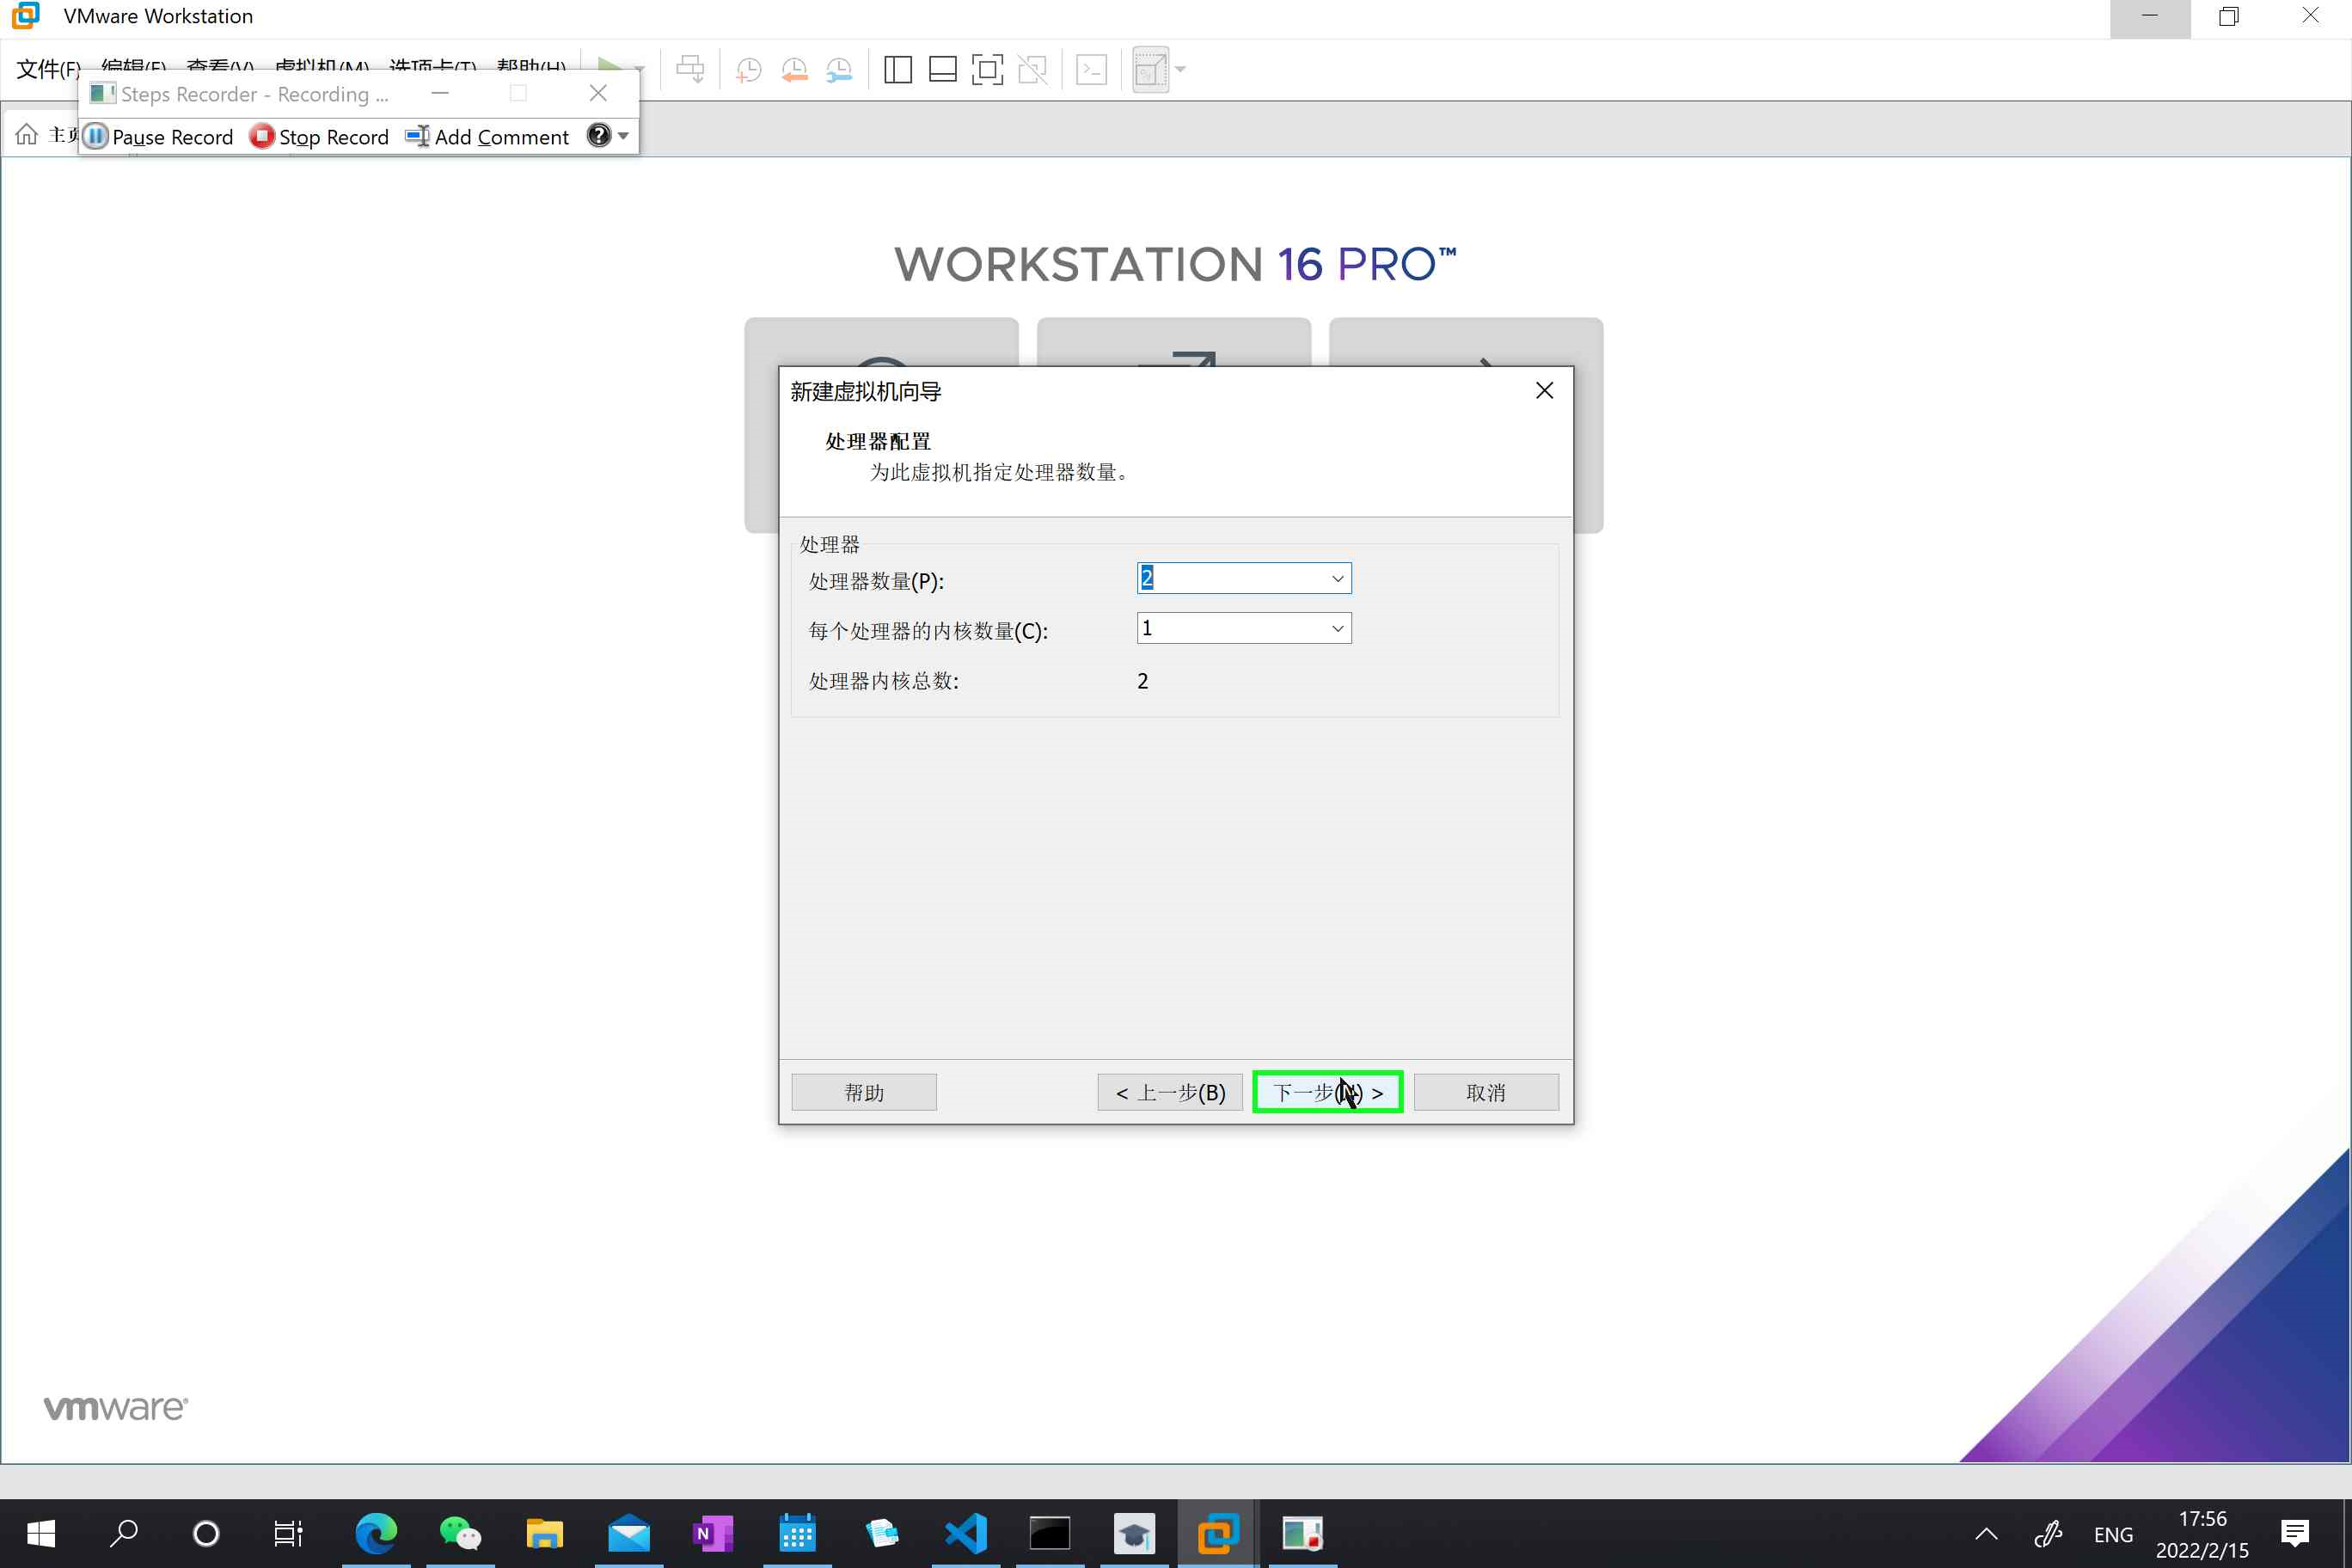
\includegraphics[width=0.8\textwidth]{assets/u9.png}
    \end{figure}
    \begin{figure}[H]
        \centering
        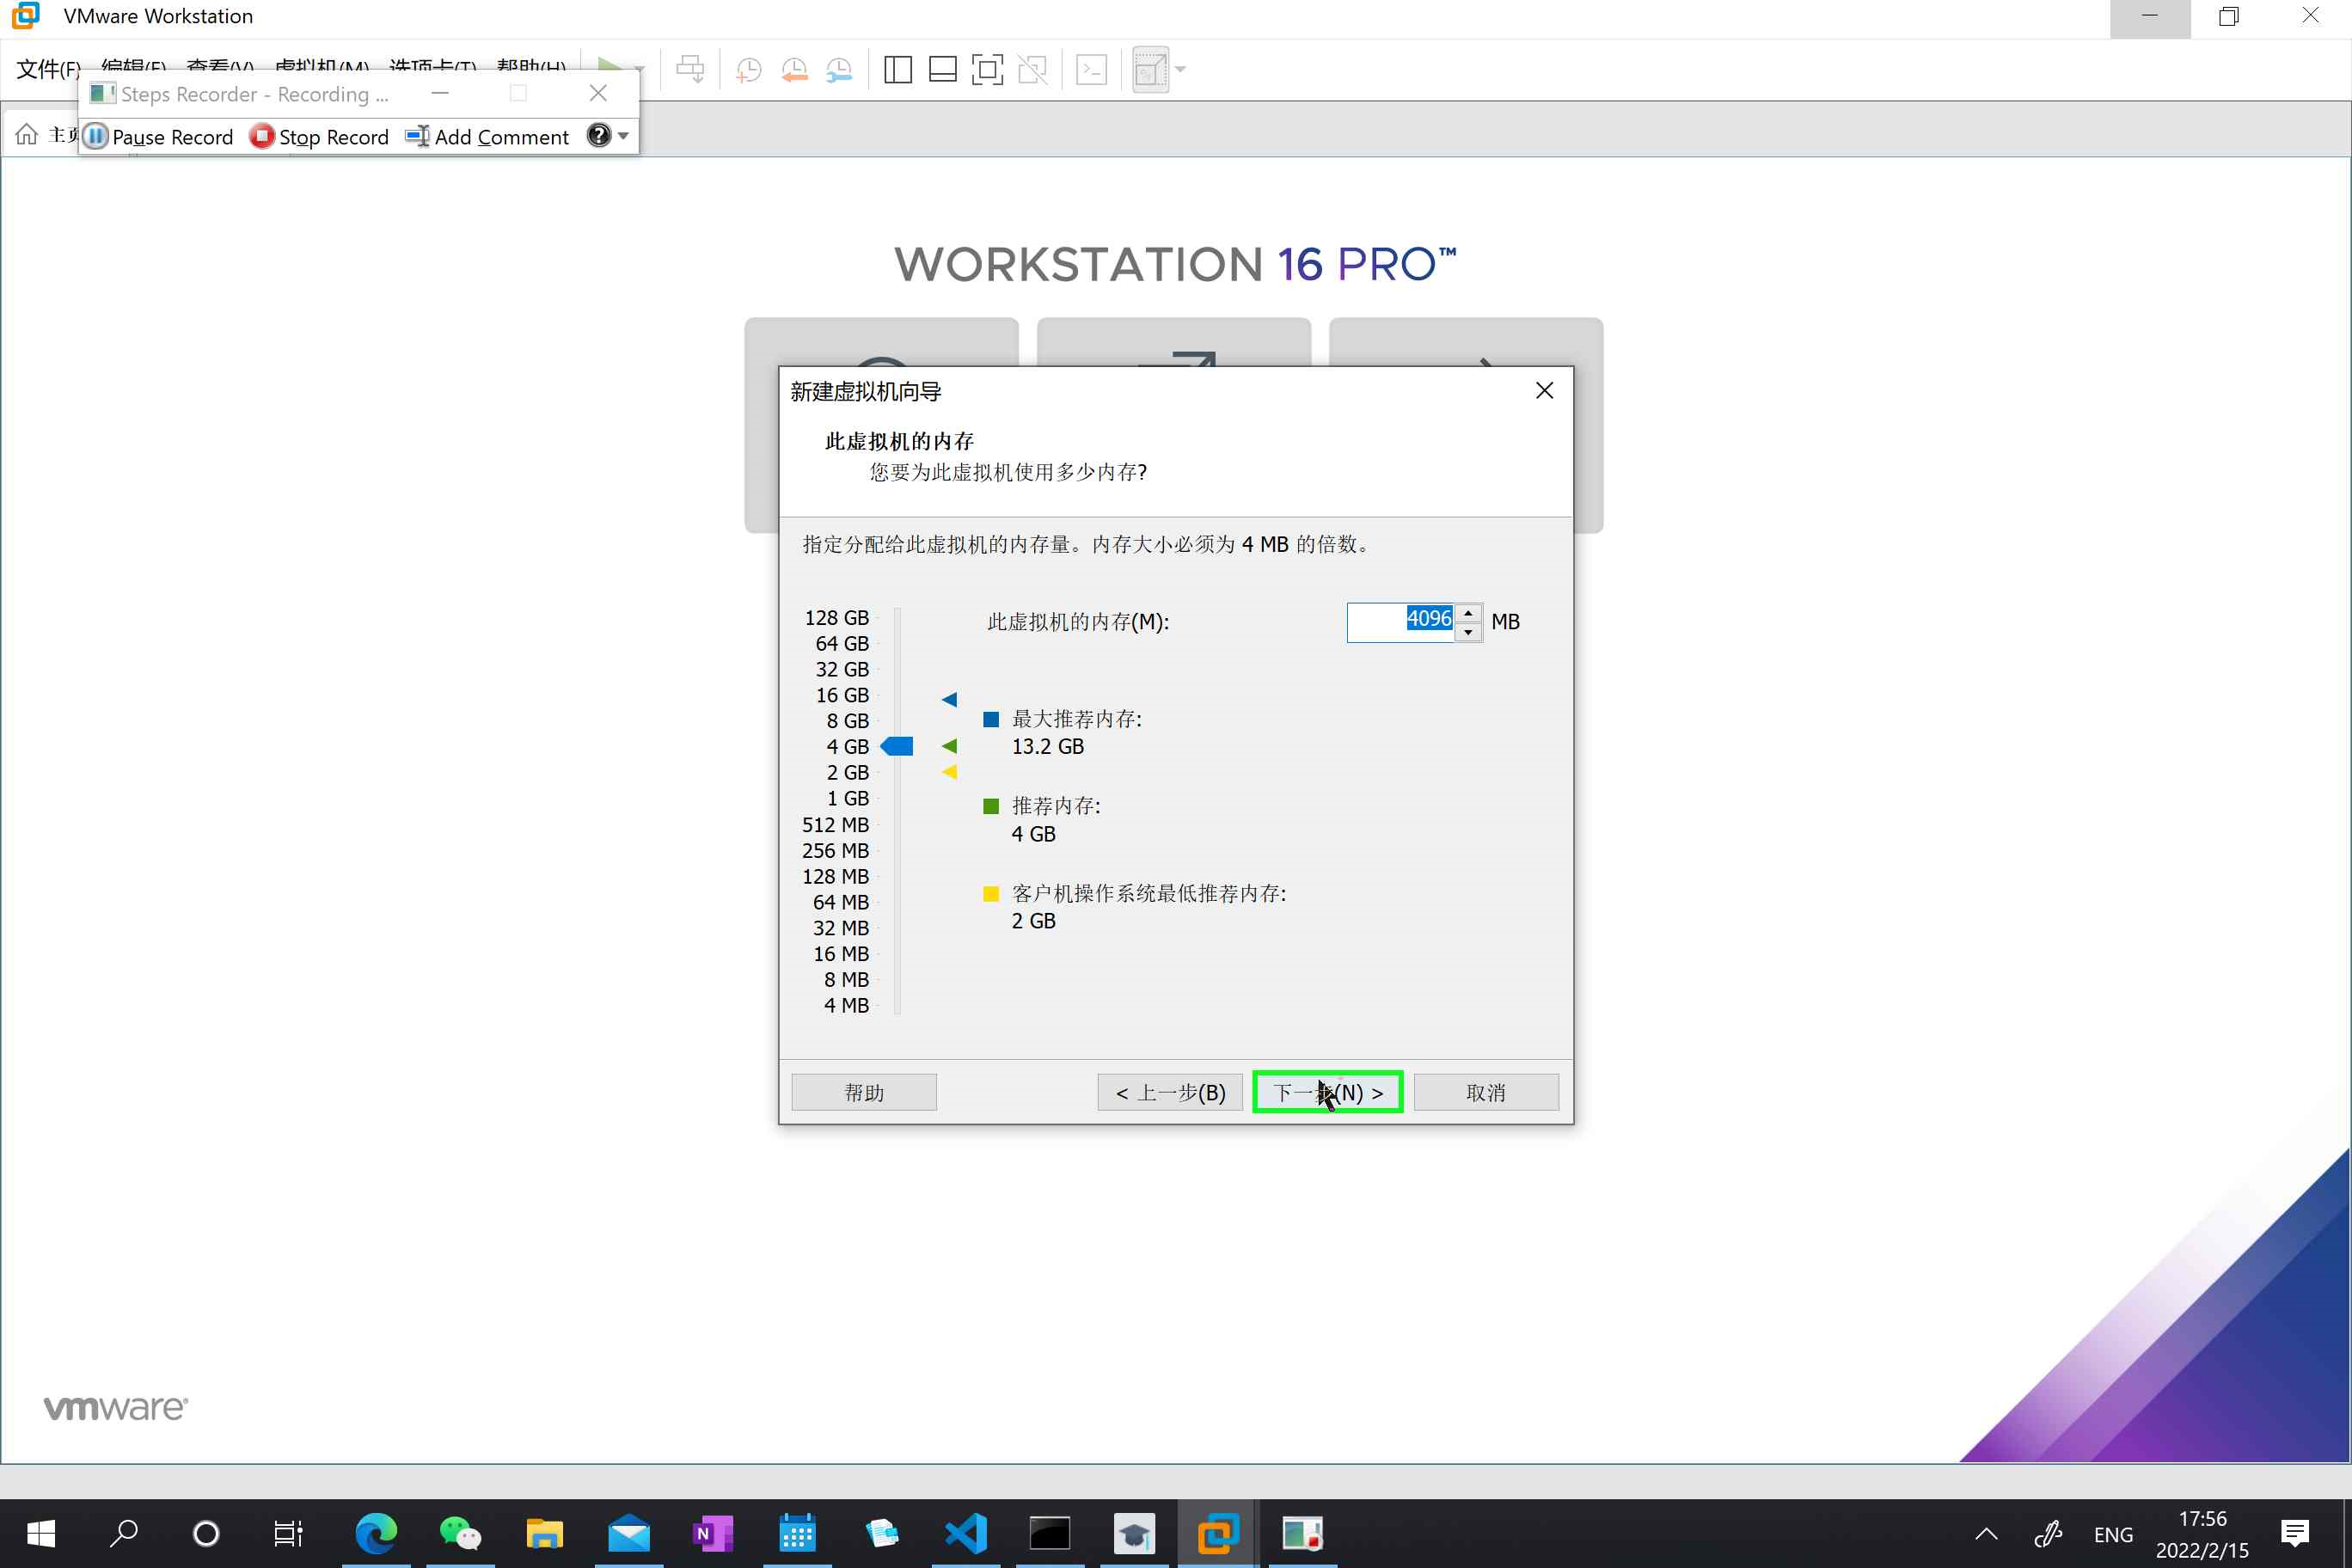
\includegraphics[width=0.8\textwidth]{assets/u11.png}
    \end{figure}
    \begin{figure}[H]
        \centering
        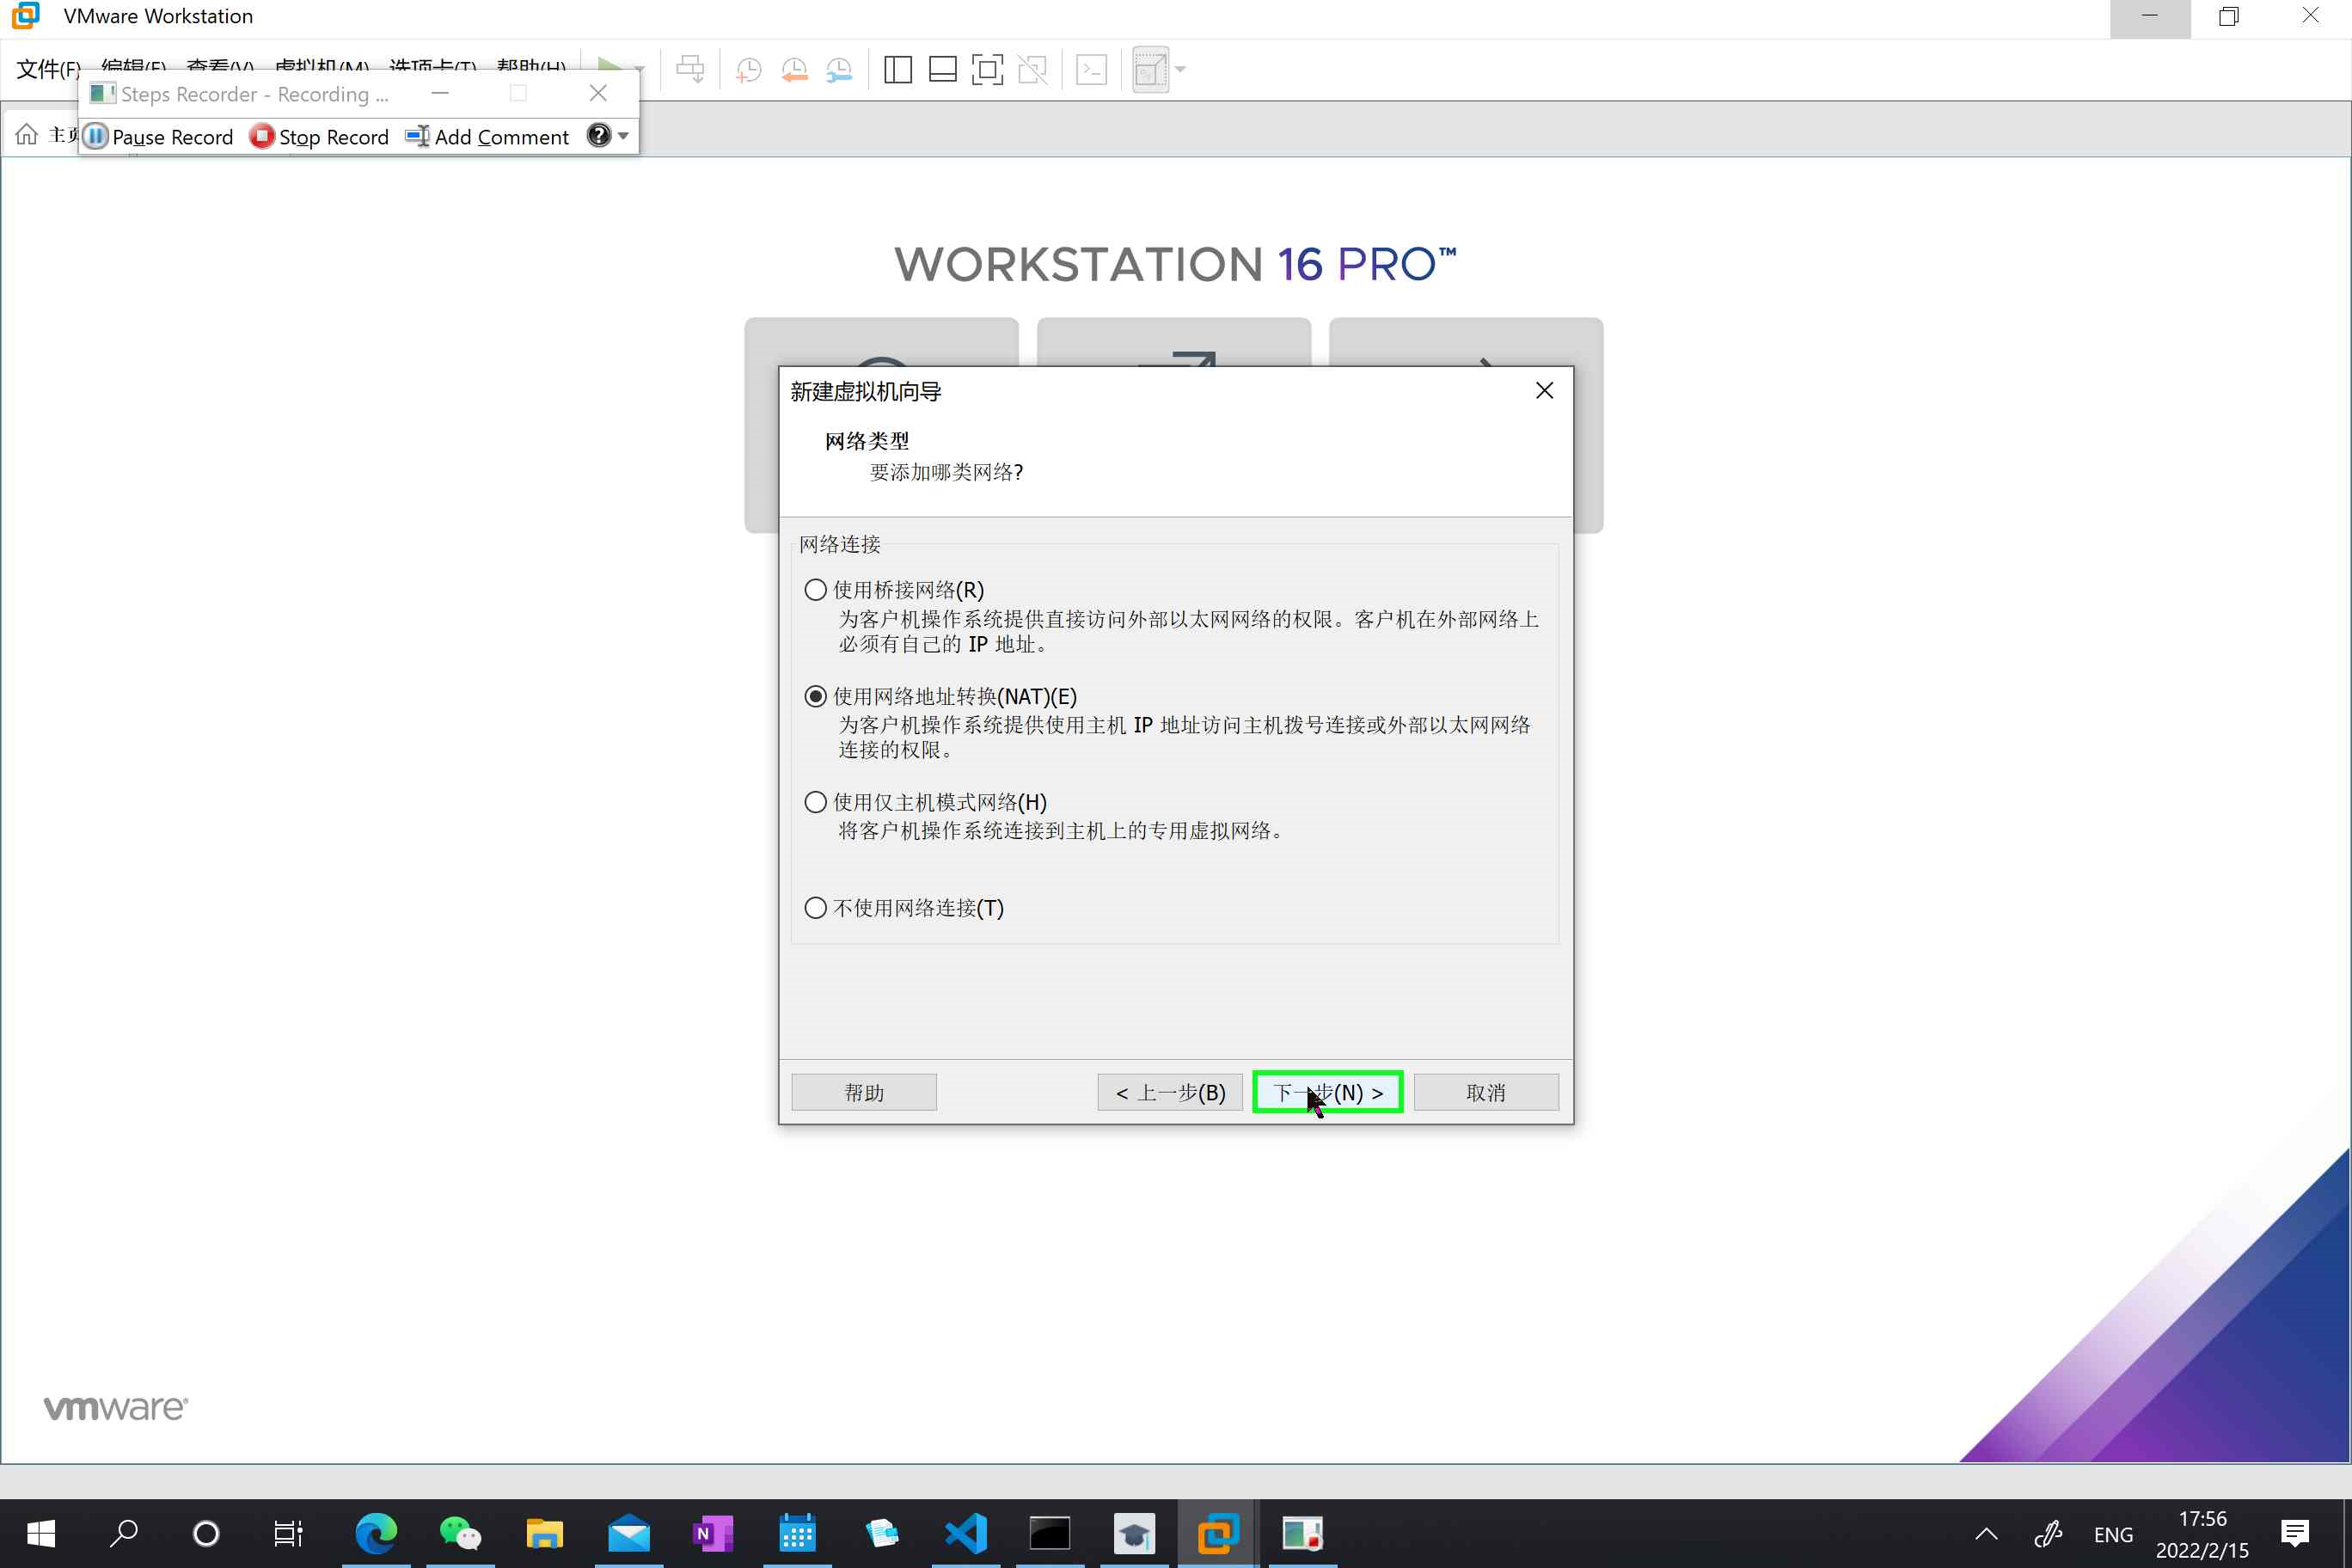
\includegraphics[width=0.8\textwidth]{assets/u12.png}
    \end{figure}
    \begin{figure}[H]
        \centering
        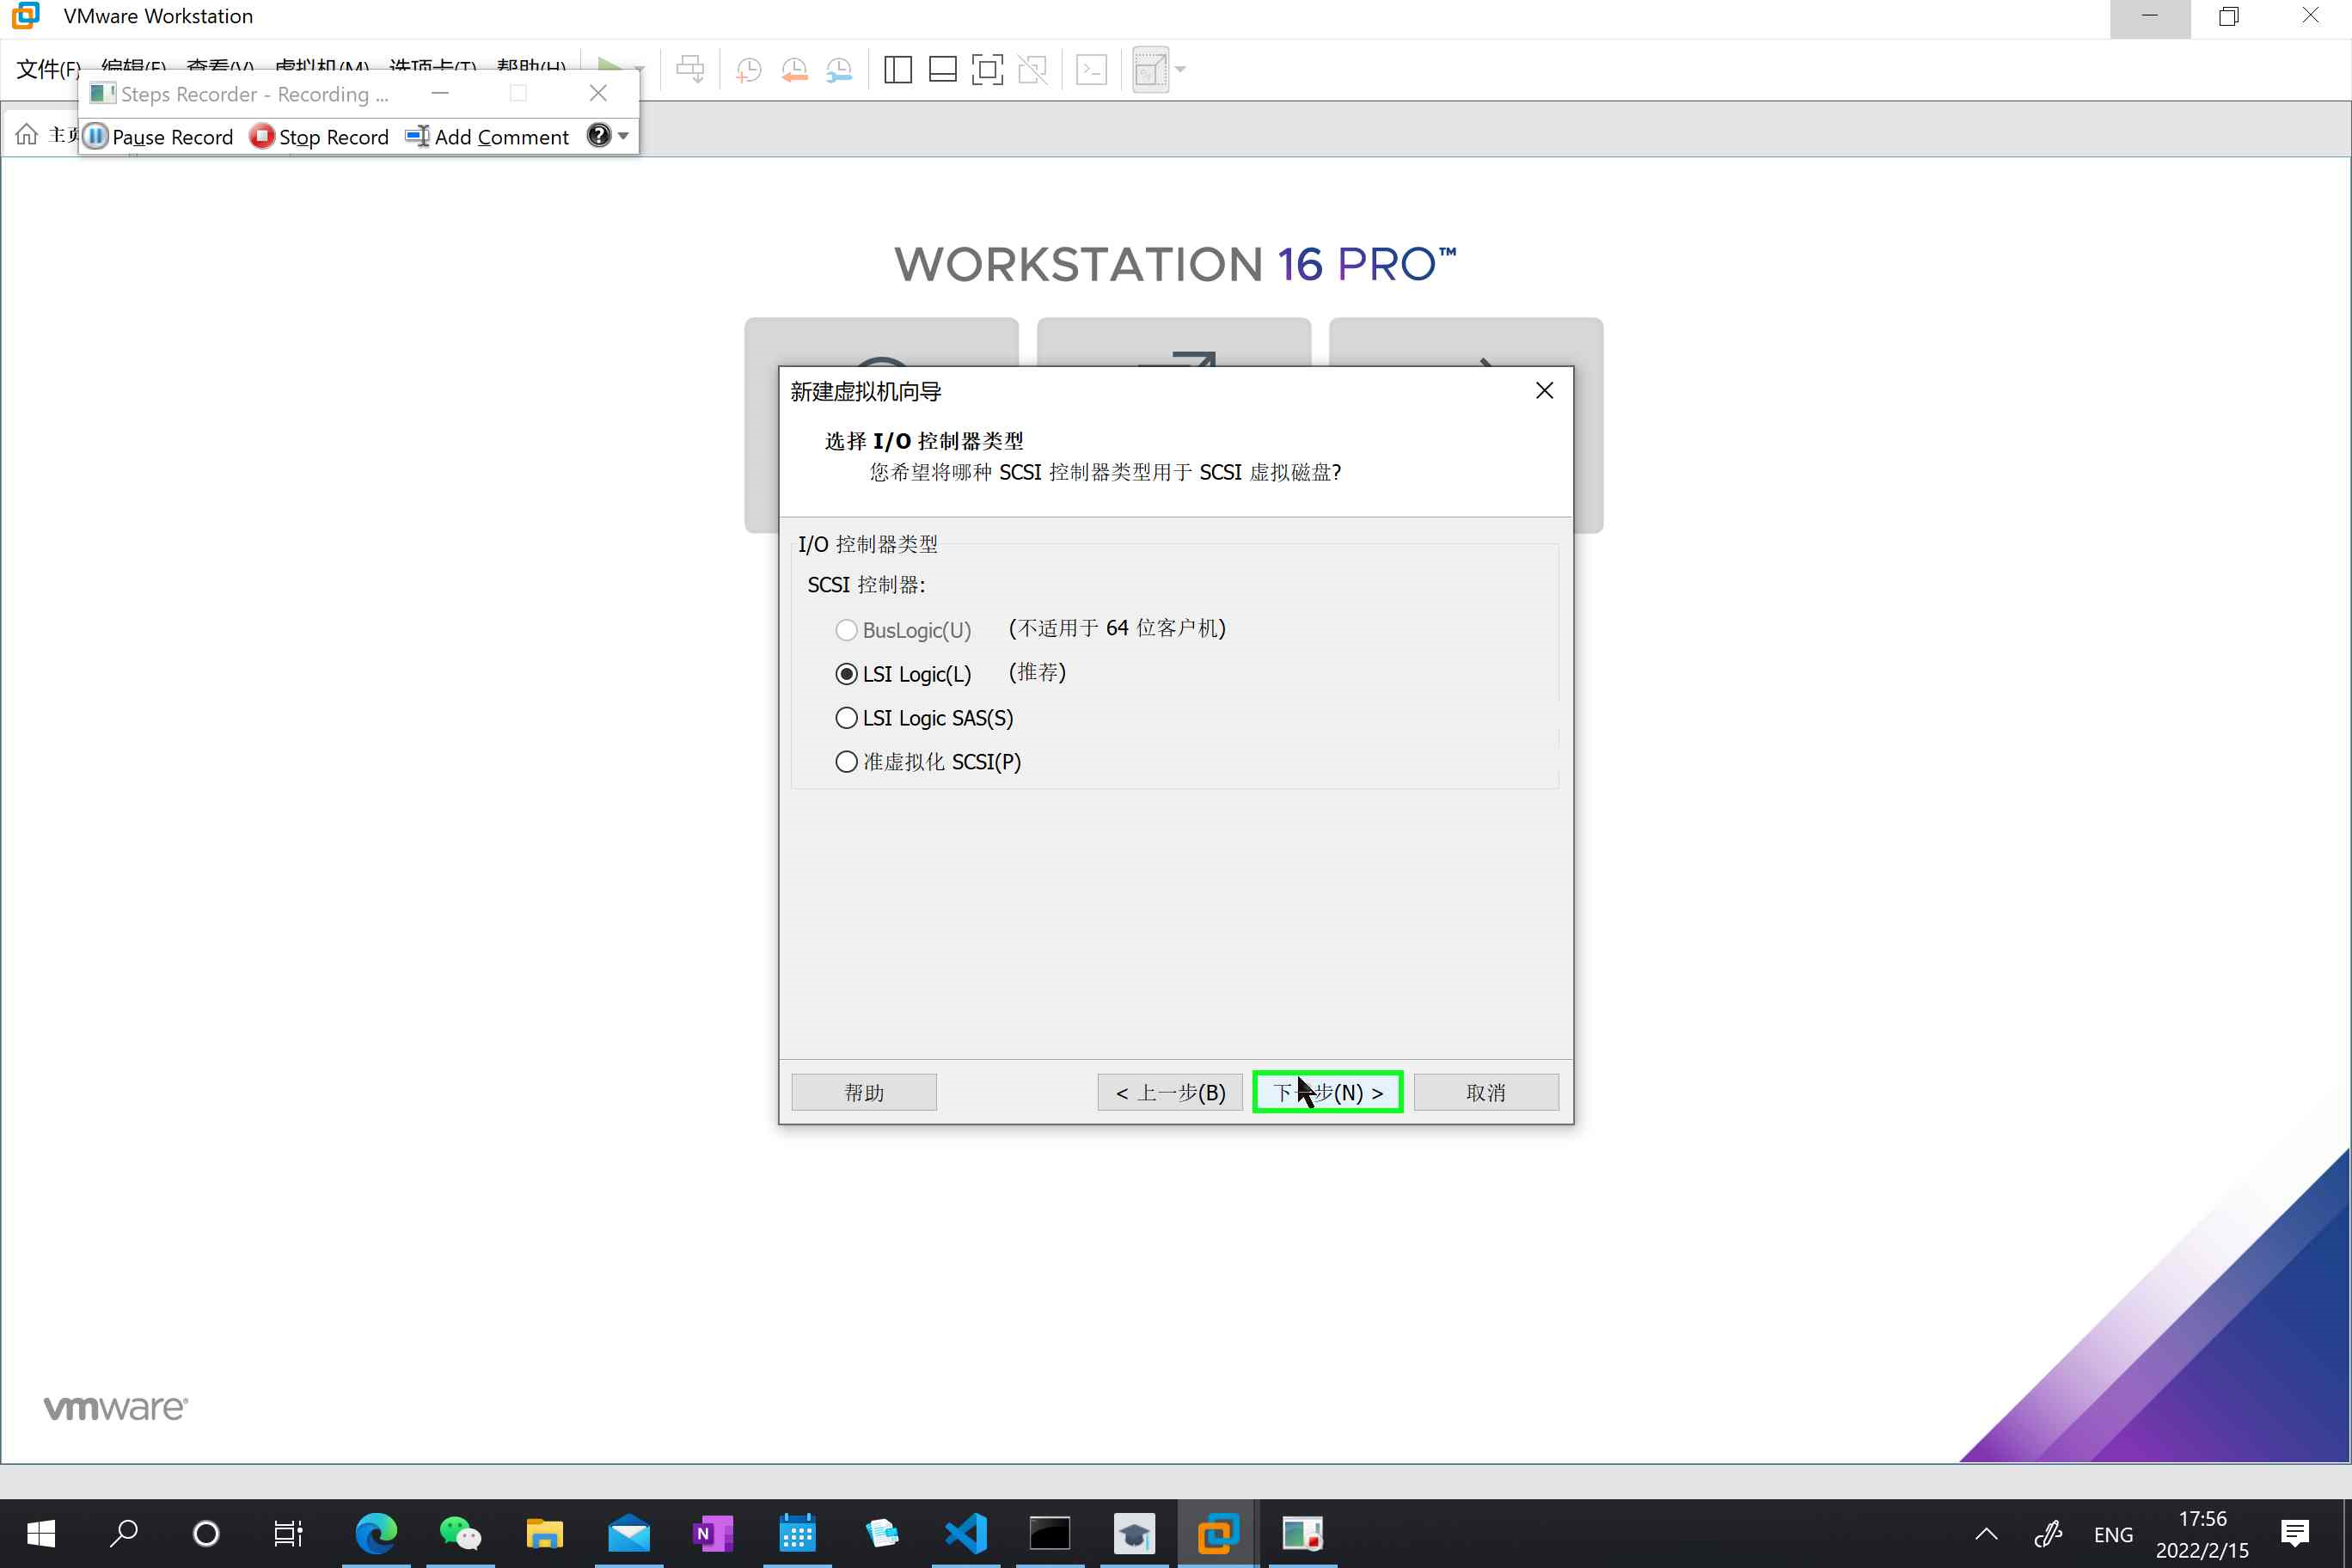
\includegraphics[width=0.8\textwidth]{assets/u13.png}
    \end{figure}
    \begin{figure}[H]
        \centering
        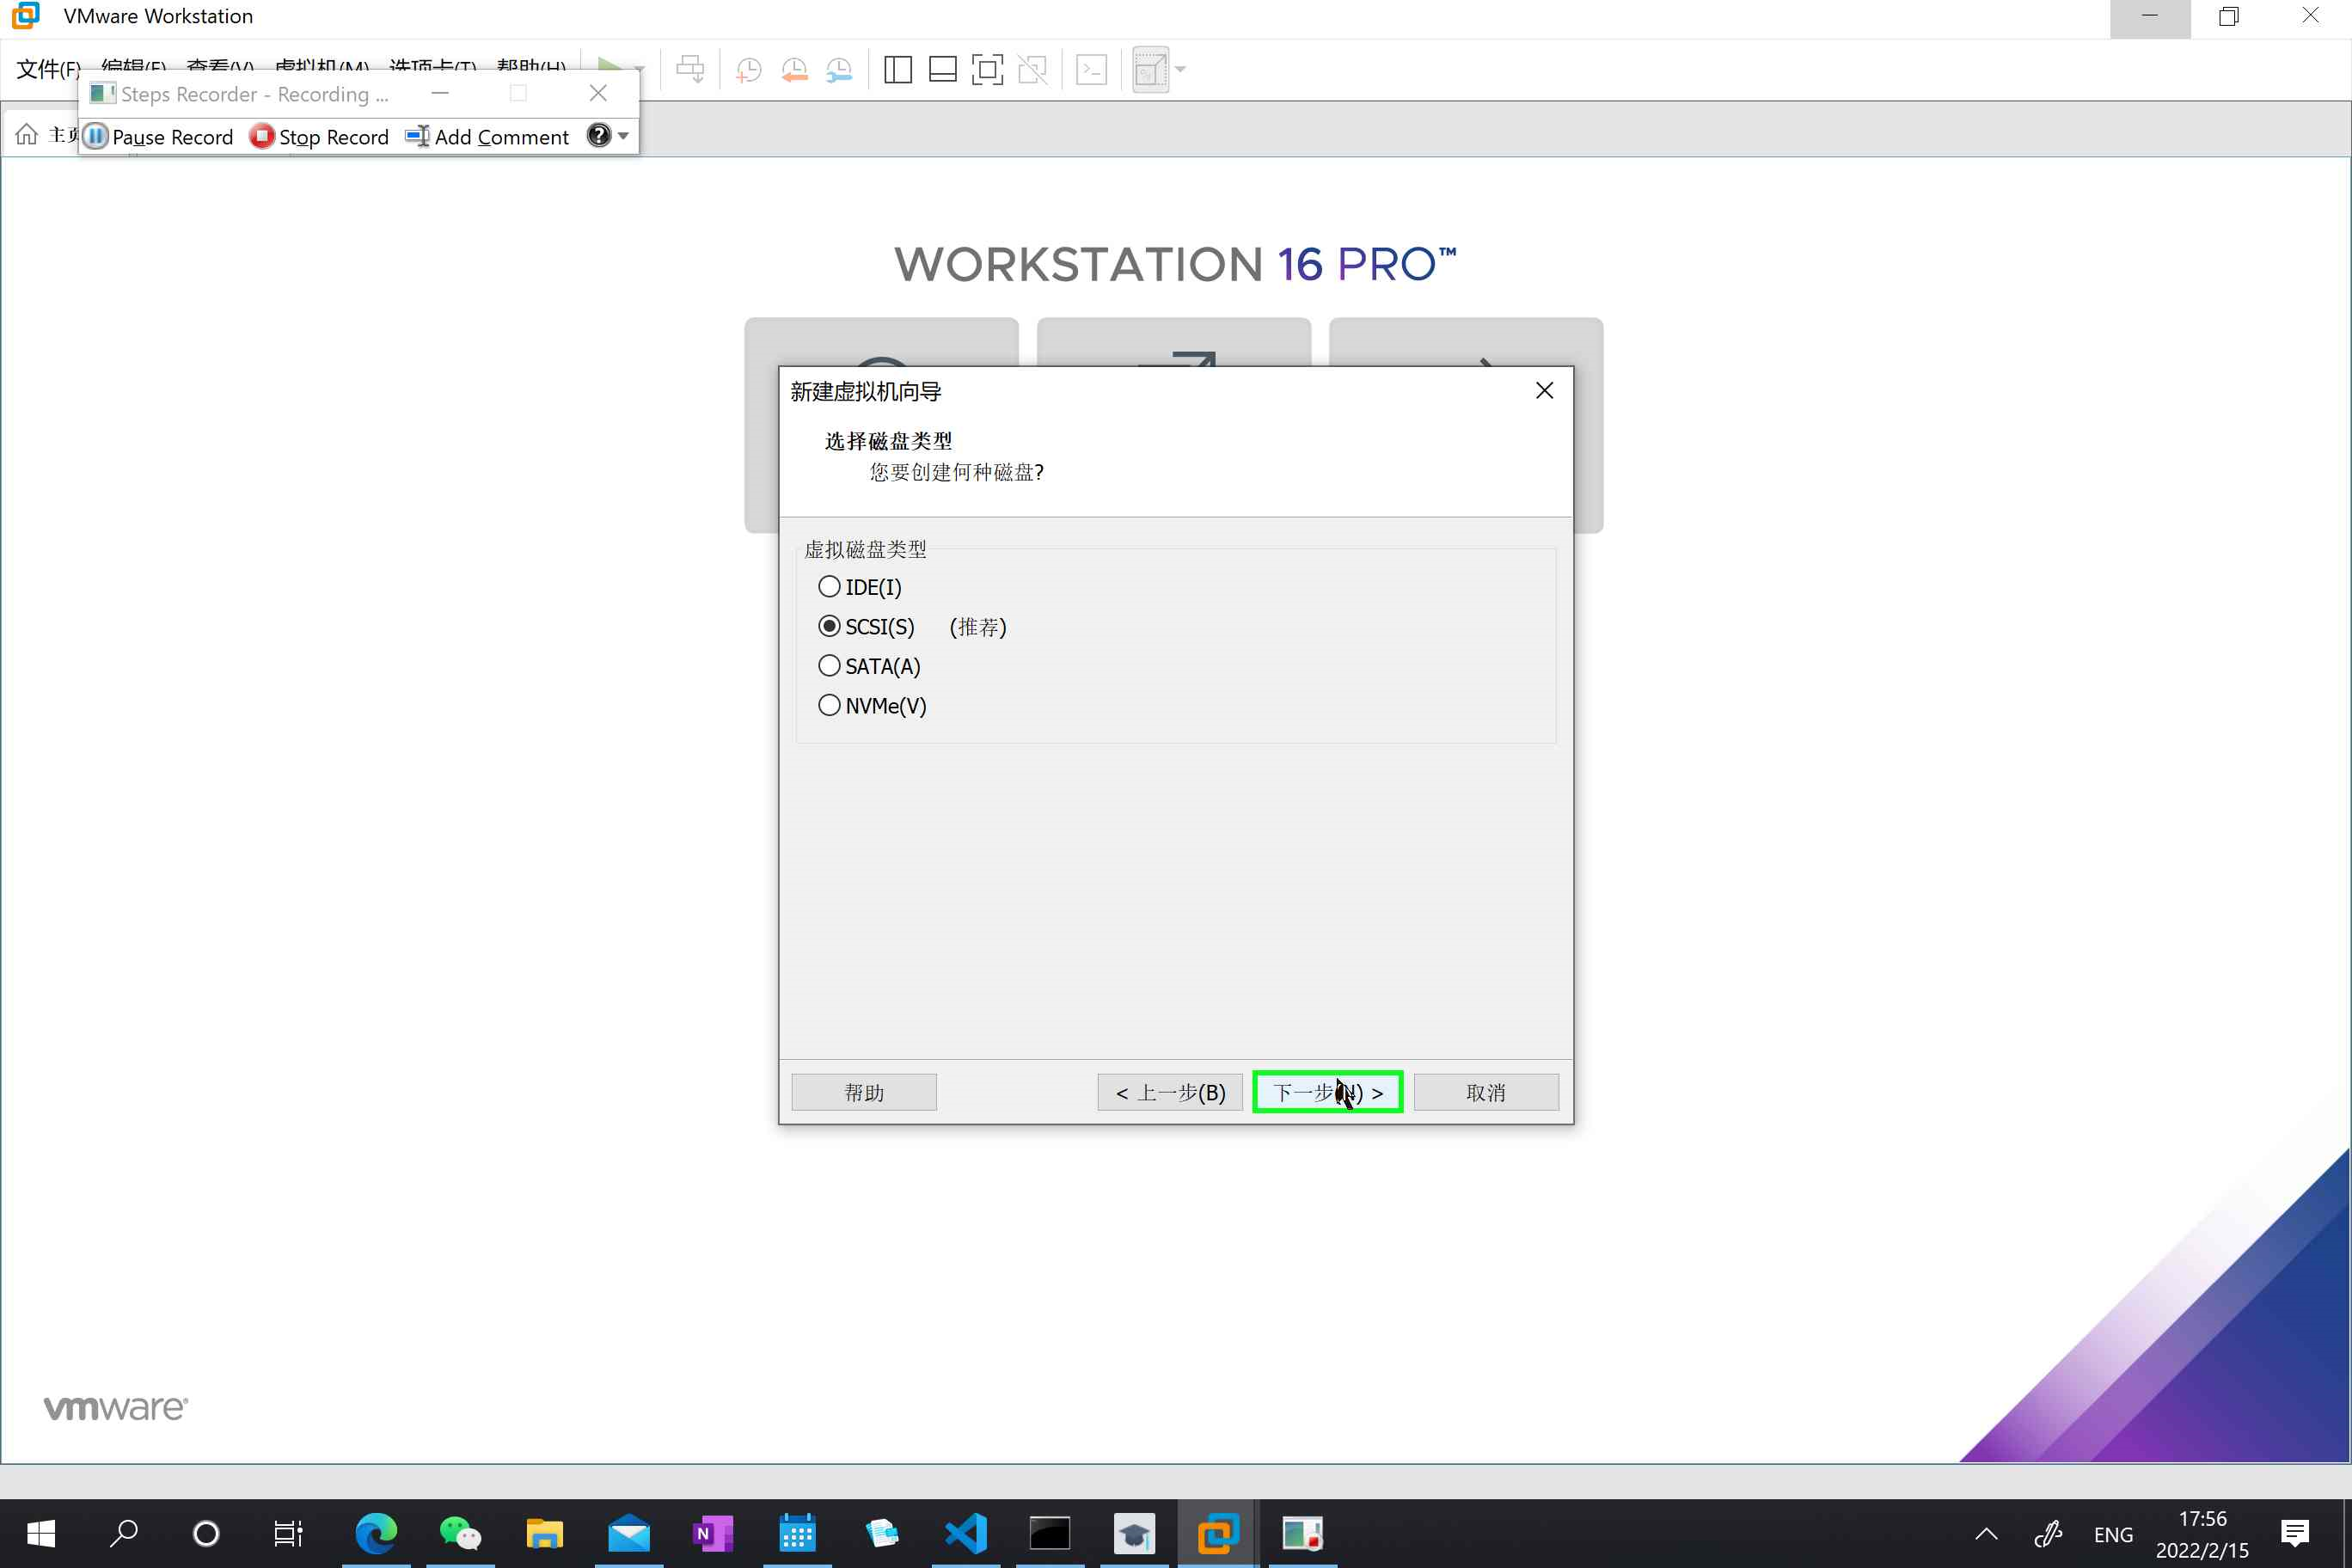
\includegraphics[width=0.8\textwidth]{assets/u14.png}
    \end{figure}
    \begin{figure}[H]
        \centering
        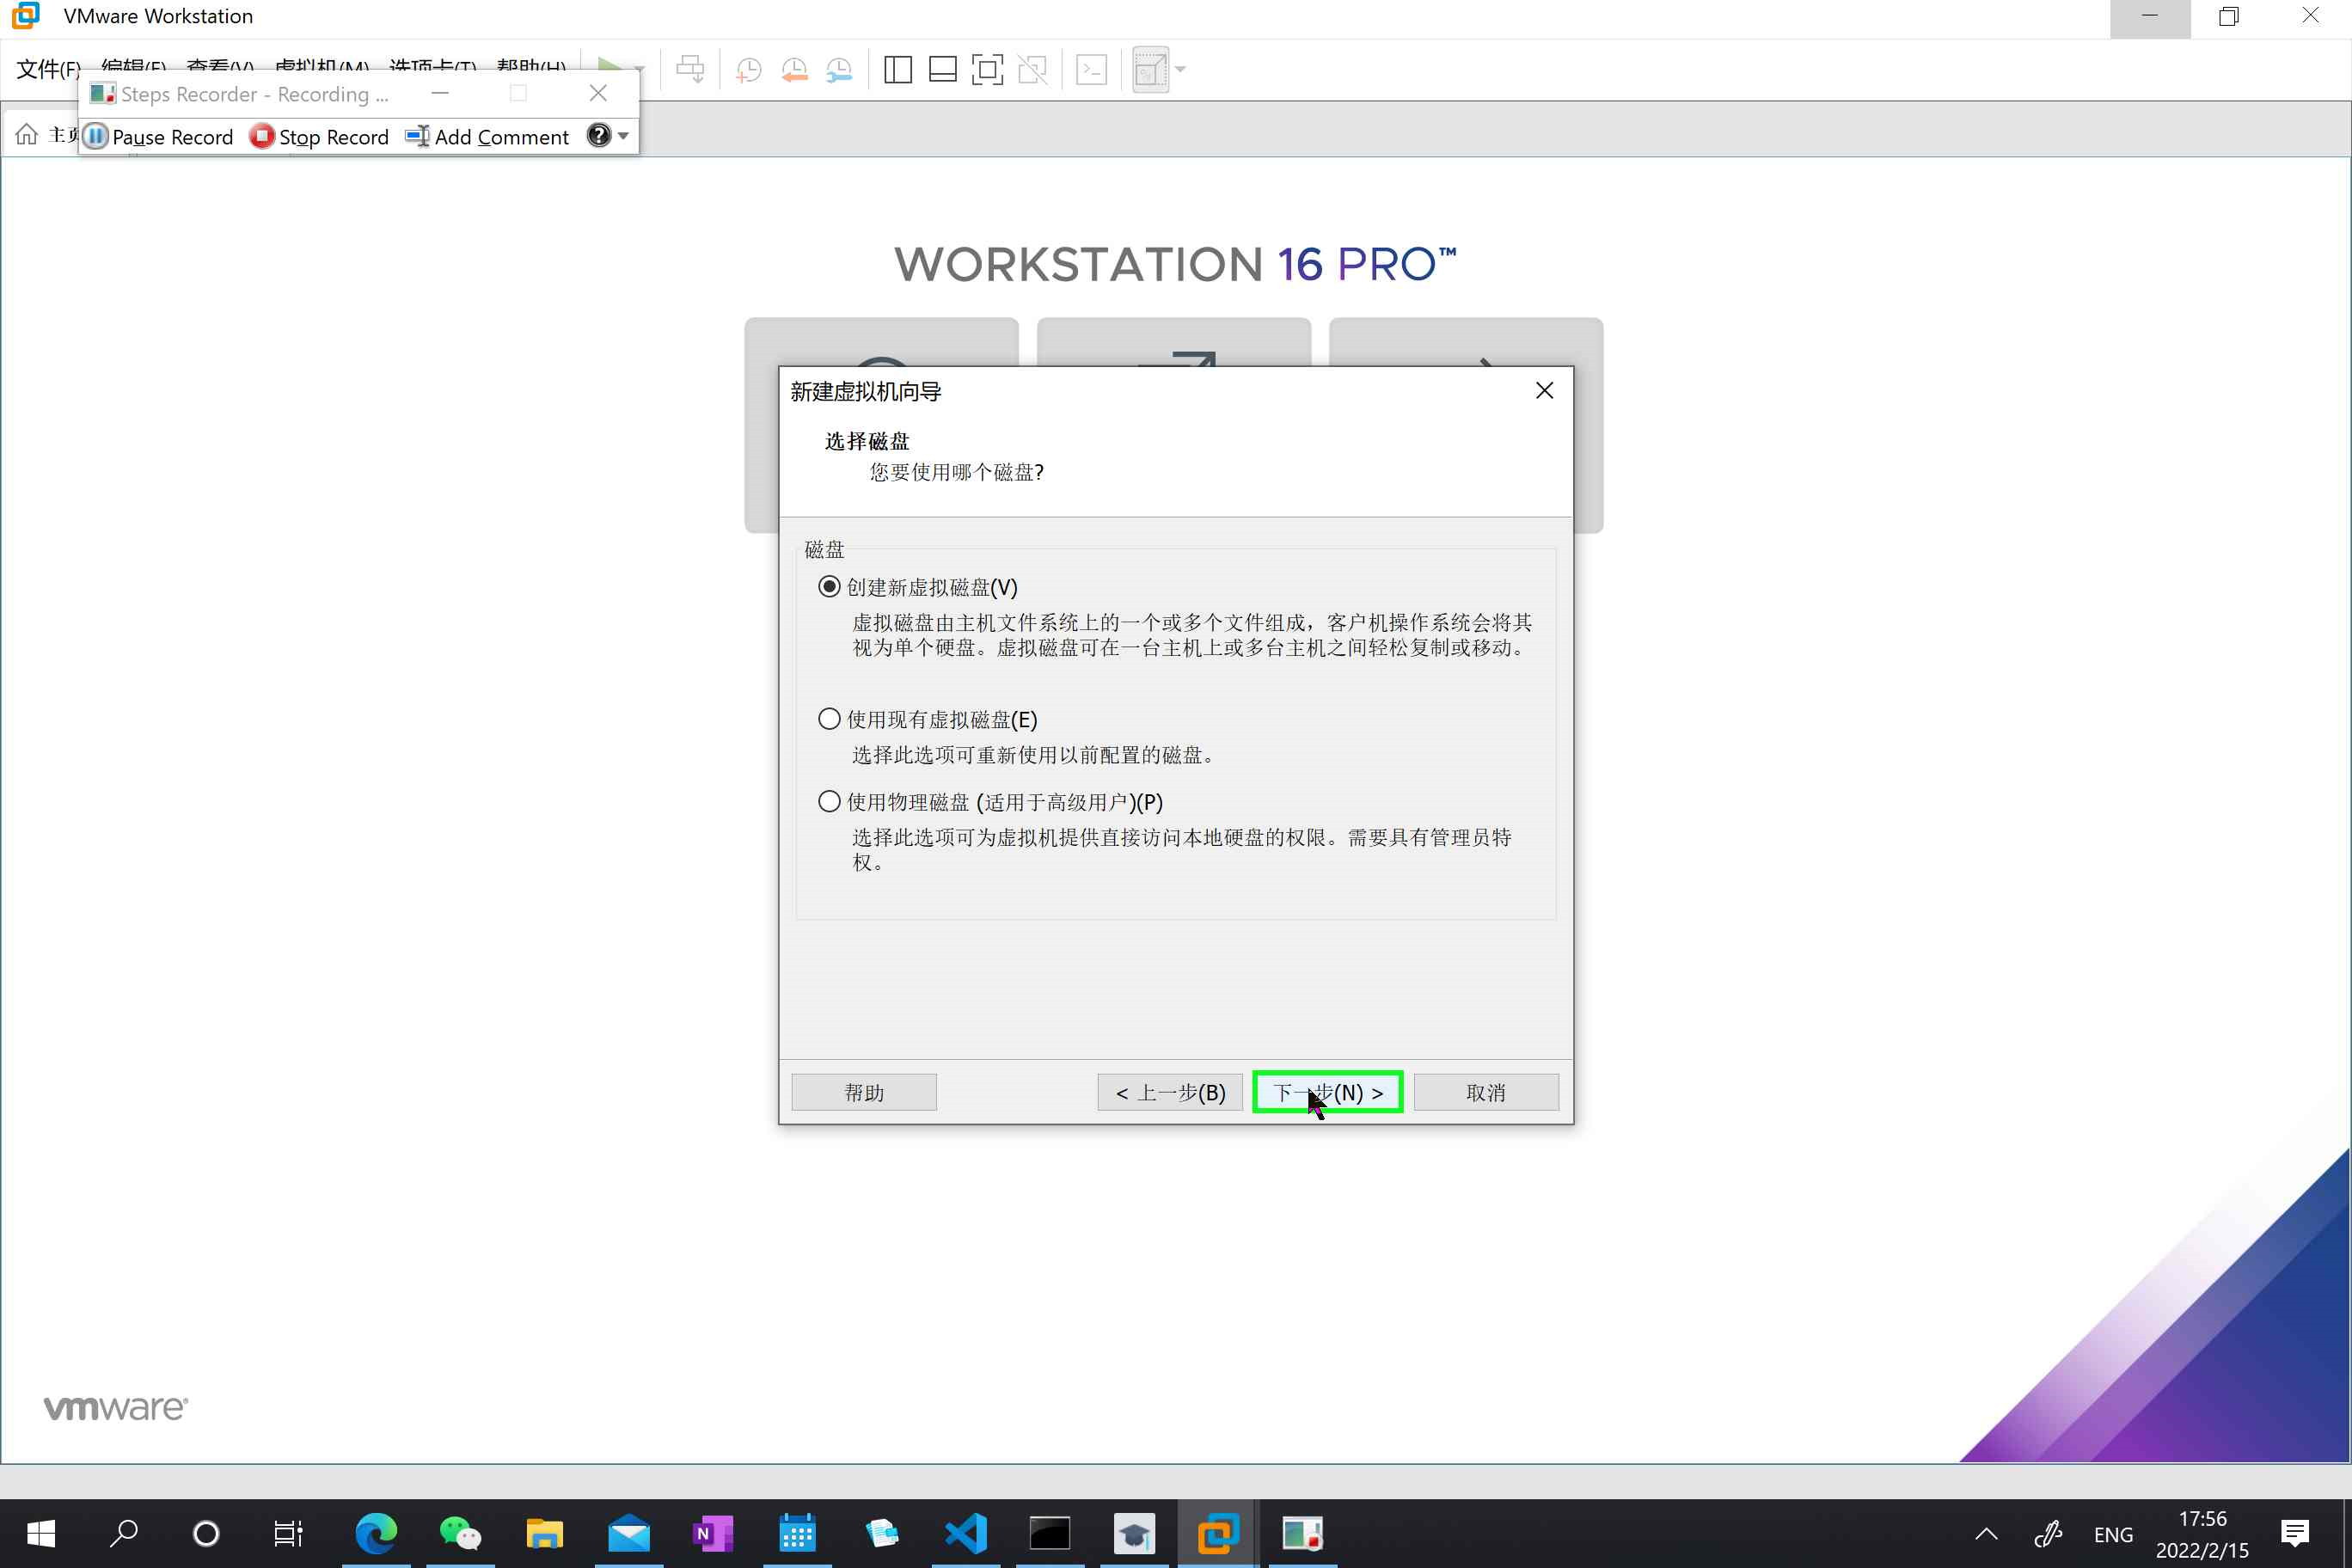
\includegraphics[width=0.8\textwidth]{assets/u15.png}
    \end{figure}
    \begin{figure}[H]
        \centering
        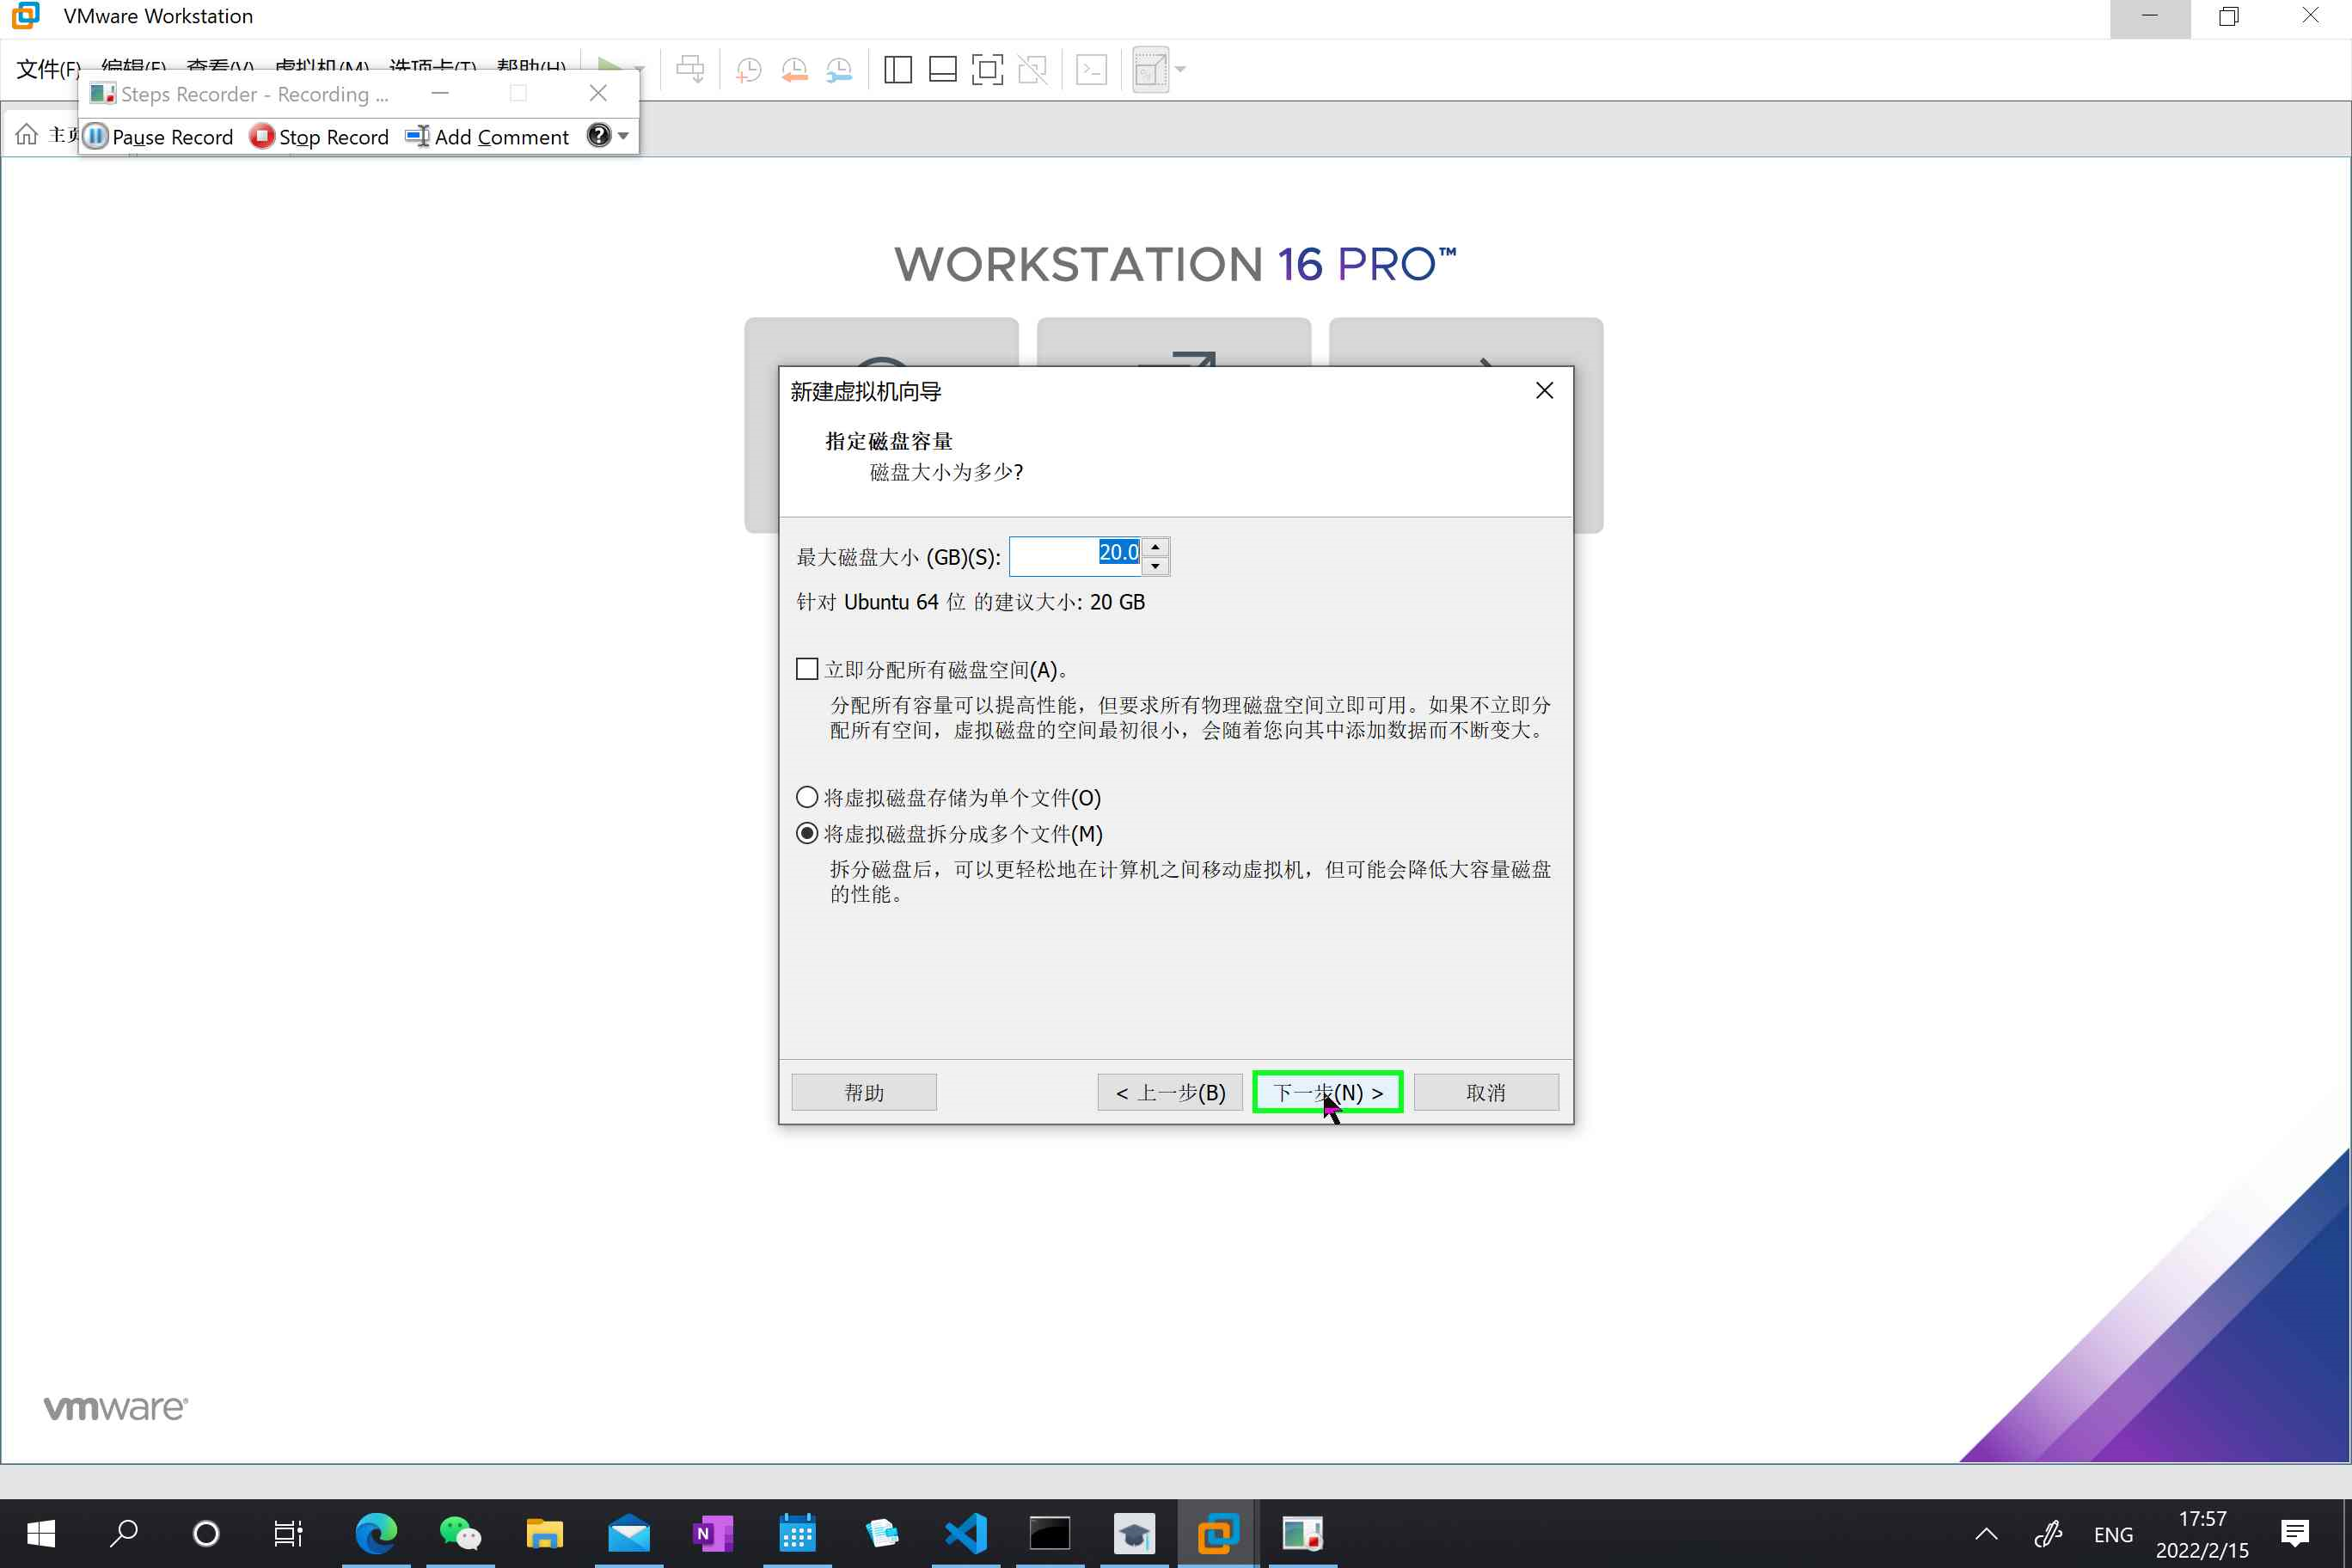
\includegraphics[width=0.8\textwidth]{assets/u16.png}
    \end{figure}
    \begin{figure}[H]
        \centering
        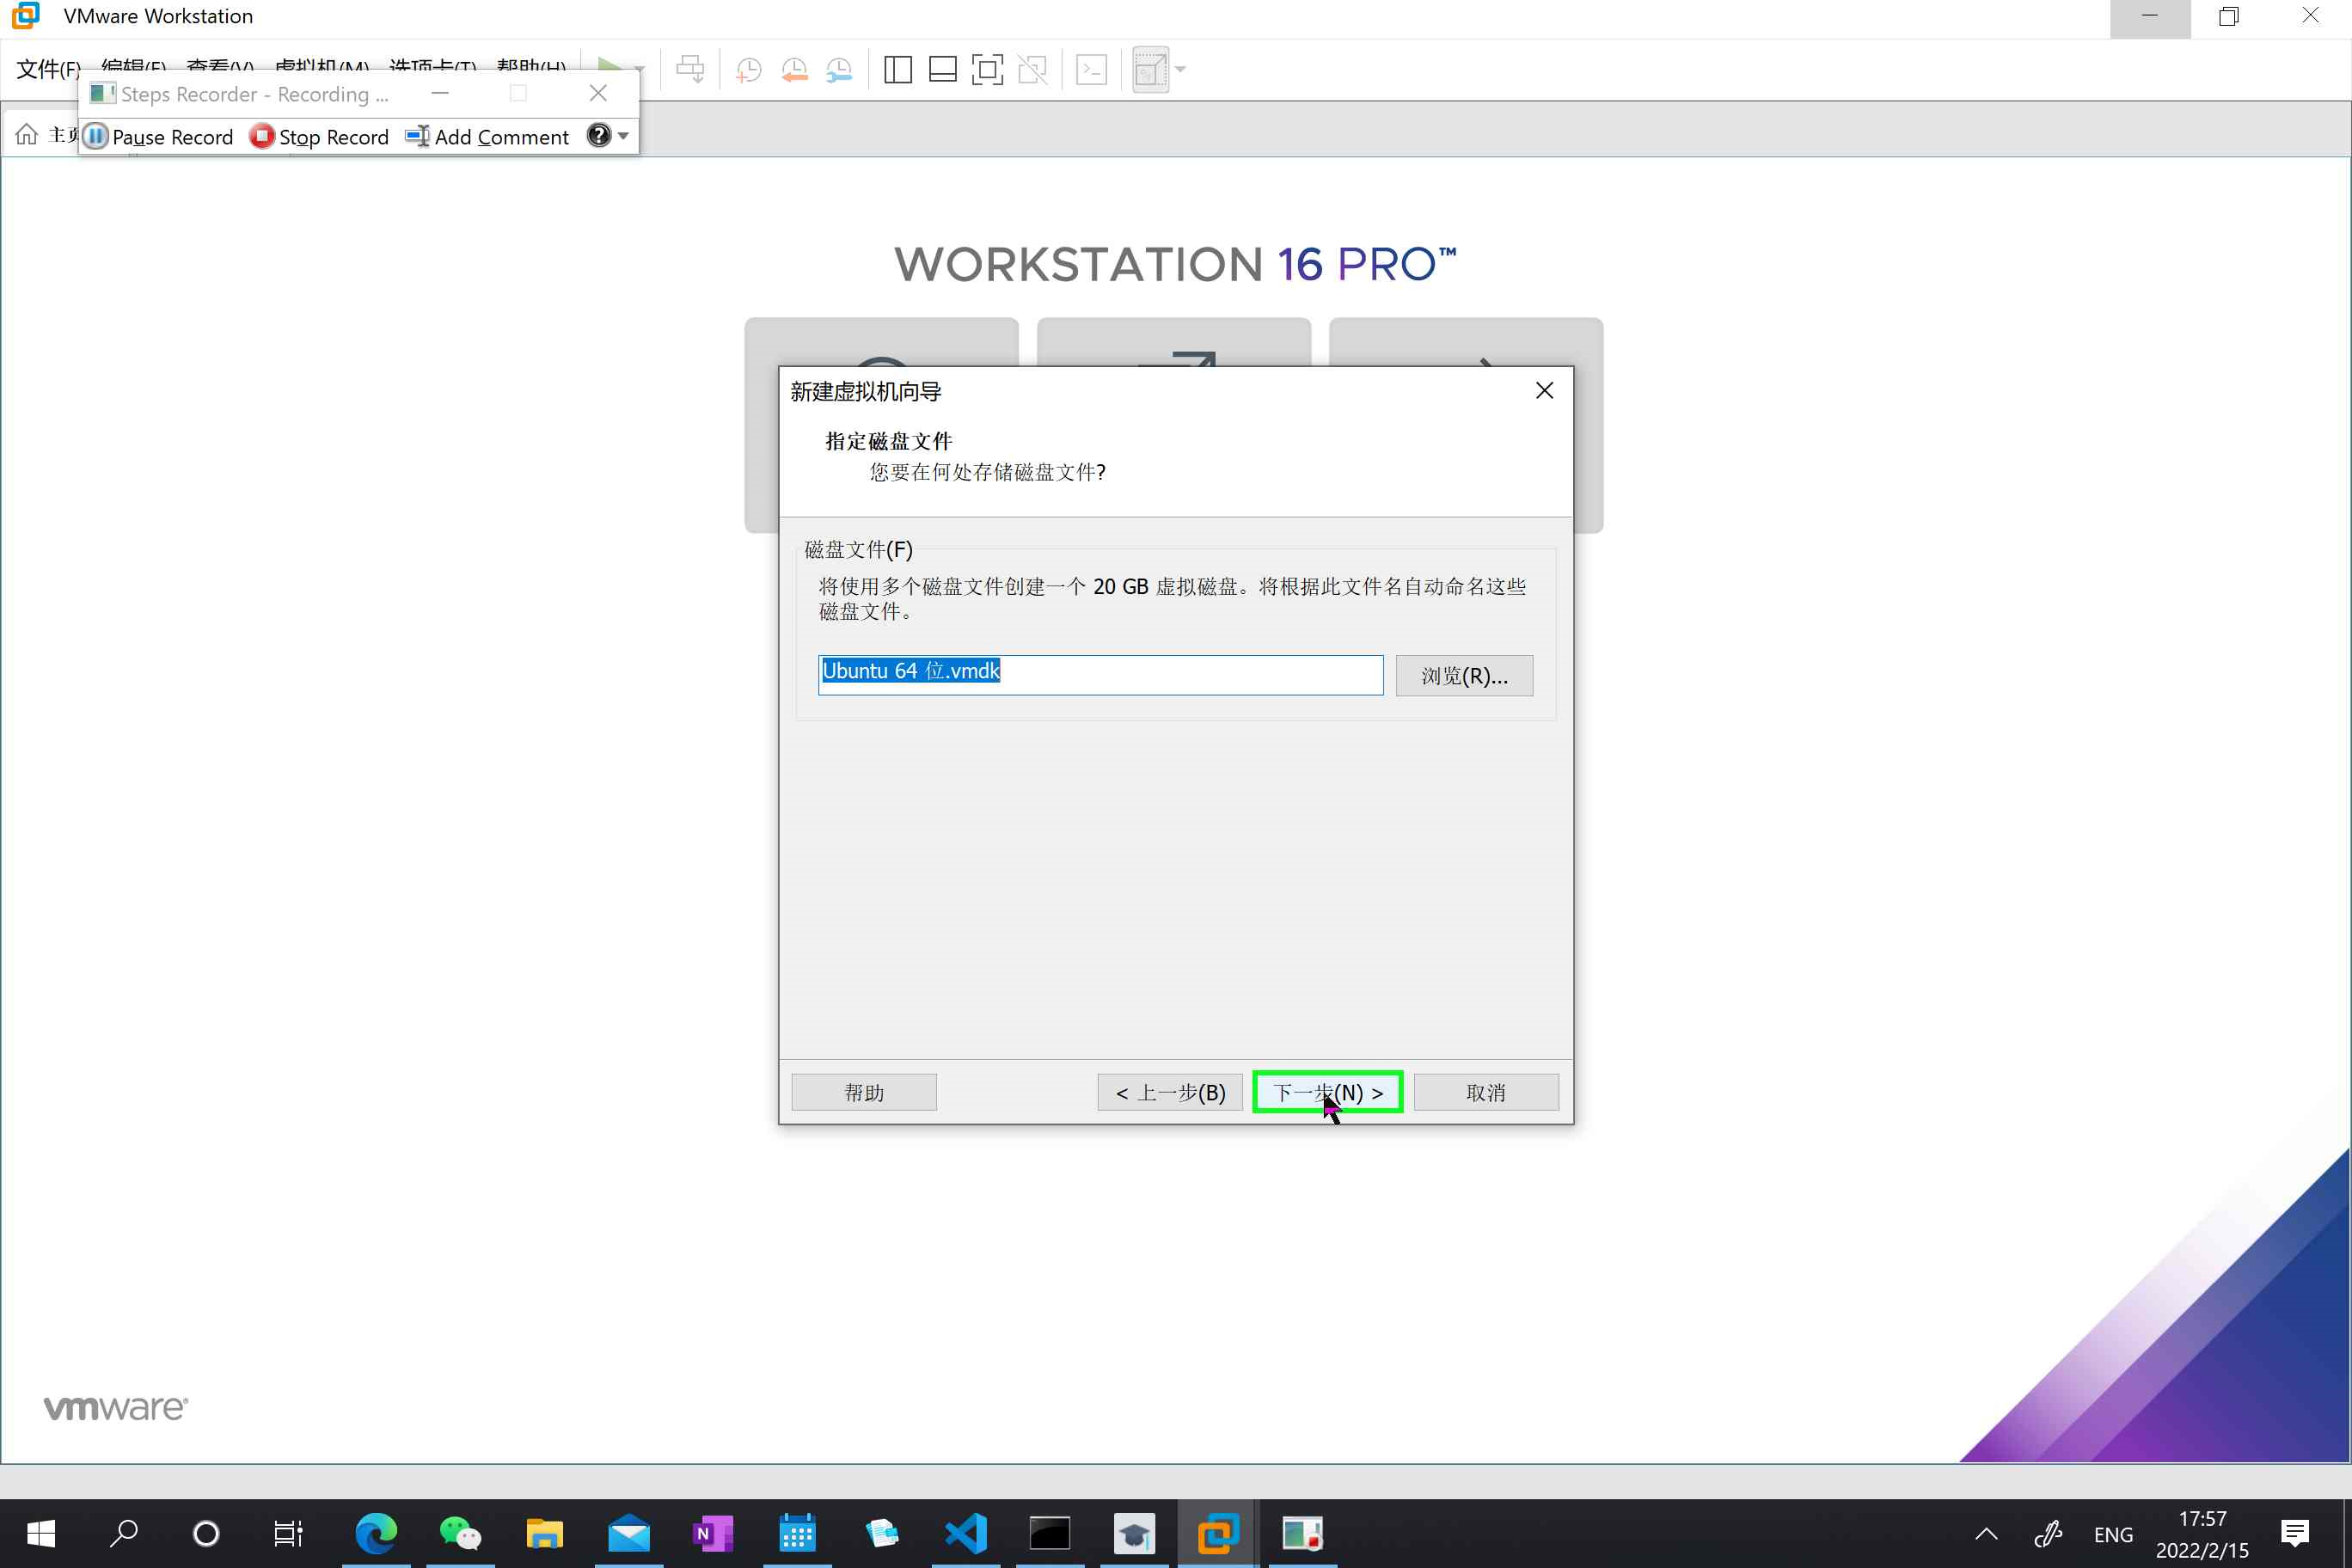
\includegraphics[width=0.8\textwidth]{assets/u17.png}
    \end{figure}
    \begin{figure}[H]
        \centering
        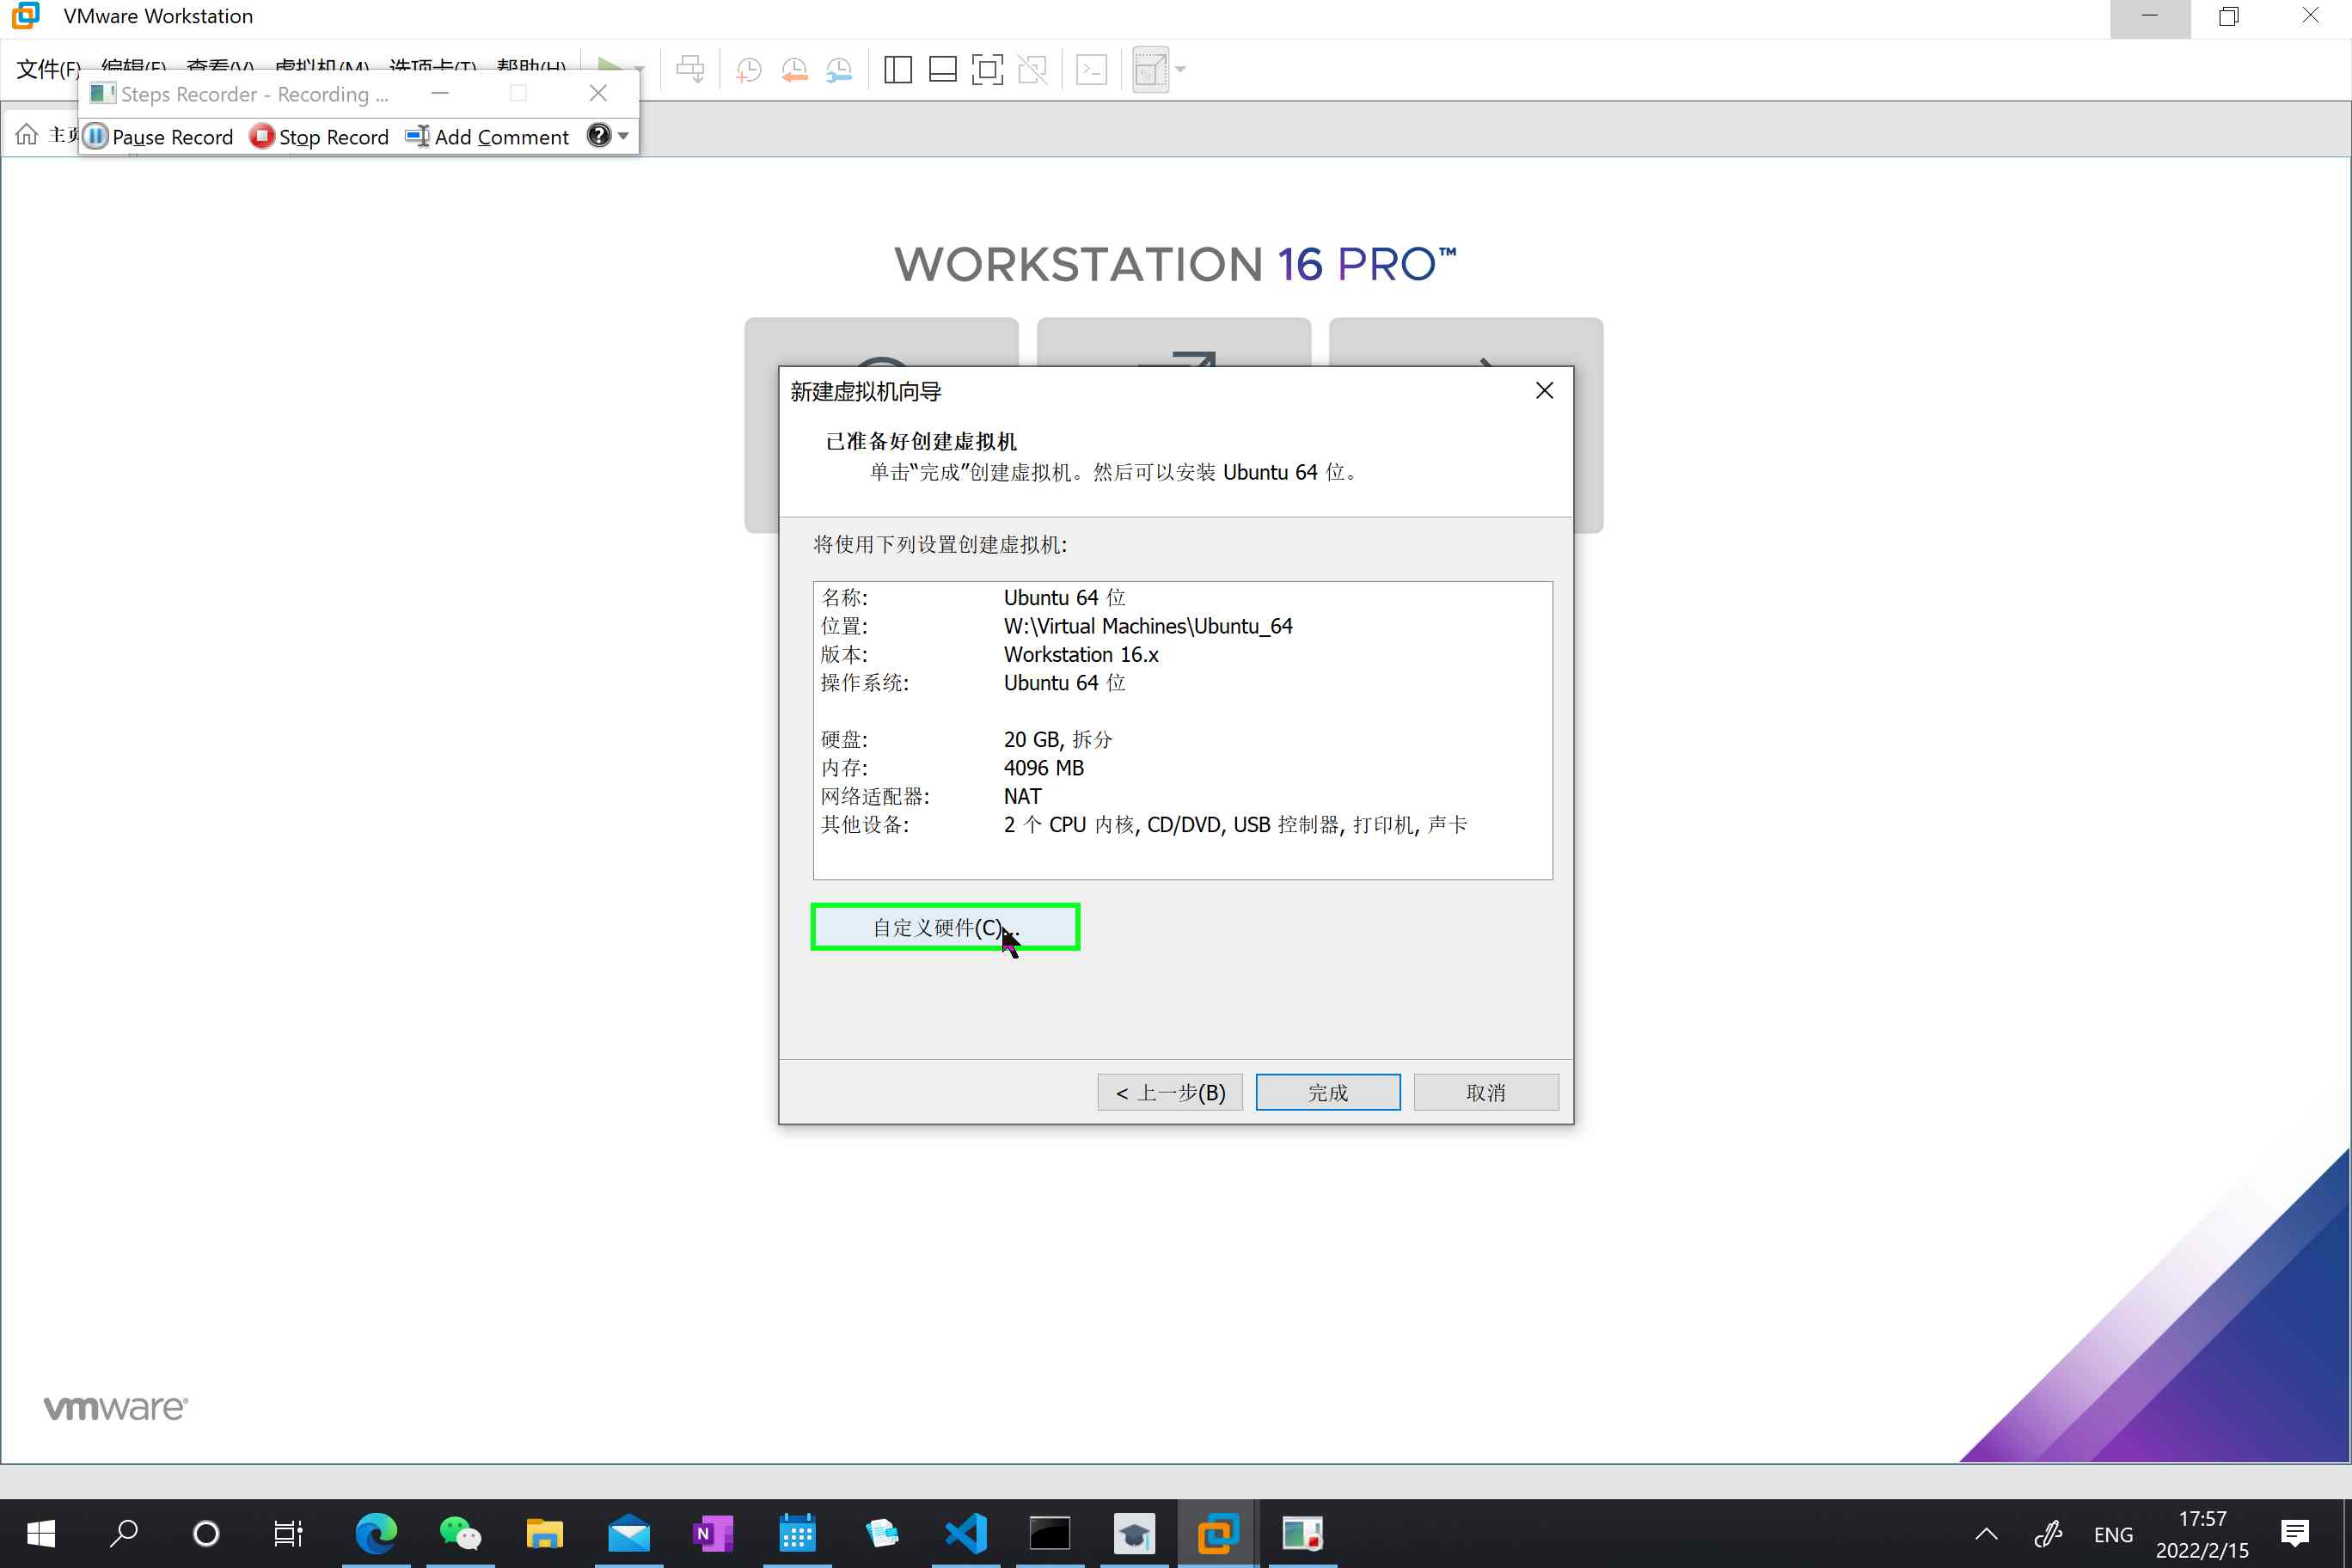
\includegraphics[width=0.8\textwidth]{assets/u18.png}
    \end{figure}
    \begin{figure}[H]
        \centering
        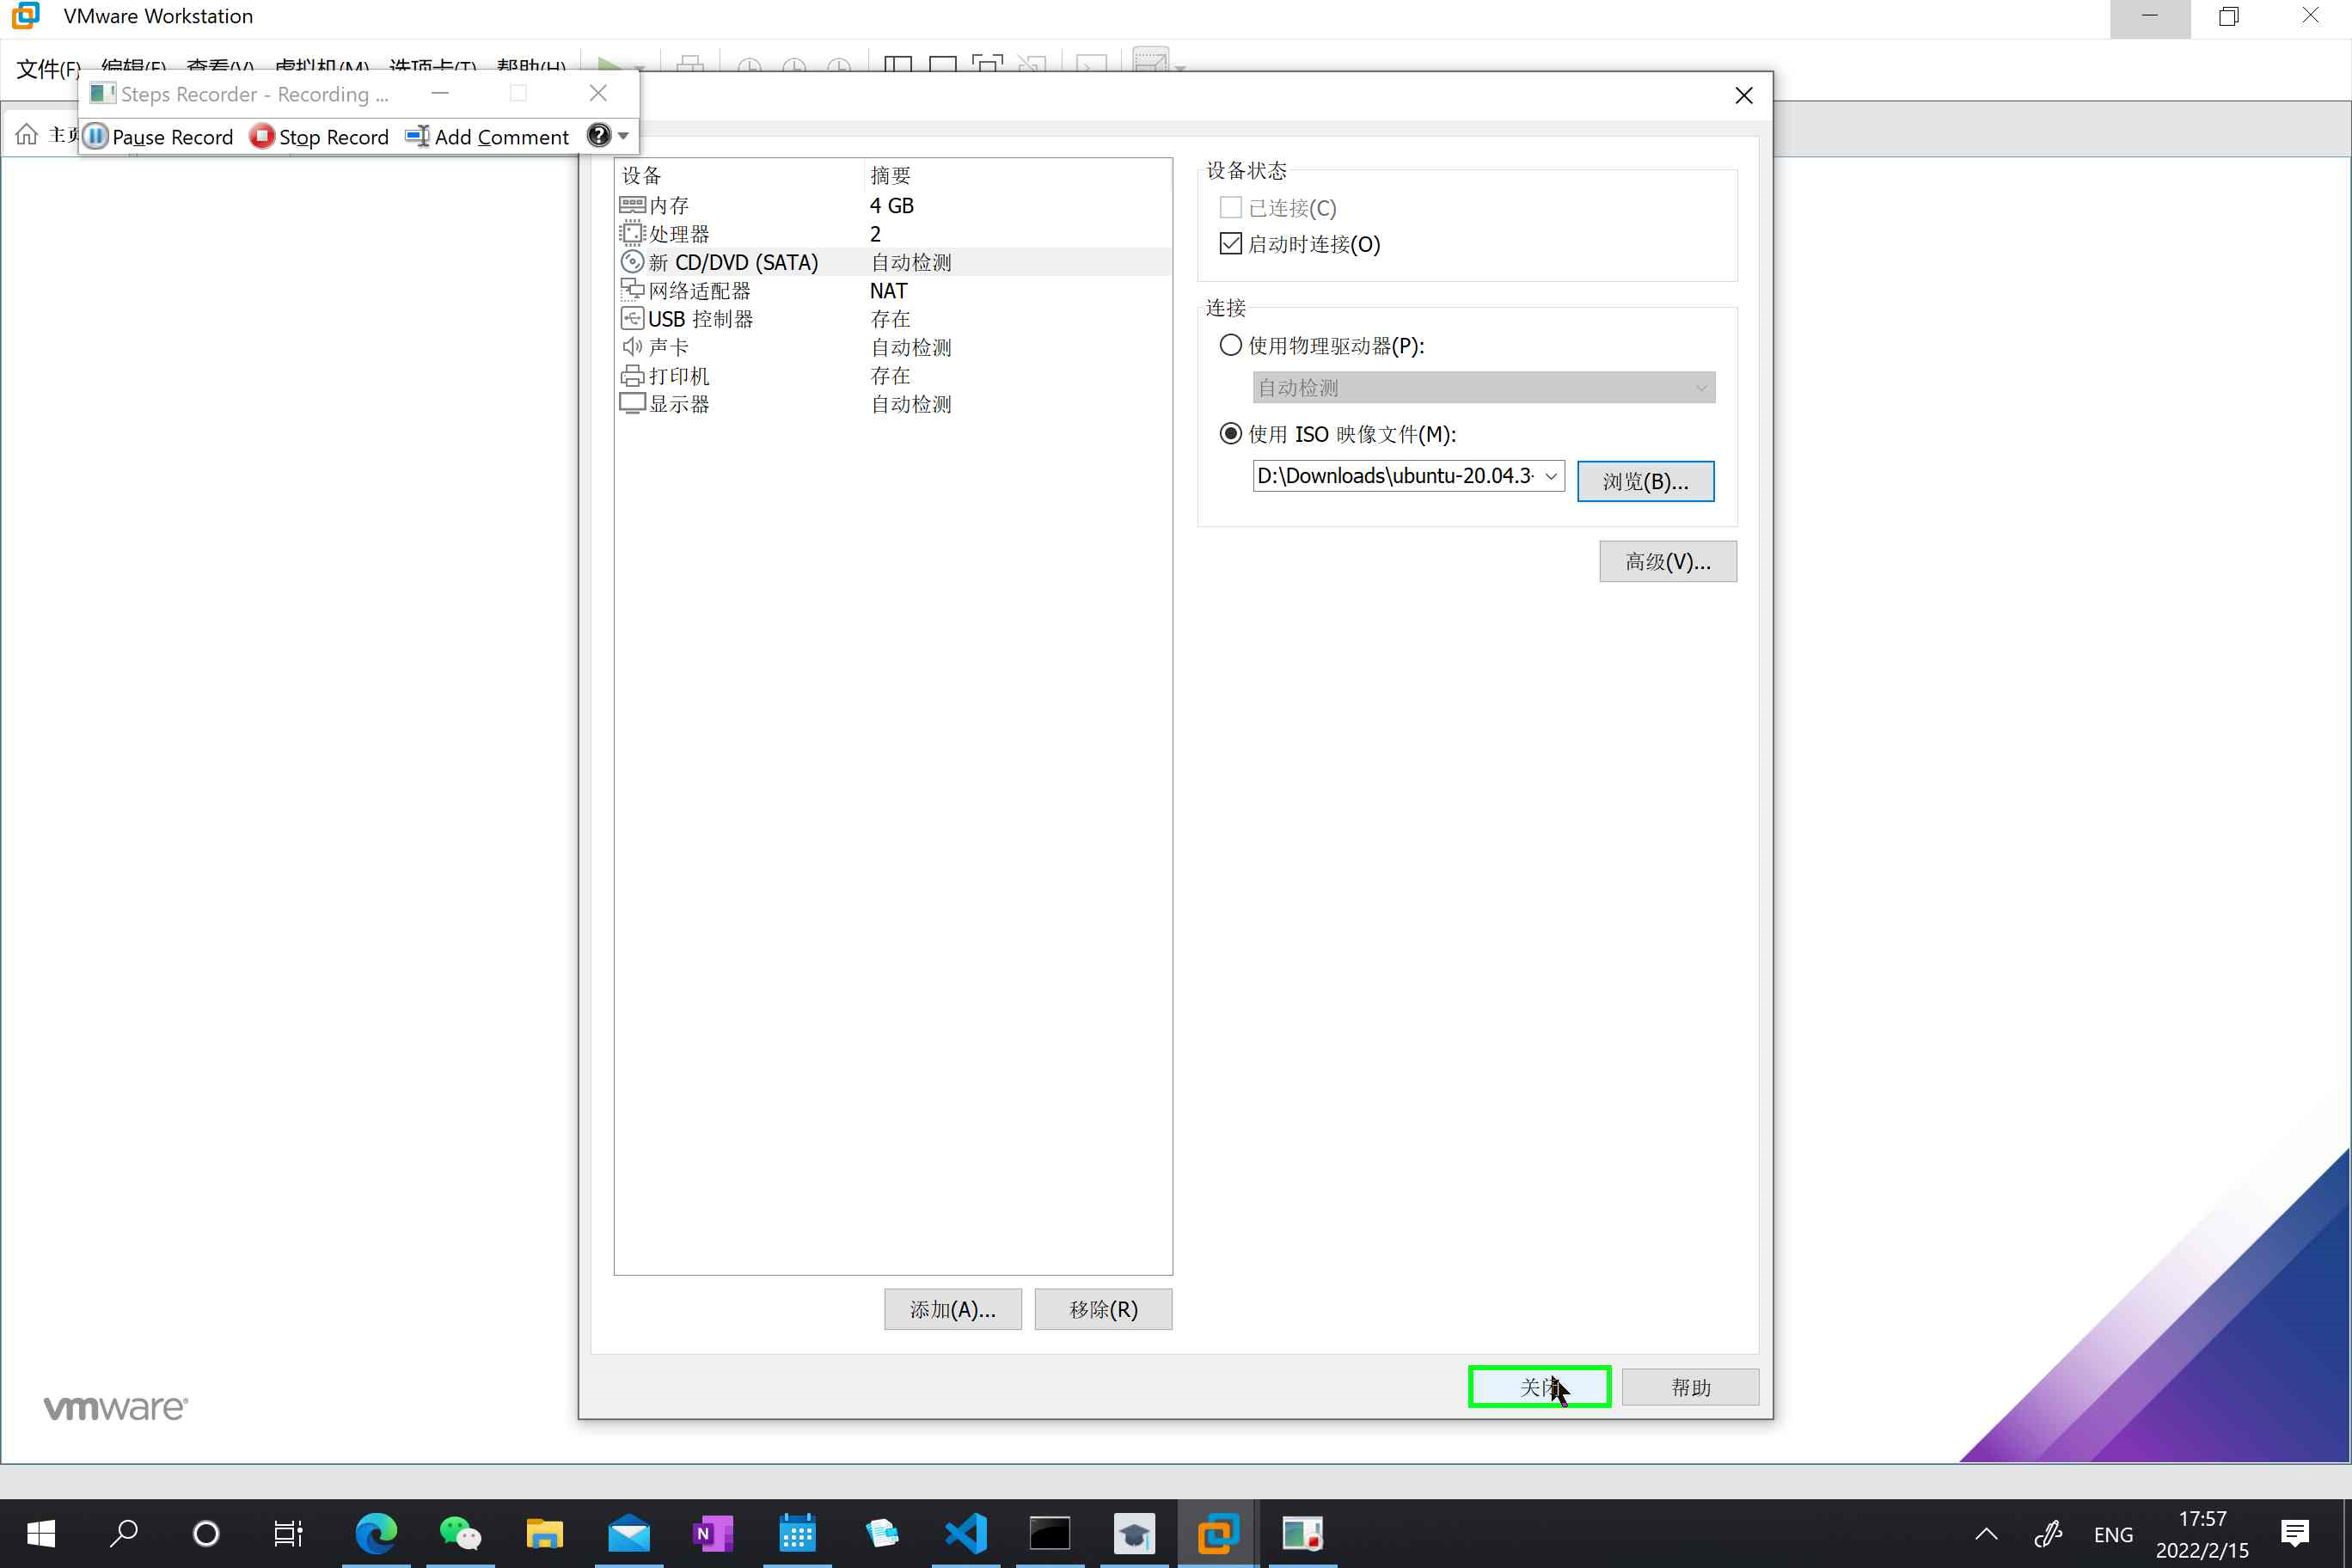
\includegraphics[width=0.8\textwidth]{assets/u19.png}
    \end{figure}
    \begin{figure}[H]
        \centering
        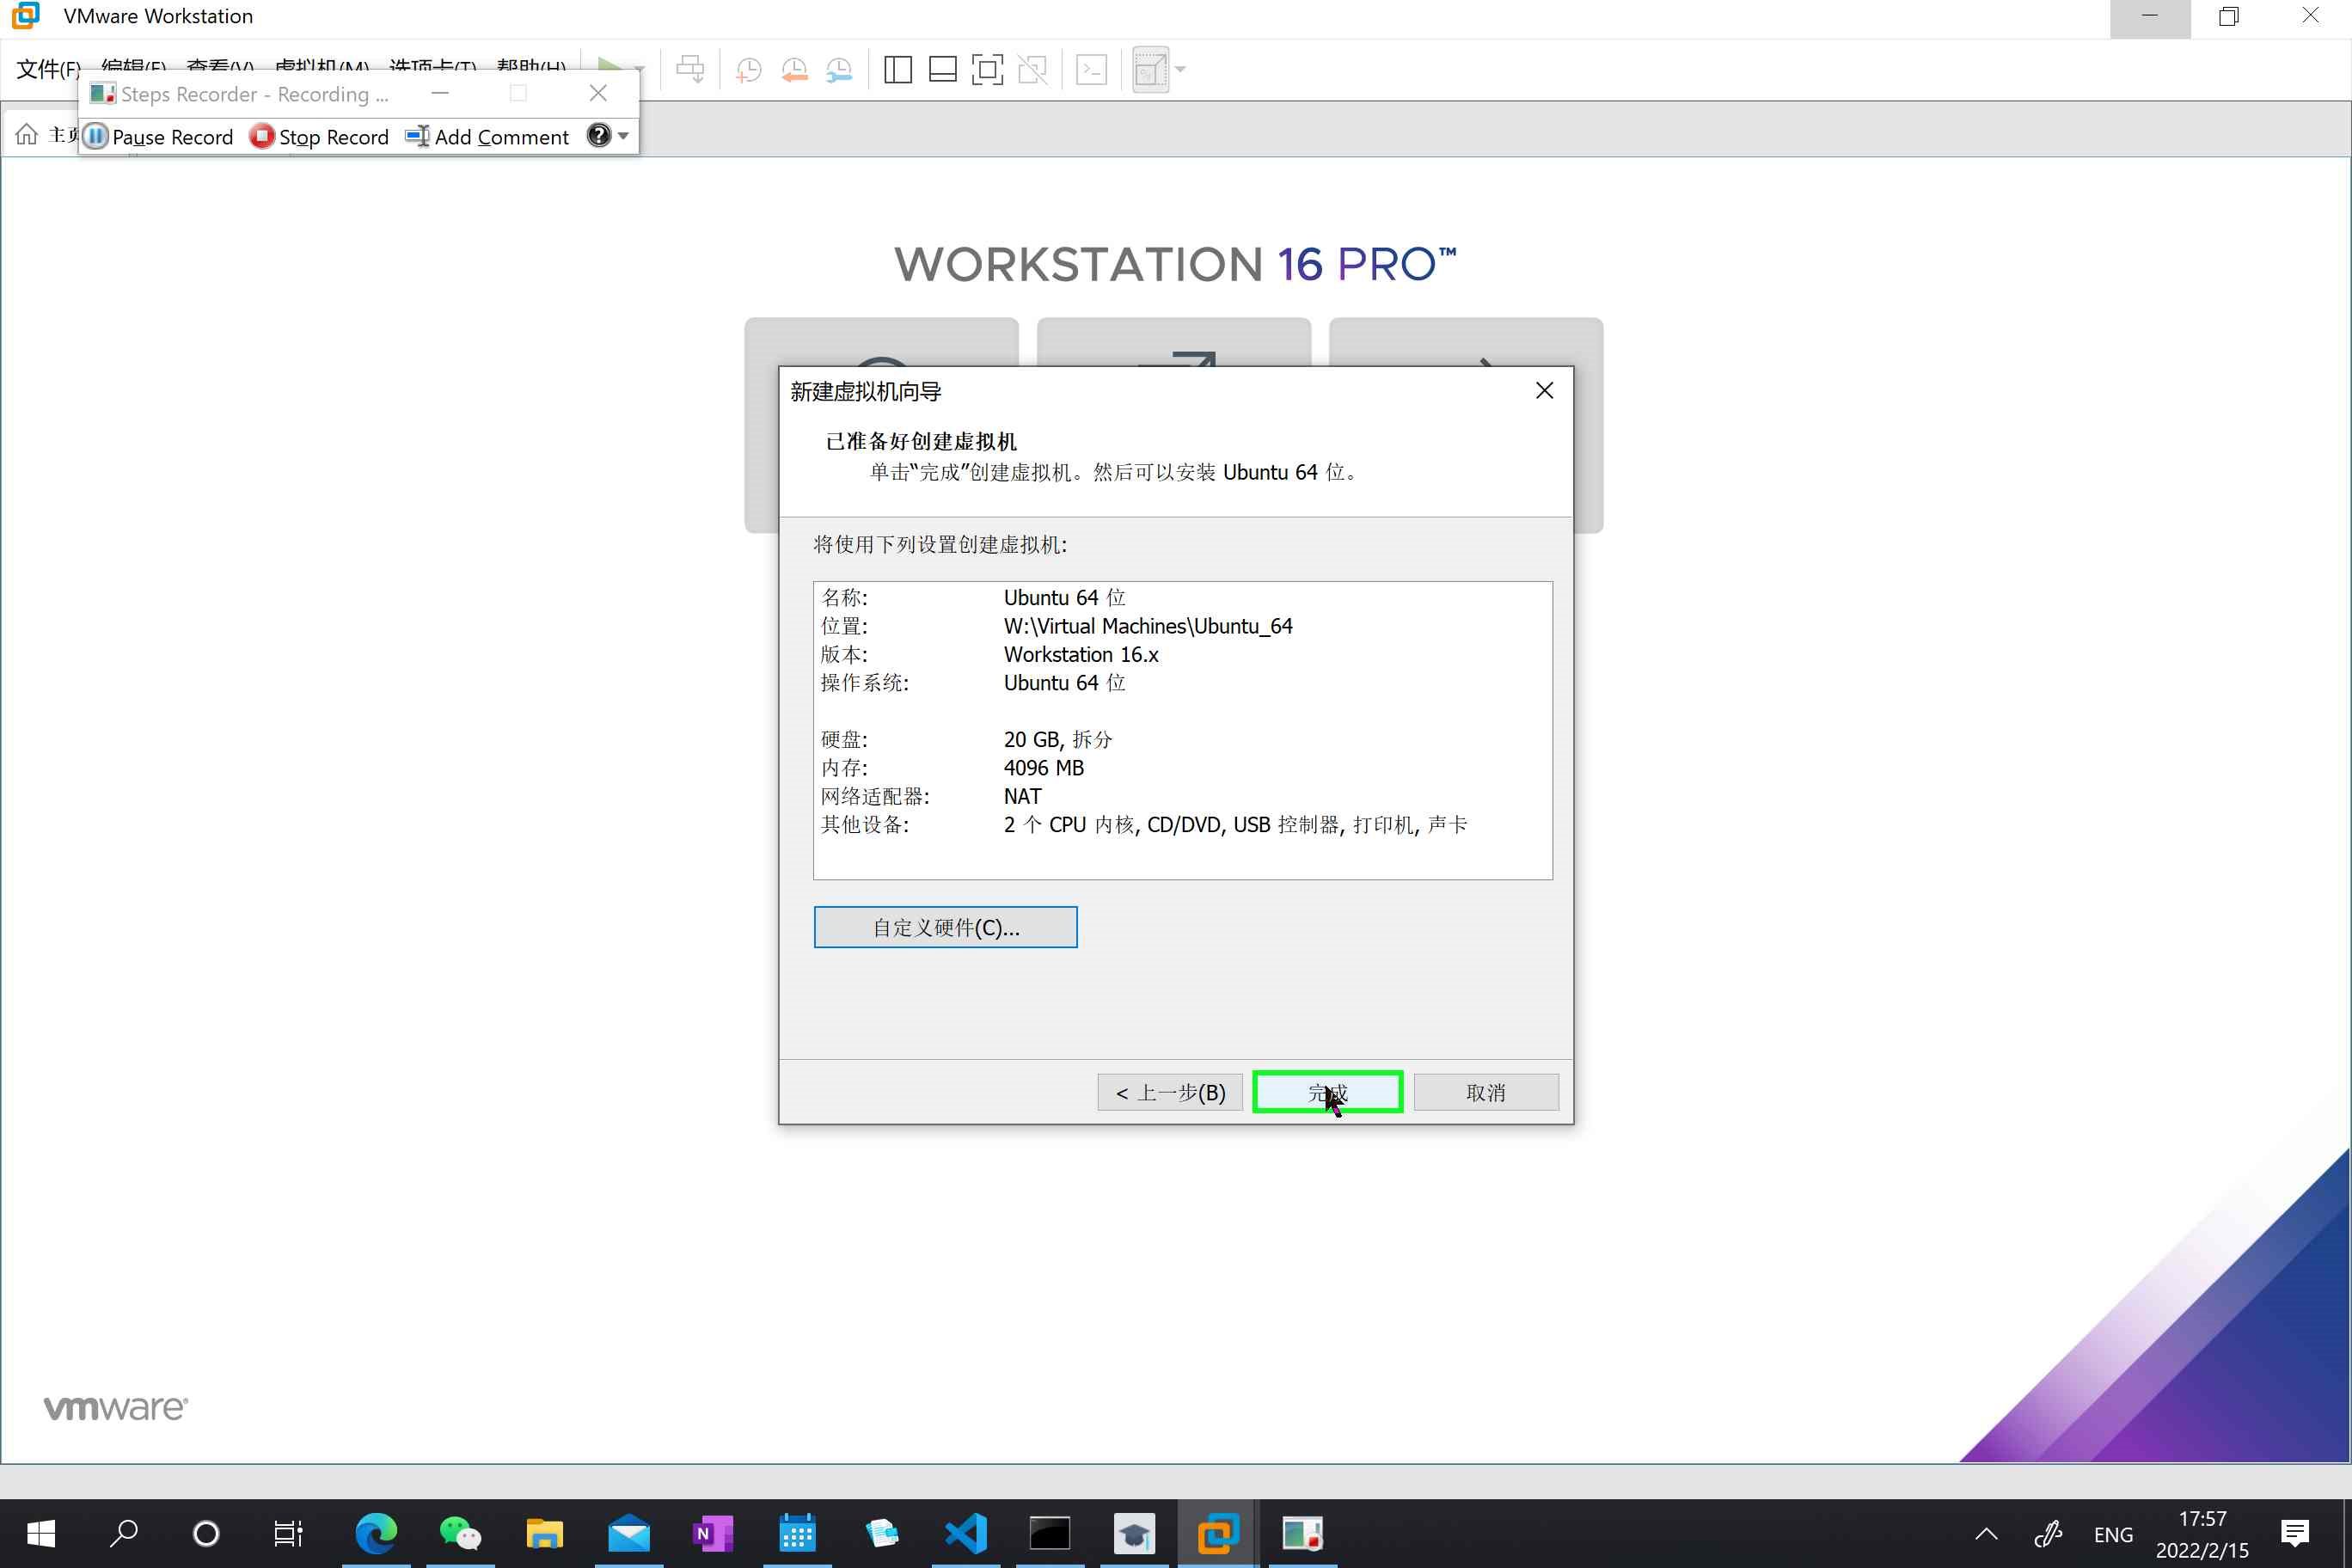
\includegraphics[width=0.8\textwidth]{assets/u20.png}
    \end{figure}
    

    \section{配置Ubuntu}
    在VMware中点击“启动虚拟机后,按照提示一路进行设置即可。”
    \begin{figure}[H]
        \centering
        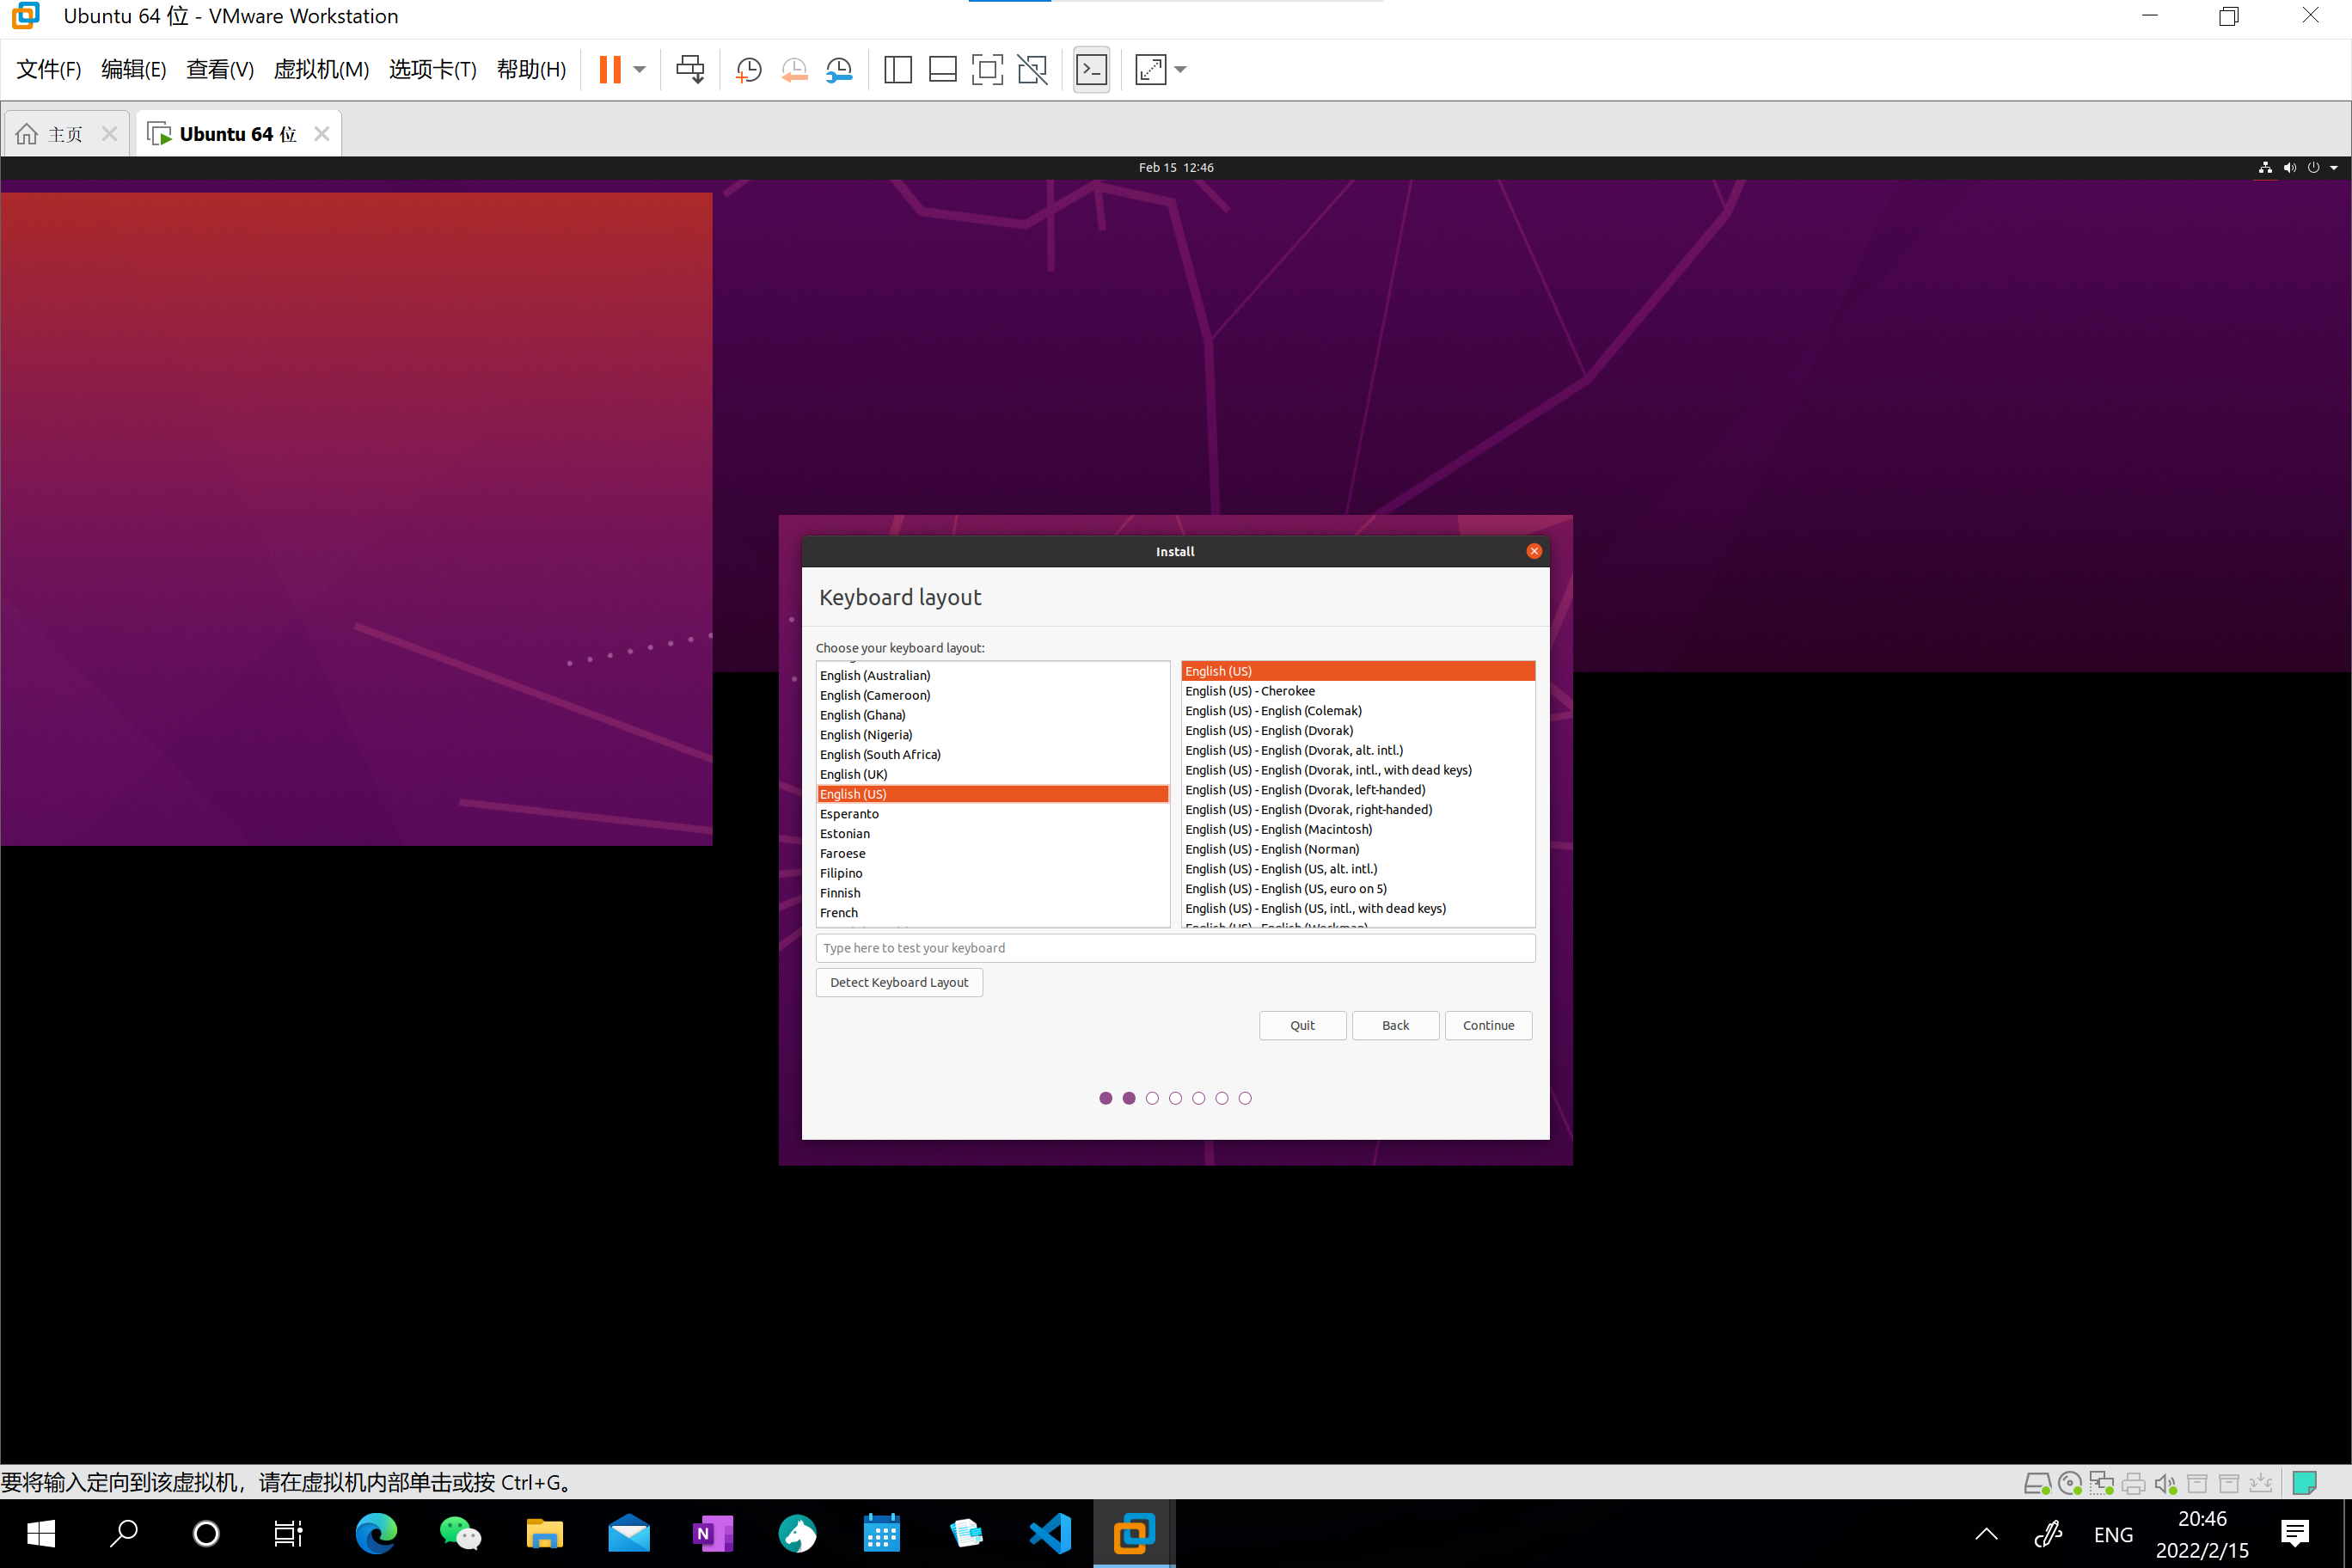
\includegraphics[width=0.8\textwidth]{assets/l1.png}
    \end{figure}
    \begin{figure}[H]
        \centering
        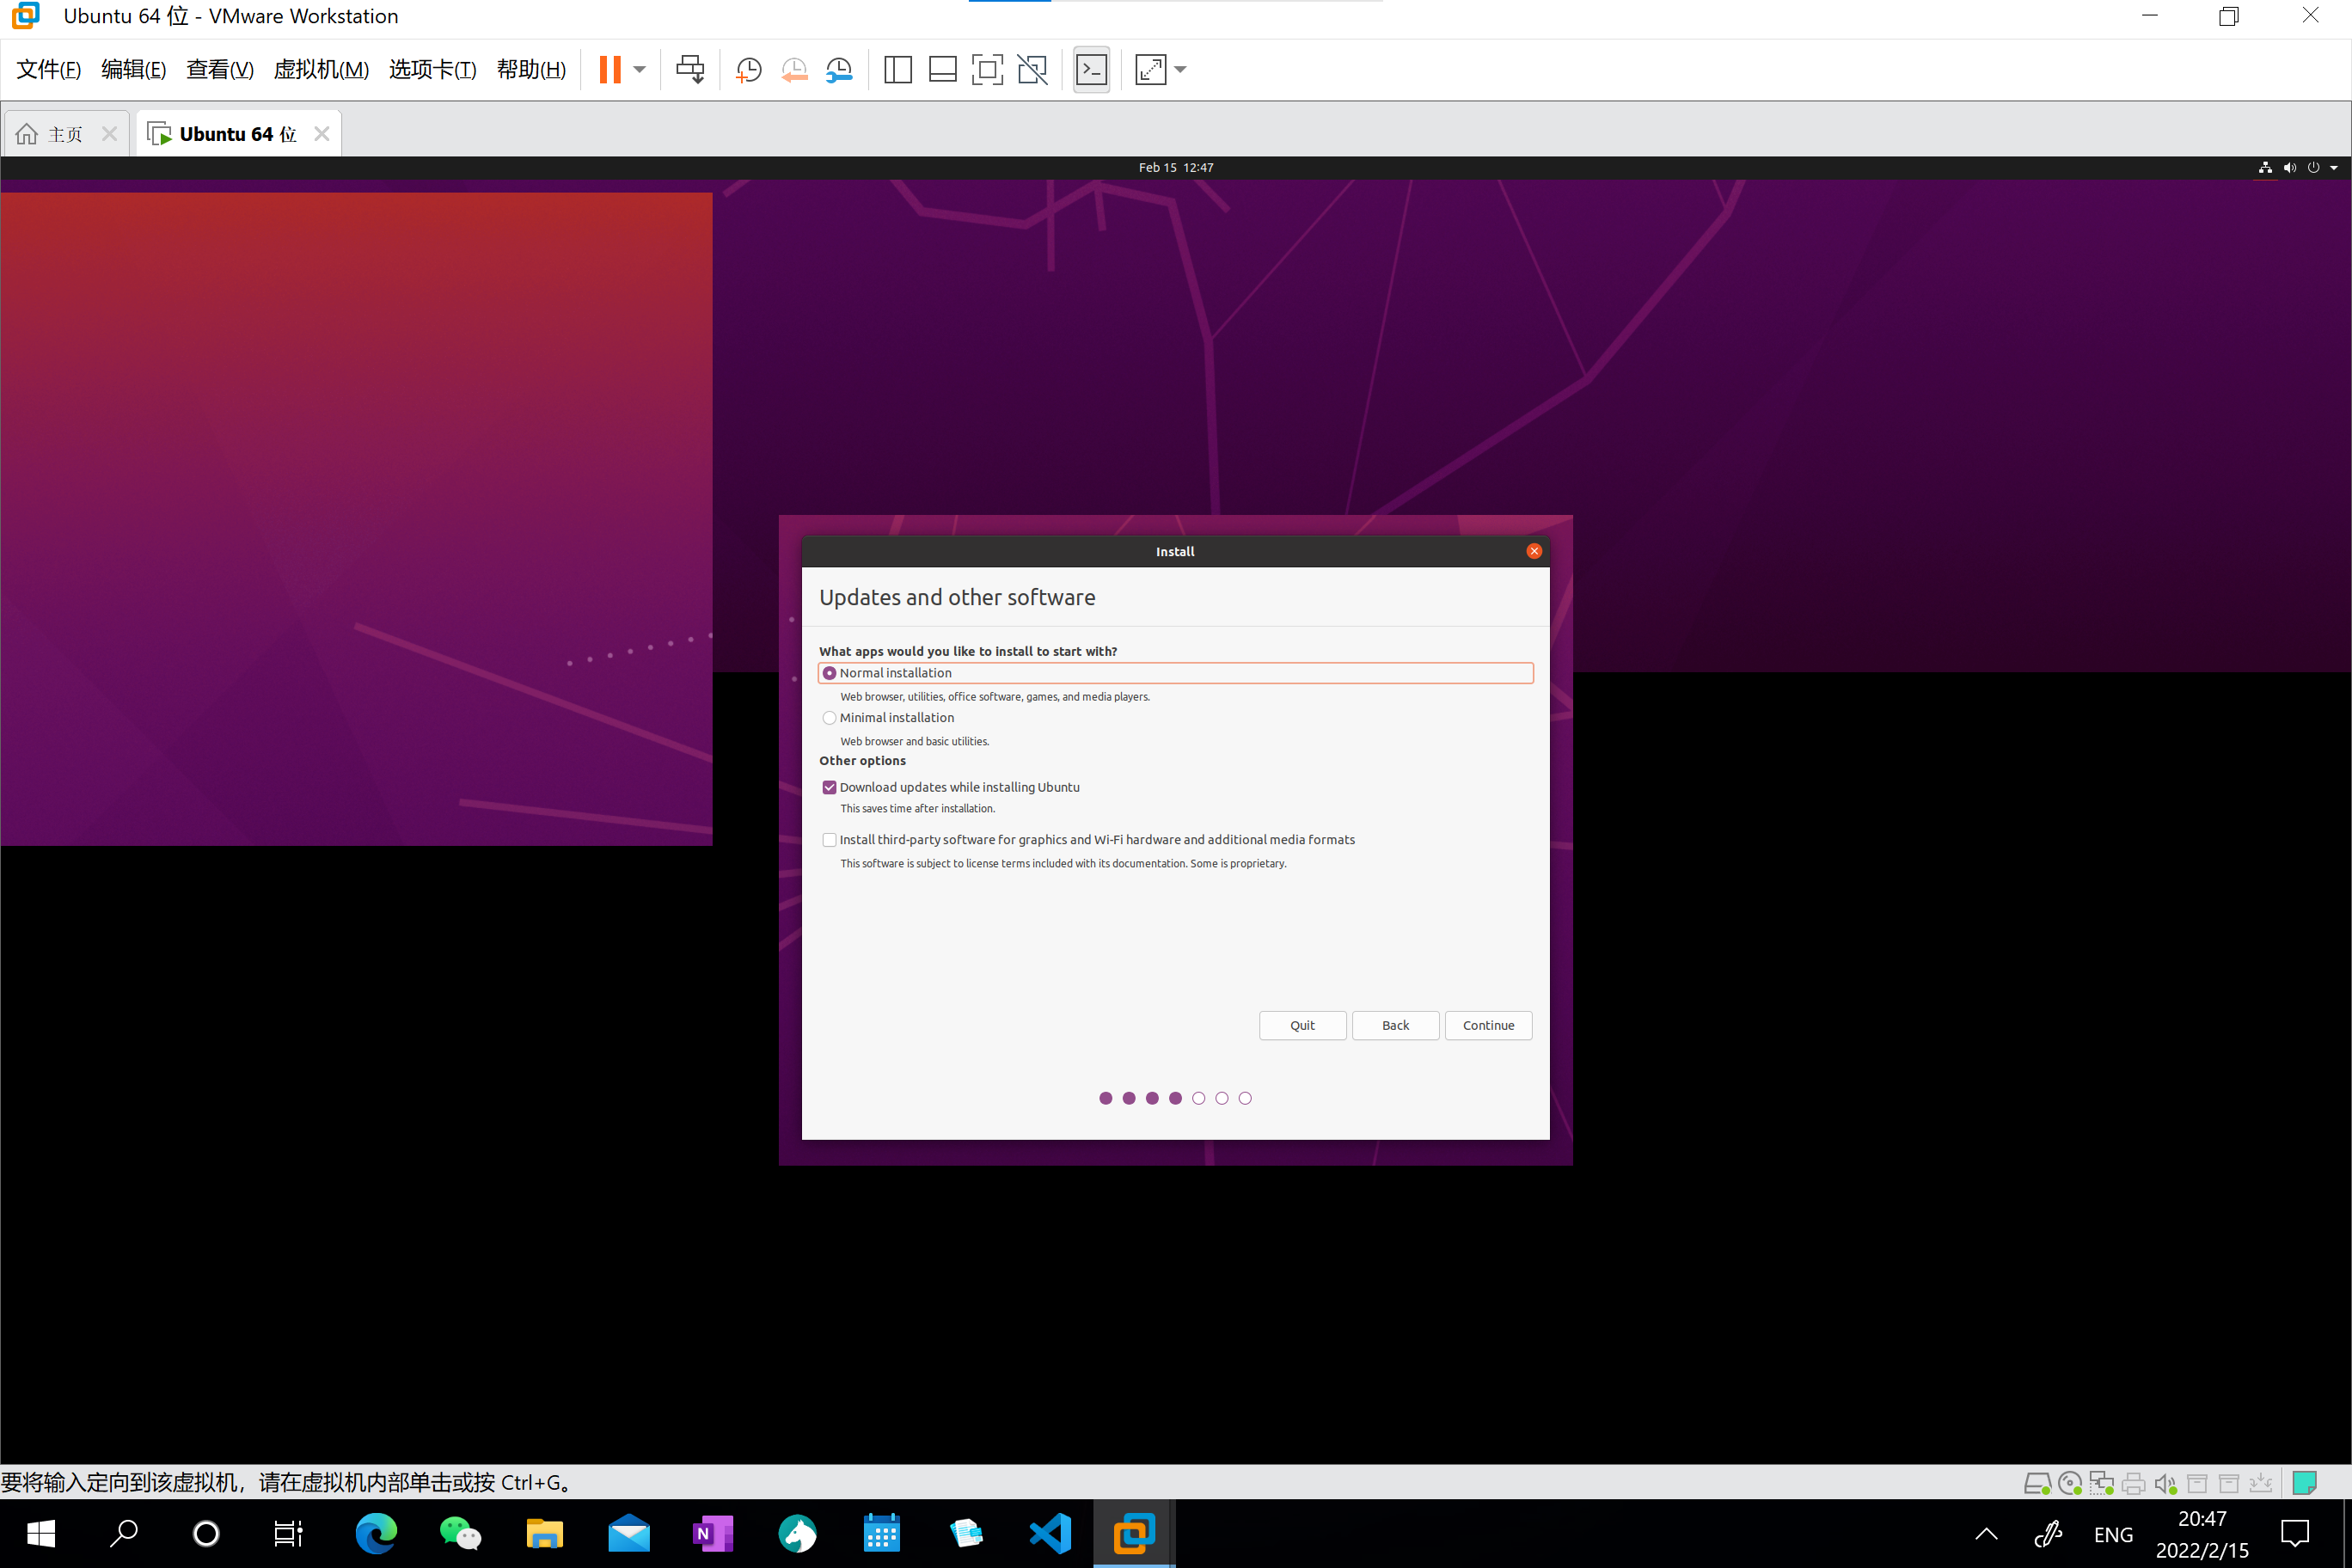
\includegraphics[width=0.8\textwidth]{assets/l2.png}
    \end{figure}   
    \begin{figure}[H]
        \centering
        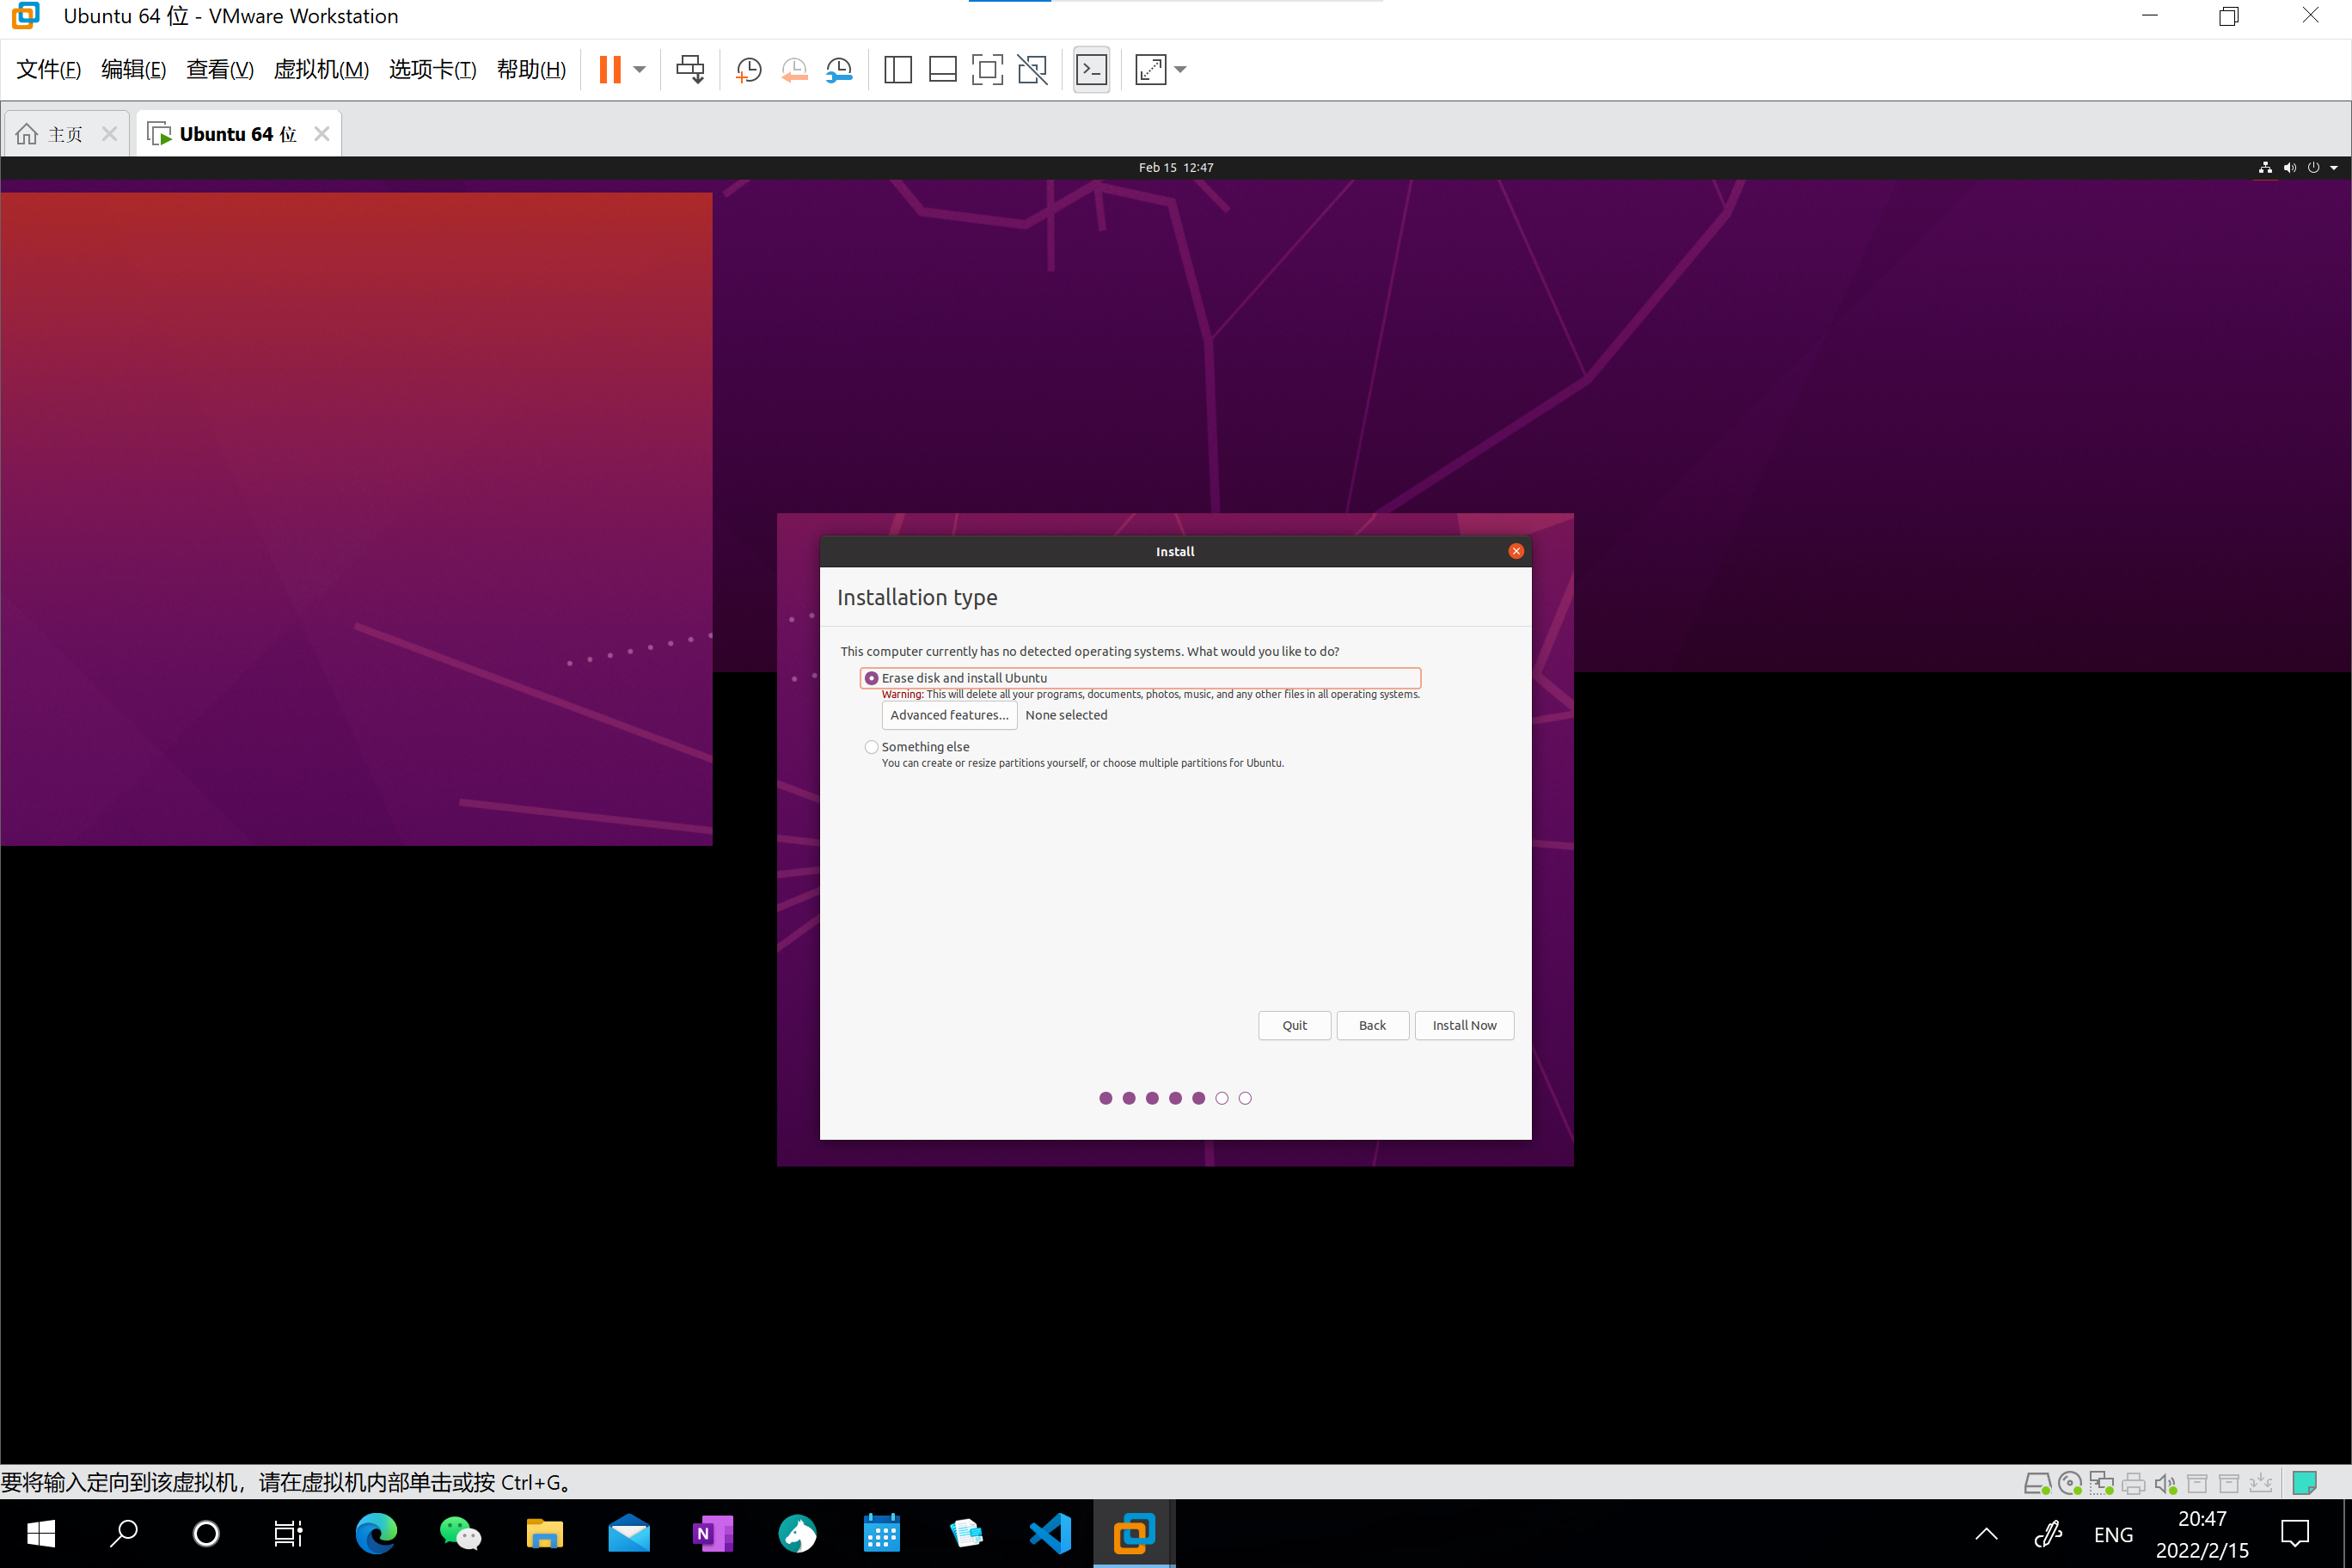
\includegraphics[width=0.8\textwidth]{assets/l3.png}
    \end{figure}
    \begin{figure}[H]
        \centering
        \includegraphics[width=0.8\textwidth]{assets/l4.png}
    \end{figure}
    \begin{figure}[H]
        \centering
        \includegraphics[width=0.8\textwidth]{assets/l5.png}
    \end{figure}

    \section{运行命令行}
    安装步骤完成后,重启虚拟机,即可完成安装。
    \par 打开命令行,执行命令 date 以及 uname -a ,执行结果如下:(在之前安装的其他版本ubuntu上运行)
    \begin{figure}[H]
        \centering
        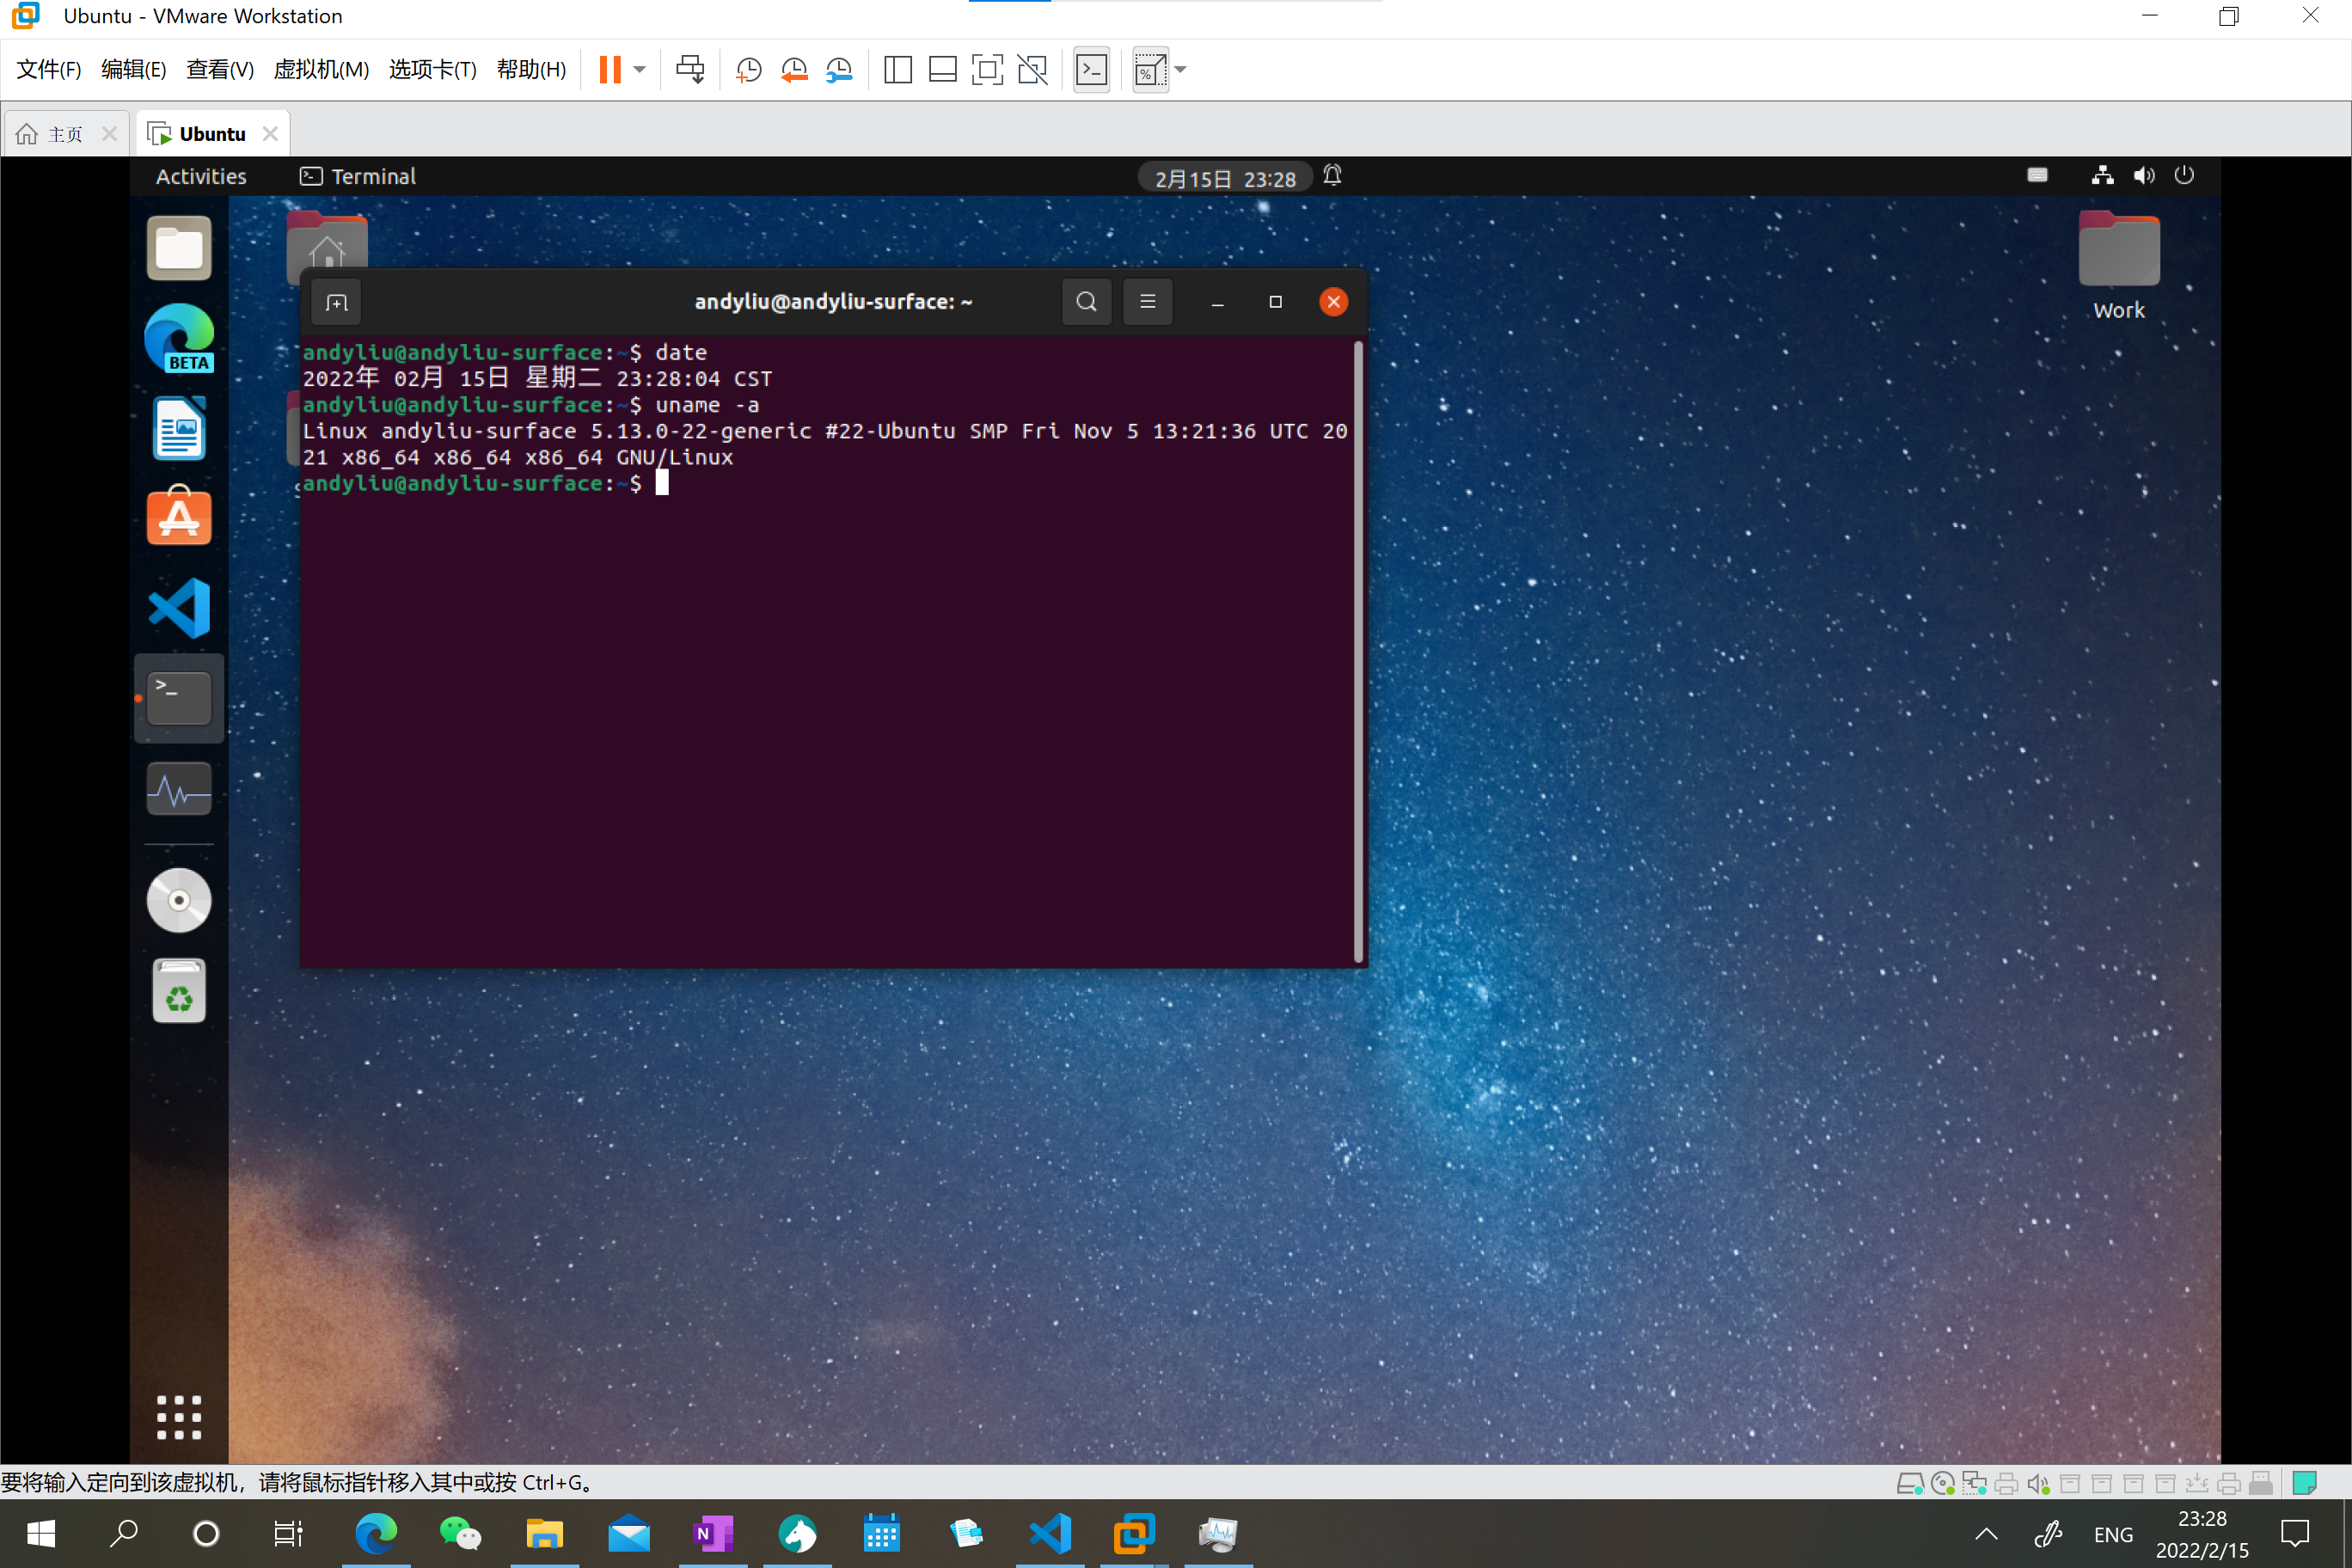
\includegraphics[width=0.8\textwidth]{assets/l6.png}
    \end{figure}

\end{document}